% !TeX spellcheck = de_DE
\documentclass[IWBstudentthesis%     style
              ,optCharter%           font
              %,optCMYK%             color model
              ,optBibtex% 	         bibliography tool
              ,optBibstyleNumeric%lbam (ieee) citation style
              ,optEnglish% 		 language
              %,optTikzExternalize%  compiles faster for large tikz images
              ]{IWBlatex}%
%
% Set paths
\graphicspath{{figures/}}%
\addbibresource{source/literature.bib}%
\makenoidxglossaries%
%A--------------------------------------------------------
\newacronym{am}{AM}{Additive Manufacturing}%
%C--------------------------------------------------------
\newacronym{cad}{CAD}{Computer Aided Design}%
%I--------------------------------------------------------
\newacronym{mas}{MAS}{Multi-Agent System}%

\newacronym{dai}{DAI}{Distributed Artificial Intelligence}%

\newacronym{ra}{RA}{Resource Agent}%
\newacronym{ras}{RAs}{Resource Agents}%
\newacronym{ca}{CA}{Communication Agent}%
\newacronym{ams}{AMS}{Agent Management System}%
\newacronym{cda}{CDA}{Coordinator Agent}%
\newacronym{mfs}{MFS}{Material Flow System}%
\newacronym{plm}{PLM}{Product Lifecycle Management}%
\newacronym{dta}{DTA}{Digital Twin Agent}%
\newacronym{dt}{DT}{Digital Twin}%
\newacronym{dsl}{DSL}{Domain Specific Language}%
\newacronym{gpl}{GPL}{General Purpose Language}%
\newacronym{cps}{CPS}{Cyber Physical System}%
\newacronym{af}{AF}{Adaptable Factory}%
\newacronym{db}{DB}{Database}%
\newacronym{fdd}{FDD}{Fault Detection And Diagnostics}%
\newacronym{tcp}{TCP}{Transmission Control Protocol}%
\newacronym{udp}{UDP}{User Diagram Protocol}%
\newacronym{mqtt}{MQTT}{Message Queuing Telemetry Transport}%
\newacronym{http}{HTTP}{Hypertext Transfer Protocol}%
\newacronym{ms}{MS}{Microsoft}%
\newacronym{utc}{UTC}{Coodinated Universal Time}%
\newacronym{ntp}{NTP}{Network Time Protocol}%
\newacronym{rcp}{RCP}{Robot Control Program}%
\newacronym{osi}{OSI}{Open Systems Interconnection}%
\newacronym{kql}{KQL}{Kusto Query Language}%
\newacronym{tcp/ip}{TCP/IP}{Transmission Control Protocol/Internet Protocol}%
\newacronym{iot}{IoT}{Internet Of Things}%
\newacronym{rci}{RCI}{Robot Control Interface}%
\newacronym{cpu}{CPU}{Central Processing Unit}%
\newacronym{crud}{CRUD}{Create, read, update and delete}%
\newacronym{rtt}{RTT}{Round-Trip Time}%
\newacronym{owd}{OWD}{One-Way Delay}%
\newacronym{uml}{UML}{Unified Modeling Language}%
\newacronym{dps}{DPS}{Distributed Problem Solving}%
\newacronym{aas}{AAS}{Asset Administration Shell}%
\newacronym{ftt}{FTT}{Funk Transfer Tester}%
\newacronym{rviz}{RViz}{ROS visualization}%
\newacronym{nic}{NIC}{Network Interface Card}%
\newacronym{mac}{MAC}{Medium Access Control}%

%----------------------------
\newacronym{ir}{IR}{infrared}%
\newacronym{iwb}{\textit{iwb}}{Institut für Werkzeugmaschinen und Betriebswissenschaften}%
%L--------------------------------------------------------
\newacronym{lbam}{LBAM}{Professorship Laser-based Additive Manufacturing}%
%M--------------------------------------------------------
\newacronym{ml}{ML}{Machine Learning}%
%P--------------------------------------------------------

\newacronym{pbf}{PBF}{Powder Bed Fusion}%
\newacronym{pbflb}{PBF-LB}{Laser-based Powder Bed Fusion}%
\newacronym{pbflbp}{PBF-LB/P}{Laser-based Powder Bed Fusion of Polymers}%
%R--------------------------------------------------------
\newacronym{ros}{ROS}{Robot Operating System}%
\newacronym[\glslongpluralkey={Arbeitspakete}]{ap}{AP}{Arbeitspaket}%
%s--------------------------------------------------------
\newacronym{sls}{SLS}{Selective Laser Sintering}%
%s--------------------------------------------------------
%
\newglossaryentry{latex}%
{%
	name=Latex,%
	description={Generische Mark-up-Sprache zum Erstellen wissenschaftlicher Texte. Sie ist in jeder Hinsicht Word überlegen, welches einem visuellen Mark-Up entspricht. Das X von \LaTeX\ wird als ç (Stimmloser palataler Frikativ) ausgesprochen, vergleiche deutsche Aussprache von \textit{ch}.}%
}%
\newglossaryentry{tutorial}%
{%
	name=Tutorial,%
	description={Kurze Gebrauchsanleitung welche ein Thema, einen gewissen Vorgang oder eine Funktion erklärt. Hat nicht den Anspruch auf Vollständigkeit.}%
}%
\newglossaryentry{tikz}%
{%
	name=Ti\textit{k}Z,%
	description={Frontend-Paket, das auf PGF-Plot aufbaut und zum Erstellen von Graphiken dient.}%
}%%
% Custom macros
% Einheitliche Schreibweise
% ---------------------------------------
\newcommand{\zb}{z.\,B.\xspace}%
\renewcommand{\dh}{d.\,h.\xspace}%
\newcommand{\uu}{u.\,U.\xspace}%
\newcommand{\ua}{u.\,a.\xspace}%
\newcommand{\idr}{i.\,d.\,R.\xspace}%
\newcommand{\vgl}{vgl.\xspace}%
\newcommand{\sa}{s.\,a.\xspace}%
\newcommand{\bzw}{bzw.\xspace}%
\newcommand{\evtl}{evtl.\xspace}%
\newcommand*{\eg}{e.\,g.\xspace}%
\newcommand*{\ie}{i.\,e.\xspace}%
% Leichtere Zitate
% ---------------------------------------
% \cite{} gut für Shorthand (Normen) im Text --> alternative zu \textcite
\newcommand{\autor}[2]{\textcite[#1]{#2}}%
\newcommand{\zitat}[2]{\parencite[#1]{#2}}%
\newcommand{\zitatpre}[3]{\parencite[#1][#2]{#3}}%
\newcommand{\zitate}[4]{\parencites[#1]{#2}[#3]{#4}}%
\newcommand{\zitatee}[6]{\parencites[#1]{#2}[#3]{#4}[#5]{#6}}%
\newcommand{\zitateee}[8]{\parencites[#1]{#2}[#3]{#4}[#5]{#6}[#7]{#8}}%
% ---------------------------------------
\newcommand{\insertref}{\todo[color=green!40]{Missing ref}}%
% Leichtere Bilder
% ---------------------------------------
\newcommand{\bild}[4]{%
	\begin{figure}[#1]
		\centering
		\includegraphics
		[
		width=#2\textwidth,
		]
		{figures/#3}
		
		\caption{#4}
		\label{fig:#3}
	\end{figure}
}
%
%
\newcommand{\bildsvg}[4]{
	\begin{figure}[#1]
		\centering%
		\def\svgwidth{#2\columnwidth}%
		\input{figures/#3}%
		%
		\caption{#4}%
		\label{fig:#3}%
	\end{figure}	
}
%
\newcommand{\bildtikz}[4]{
	\begin{figure}[#1]
		\centering
		\scalebox{#2}{\input{figures/#3}}
		\caption{#4}
		\label{fig:#3}
	\end{figure}
}
%
\newcommand{\bildtikzvar}[5]{
	\begin{figure}[#1]
		\centering
		\scalebox{#2}{\input{figures/#3}}
		\caption{\parbox[t]{#4\textwidth}{#5}}
		\label{fig:#3}
	\end{figure}
}
%
\newcommand{\bildtrim}[5]{% Mit definiertem Beschnitt
	\begin{figure}[#1]
		\centering
		\includegraphics
		[
		width=#2\textwidth,
		%keepaspectratio=true,
		trim=#3,		% l u r o
		clip,
		]
		{figures/#4}
		
		\caption[]{#5}
		\label{fig:#4}
	\end{figure}
}
%
\newcommand{\bildvar}[5]{% Mit definierter Breite / Zeilenumbruch der Caption
	\begin{figure}[#1]
		\centering
		\includegraphics
		[
		width=#2\textwidth,
		]
		{figures/#3}
		
		\caption[]{\parbox[t]{#4\textwidth}{#5}}
		\label{fig:#3}
	\end{figure}
}
%
\newcommand{\bildbox}[4]{% Bild mit Rahmen
	\begin{figure}[#1]
		\centering
		\fbox{%
			\includegraphics
			[
			width=#2\textwidth,
			]
			{figures/#3}
		}
		\caption[]{#4}
		\label{fig:#3}
	\end{figure}
}
%
\newcommand{\bildboxtrim}[5]{%
	\begin{figure}[#1]
		\centering
		\fbox{%
			\includegraphics
			[
			width=#2\textwidth,
			%keepaspectratio=true,
			trim=#3,		% l u r o
			clip,
			]
			{figures/#4}
		}
		\caption[]{#5}
		\label{fig:#4}
	\end{figure}
}
%
\newcommand{\bildboxvar}[5]{%
	\begin{figure}[#1]
		\centering
		\fbox{%
			\includegraphics
			[
			width=#2\textwidth,
			]
			{figures/#3}
		}
		\caption[]{\parbox[t]{#4\textwidth}{#5}}
		\label{fig:#3}
	\end{figure}
}
%
\newcommand{\bildsvgvar}[5]{
	\begin{figure}[#1]
		\centering
		\def\svgwidth{#2\columnwidth} 
		\subimport*{figures/}{#3}
		\caption{\parbox[t]{#4\textwidth}{#5}}
		\label{fig:#3}
	\end{figure}	
}
%
\newcommand{\bildpdf}[3]{%
	\begin{figure}[H]
		\centering
		\includegraphics
		[
		width=#1\textwidth,
		page={#2},
		]
		{#3}
		%\caption[]{#4}
		\label{fig:#3}
	\end{figure}
}
% ---------------------------------------%
%
% Extra packages for LBAM formatting-------------------------------------------
% continous figure and table counter (arabic numbers Fig 1., Fig 2. etc. not Fig. 1.1, Fig 1.1)
\usepackage{chngcntr}%
\counterwithout{figure}{chapter}%
\counterwithout{table}{chapter}%
%--------------------------------------
%packages my paper:

\usepackage{array}
\usepackage{makecell}
\usepackage{graphicx}


\usepackage{rotating}
\usepackage{caption}

\usepackage{algorithm}
% \usepackage[fleqn]{amsmath}
%\usepackage{algorithmic}
%\usepackage{algpseudocode}


\usepackage[noend]{algpseudocode} % This provides the algorithmic environment and is part of algorithmicx package.


\begin{document}%
% Titlepage
% ---------
\frontmatter%
% Info: replace Prof Reinhart by Prof. Zäh:\IWBnamesProfZaeh \newline \IWBlangChairMWIWBLWF
% Info: separate multiple supervisors by \newline
\IWBstudentthesisTitlePageCustomSemesterThesis{Modellierung und Analyse von Kommunikations-\\verzögerungen in Multi-Agent-Systemen mit zwei Anwendungsfällen}{Modeling and Analyzing Communication \\Delays in Multi-Agent System with Two \\Industry Use Cases}{Xuezhou Hou \newline Willi-Graf-Straße 5 \newline 80805 München}{\IWBnamesProfVogelHeuser \newline M.Sc. Jingyun Zhao \newline M. Sc. Fandi Bi \newline \IWBlangChairMWAIS}{\IWButilsDate{15}{11}{2023}}%
%
%\IWBstudentthesisTitlePageCustomBachelorsThesis{German Title}{English Title}{Martin Mustermann \newline Musterweg 20 \newline 80999 München}{\IWBnamesProfReinhart \newline \IWBlangChairMWIWBLBM}{\IWButilsDate{1}{1}{2018}}%
%
%\IWBstudentthesisTitlePageCustomSemesterThesis{German Title}{English Title}{Martin Mustermann \newline Musterweg 20 \newline 80999 München}{\IWBnamesProfReinhart \newline \IWBlangChairMWIWBLBM}{\IWButilsDate{1}{1}{2018}}%
%
%\IWBstudentthesisTitlePageCDIDP{German Title}{English Title}{Martin Mustermann \newline Musterweg 20 \newline 80999 München}{\IWBnamesProfReinhart \newline \IWBlangChairMWIWBLBM}{\IWButilsDate{1}{1}{2018}}%
%
% Task formulation
% ----------------
% Deckblatt
\chapter*{Scope of Work}

%\markright{Aufgabenstellung} 	% Kolumnentitel manuell auf "Aufgabenstellung"

\textbf{Title of the Master's Thesis:}\\
\Large{Manually Change you Thesis Title here}\\
%\newline
%\normalsize{\textbf{(English Title of the Bachelor's/Master's Thesis/Semester Thesis/In\-ter\-dis\-ci\-pli\-na\-ry Project:)}}\\
%\Large{Development...}
\normalsize

\begin{tabbing}
	\hspace{7em} 		\= \hspace{13em}			\= \hspace{7em} 		\= \kill
	\textbf{Author:}  \> B.Sc. Max Mustermann 	\> \textbf{Supervisor:} 	\>  M.Sc. Mein Betreuer \\
	\textbf{Issuance:} 	\> 01.07.2021 	\> \textbf{Submission:} 	\> 31.12.2021
\end{tabbing}

\vspace{5mm}
\textbf{Setting:}\\
\blindtext%

\vspace{5mm}
\textbf{Objective:}\\
\blindtext

\vspace{5mm}
\textbf{Methodology:} \\
The content of the present thesis can be subdivided into the following tasks
\begin{itemize}
	\item Method 1
	\item Method 2
	\item Method 3
	\item etc.
\end{itemize}
\vspace{1.0cm}

\chapter*{Declaration}
I hereby confirm that this master's/ bachelor's/ semester thesis was written independently by myself without the use of any sources beyond those cited, and all passages and ideas taken from other sources are cited accordingly.%
%
\vspace{5cm}\\
\begin{tabular}{p{0.5\linewidth}p{0.5\linewidth} }
	.....................................................		& .....................................................\\
	Location, Date  	& Signature
\end{tabular}
%
\vspace{2cm}\\
%
With the supervision of Prof. Dr.-Ing. Birgit Vogel-Heuser by M.Sc. Jingyun Zhao
and M.Sc. Fandi Bi intellectual property of the \gls{ais} flows into this work. A publication of the work or a passing on to third parties requires the permission of the head of the professorship. I agree to the archiving of the printed thesis in the  \gls{ais} library (which is only accessible to \gls{ais} staff) and in \gls{ais}'s digital thesis database as a PDF document.%
%
\vfill
%
\begin{tabular}{p{0.5\linewidth}p{0.5\linewidth} }
	.....................................................		& .....................................................\\
    Location, Date  	& Signature
\end{tabular}
%
%
% Abstract
% --------
% In total max. 1 Page!
\IWBstudentthesisAbstract{%
	%
	% Abstract English:
	In the context of Industry 4.0, \gls{mas} plays a pivotal role in the 
	decentralization of \gls{cps}, and \gls{dt} contributes to the digitalization 
	of physical entities for \gls{plm}. This study aims to provide a solution for 
	\gls{mas} design in a more structured way, including the modularization of the 
	agent's capabilities based on Wannagat's architecture and the modularization of 
	network-based communication delays inherited from the soft and hard real-time 
	requirement of the automation and robot-like production system. The system 
	design consists of two parts: part 1, the local \gls{mas} to enable agent's 
	scheduling and coordination, decision-making and planning, and most 
	importantly, real-time communication under a 5G wireless network, and part 2, 
	the design of a \gls{dta} to transmit robot's process data to the global 
	\gls{dt} and back to the local device. Based on the system design, tests 
	have been conducted for both parts to analyze their timing properties under 
	different conditions, including worst-case scenarios. Additionally, two use 
	cases are applied to the local \gls{mas} system design, with the BMW use case 
	tested for its timing behaviors. Finally, a modular system design consideration 
	based on \gls{dsl} is provided, presented as a set of interconnected graphical notations 
	for the \gls{mas}. %
}{%
	%
	% Zusammenfassung Deutsch:
	Im Kontext von Industrie 4.0 spielt \gls{mas} eine zentrale Rolle bei der 
	Dezentralisierung von \gls{cps} und \gls{dt} trägt zur Digitalisierung 
	physischer Einheiten für \gls{plm} bei. Ziel dieser Studie ist es, eine 
	strukturiertere Lösung für das \gls{mas}-Design bereitzustellen, einschließlich 
	der Modularisierung der Fähigkeiten des Agenten auf der Grundlage der 
	Wannagat-Architektur und der Modularisierung netzwerkbasierter 
	Kommunikationsverzögerungen, die aus den weichen und harten 
	Echtzeitanforderungen übernommen wurden der Automatisierung und des 
	roboterähnlichen Produktionssystems. Das Systemdesign besteht aus zwei 
	Teilen: Teil 1, dem lokalen \gls{mas}, um die Scheduling und Koordination, 
	Entscheidungsfindung und Planung des Agenten und vor allem die 
	Echtzeitkommunikation unter einem 5G-Wireless-Netzwerk zu ermöglichen, 
	und Teil 2, der Entwurf eines \gls{dta} zur Übertragung der Prozessdaten 
	des Roboters an das globale \gls{dt} und zurück an das lokale Gerät. 
	Basierend auf dem Systemdesign wurden Tests für beide Teile durchgeführt, 
	um ihre Timing-Eigenschaften unter verschiedenen Bedingungen, einschließlich 
	Worst-Case-Szenarien, zu analysieren. Darüber hinaus werden zwei 
	Anwendungsfälle auf das lokale \gls{mas}-Systemdesign angewendet, 
	wobei der BMW-Anwendungsfall auf sein Zeitverhalten getestet wird. 
	Abschließend wird eine Überlegung zum modularen Systemdesign basierend 
	auf \gls{dsl} bereitgestellt, präsentiert als eine Reihe miteinander verbundener 
	grafischer Notationen für \gls{mas}.%
}%
%
%%
%
% Content
% -------
\IWBstudentthesisPrintTableOfContents%
%
% List of Abbreviations --> for LBAM moved to end document
% ---------------------
%\printnoidxglossary[type=acronym,sort=standard,title={\IWBlangAcronyms}]
%
% Mainmatter
% ----------
\mainmatter%
% !TeX spellcheck = de_DE
\chapter{LaTeX-Tutorial}%
Dieses \gls{tutorial} liefert eine Kurzeinführung in die Verwendung von \gls{latex}.%
%
\section{Titelseite}%
Die Titelseite wird in {./main.tex} definiert. Der Studienarbeitstyp wird durch Ein- und Auskommentieren der Befehle%
\begin{itemize}%
	\item \verb|\IWBstudentthesisTitlePageCustomMastersThesis|,%
	\item \verb|\IWBstudentthesisTitlePageCustomBachelorsThesis| und%
	\item \verb|\IWBstudentthesisTitlePageCustomSemesterThesis|%
\end{itemize}%
ausgewählt und die Seite entsprechend der Argumente gesetzt. Die Professoren und Lehrstuhle können mittels der Makros%
\begin{itemize}%
	\item \verb|\IWBnamesProfReinhart \newline \IWBlangChairMWIWBLBM| oder%
	\item \verb|\IWBnamesProfZaeh \newline \IWBlangChairMWIWBLWF|%
\end{itemize}%
ausgewählt werden.%
%
\section{Zitation}%
%
Zum Zitieren stehen die Standartbefehle \verb|\textcite| und \verb|\parencite| zur Verfügung. Soll der Autorename im Satz verwendet werden, eignet sich ersteres, z.B. \textcite[2-3]{Bayerlein2018} bezieht sich auf \textcite{Bayerlein2016469}. Soll das Zitat in Klammern nach die Aussage gestellt werden empfiehlt sich zweiteres \parencite{Zaeh2018385}. Sammelzitationen am Satzende schreiben sich wie folgt \parencite{Kleinwort2018658,Kleinwort20189,Kleinwort2018631}. Die Zitation von Online-Quellen kann schwierig sein, da nicht immer der Autor und das Erscheinungsjahr verfügbar sind. Vergleicht man \textcite{Heuss2018} und \textcite{iwb-Startseite}, stellt man fest, dass bei zweiteren der Seitentitel statt des bekannten Schemas eingesetzt wird.\par%
%
Normen werden als \textcite{ISO.10218-2} dargestellt. Im Bibtex-Export des verwendeten Literaturverwaltungsprogramm sind bestimmte Einstellungen vorzunehmen. Dokumententyp ist \enquote{@book} mit folgenden Einträgen:
\begin{itemize}
	\item Normtyp und Nummer als \enquote{title}
	\item Langtitel als \enquote{subtitle}
	\item Verlag als \enquote{publisher}
	\item Jahr als \enquote{date}
	\item \enquote{author} darf nicht belegt werden!
\end{itemize}
%
\section{Abkürzungen}
In {./source/abbreviations.tex} können Abkürzungen definiert werden. Es gibt Besonderheiten zu Ausdrücken, deren Pluralendung nicht auf s endet. Hier müssen ggf. Kurz- und Langformen des Ausdrucks auch für den Plural definiert werden.\par%
\begin{itemize}
	\item \verb|\gls{ros}|: schreibt beim ersten Auftreten im Dokument ausführlich \gls{ros}, ab dem zweiten Auftreten wird abgekürzt \gls{ros}% 
	\item \verb|\glspl{ap}| verwendet den Plural in Langform \glspl{ap} und danach in Kurzform \glspl{ap}%
\end{itemize}%
%
\section{Glossar}
In {./source/glossary.tex} können Begriffe erklärt, abgegrenzt oder definiert werden. Begriffe erhalten einen Namen und eine Beschreibung als Glossareintrag sowie ein Lable zum Referenzieren im Text. Ein Glossar ist Optional.\par%
\begin{itemize}%
	\item \verb|\gls{latex}|: Schreibt den Namen aus dem Glossarverzeichnis mit Verweis auf den Glossareintrag \gls{latex}%
\end{itemize}%
%
\section{Abbildungen}
Graphiken und Bilder können in beliebigen Dateiformaten eingebunden werden, vergleiche \cref{fig:MyImage}. Vektorgraphiken sind im Allgemeinen Pixelgraphiken in Schärfe und Speicherbedarf überlegen.\par%
%
\begin{figure}[htb]%
    \centering%
    %
    % Including .png
    
\includegraphics[width=40mm]{figures_tutor/ImagePNG.png}%
    %
    \hspace*{5mm}%
    %
    % Including .pdf
    
\includegraphics[width=40mm]{figures_tutor/ImagePDF.pdf}\par%
    %
    % Including .tikz
    \begingroup%
        %\AMtikzExternalizeSkipNext%
        \resizebox{40mm}{!}{\begin{tikzpicture}[inner sep=0pt, outer sep=0pt]%
    \fill [draw=TUMBlue,line width=5mm,fill=none] (0mm,0mm) rectangle (95mm,95mm);%
    \node at (50mm,50mm) {\fontsize{60}{60}\selectfont TIKZ};%
\end{tikzpicture}%
}%
    \endgroup%
    %
    \hspace*{5mm}%
    %
    % Including .pdf_tex
    \begingroup%
        \def\svgwidth{40mm}%
        \fontsize{25}{25}\selectfont%
        \input{figures_tutor/ImagePDFTEX.pdf_tex}%
    \endgroup%
    %
    \caption{Beschreibung des Bilds. Außerdem machen wir nun die Bildunterschrift unnötig lang um die Formatierung zu testen. \label{fig:MyImage}}%
\end{figure}%
%
\begin{figure}[htb]%
    \centering%
    \small%
\pgfplotstableread{figures_tutor/datatable2d.dat}{\datatableTwoDim}%
\begin{tikzpicture}[scale=1]%
    \begin{axis}[width = 9cm, height = 6cm, scale only axis=true%
                 ,xmin = 0%
                 ,xmax = 10%
                 ,xlabel = {$t$ in s}%
                 ,xtick distance = 1%
                 ,ymin = -1.2%
                 ,ymax = 1.2%
                 ,ylabel = {y-Label}%
                 ,ytick distance = 0.5%
                 ,grid = both%
                 ,grid style = {line width = .1pt, draw = TUMBlack!10}%
                 ,legend style = {at = {(0.1cm,0.1cm)}, anchor = south west,font=\small}%
                 ,\IWBlangGerEng{/pgf/number format/use comma}{}%
                 ]%
        \addplot [TUMBlue,very thick] table [x={X}, y={Y1}] {\datatableTwoDim};%
        \addplot [TUMBlue3,very thick,dashed] table [x={X}, y={Y2}] {\datatableTwoDim};%
        \addplot [TUMBlack,very thick,dotted] table [x={X}, y={Y3}] {\datatableTwoDim};%
        \legend{$\sin(t)$,$\cos(t)$,$0.5$};%
    \end{axis}%
\end{tikzpicture}%
%
%
%
    \caption{Beschreibung des Plots. Außerdem machen wir nun die Bildunterschrift unnötig lang um die Formatierung zu testen. \label{fig:PlotTwoDim}}%
\end{figure}%
%
Für Nutzer mit perfektionistischen Anspruch empfiehlt sich die Nutzung von \gls{tikz}. Vorteil ist, dass die Erzeugung von Daten und die Darstellung komplett getrennt werden. Die Darstellung erfolgt einheitlich gemäß eines generischen Mark-Ups, vergleiche \cref{fig:PlotTwoDim,fig:PlotThreeDim}.\par%
%
\vspace{12pt}%
\begin{figure}[htb]%
    \centering%
    \small%
\pgfplotsset{colormap={mycolormap}{rgb255=(255,255,0) rgb255=(255,0,0)}}%    
\begin{tikzpicture}%
    \begin{axis}[width = 10cm, height = 8cm%
                ,xmin = -1%
                ,xmax = 1%
                ,xlabel = {$x$ in m}%
                ,xtick distance = 0.5%
                ,ymin = -1%
                ,ymax = 1%
                ,ylabel = {$y$ in m}%
                ,ytick distance = 0.5%
                ,zmin = 0%
                ,zmax = 1%
                ,zlabel = {$z$ in m}%
                ,ztick distance = 0.2%
                ,grid = both%
                ,grid style = {line width = .1pt, draw = TUMBlack!10}%
                ,colorbar%
                ,view={60}{30}%
                ,\IWBlangGerEng{/pgf/number format/use comma}{}%
                ]%
        \addplot3 [surf,z buffer=sort] table[x={X}, y={Y}, z={Z}] {figures_tutor/datatable3d.dat};%
    \end{axis}%
\end{tikzpicture}%
%
%
%
    \caption{Beschreibung des Plots. Außerdem machen wir nun die Bildunterschrift unnötig lang um die Formatierung zu testen. \label{fig:PlotThreeDim}}%
\end{figure}%
%
%
%
% !TeX spellcheck = en_US
\glsresetall%
\chapter{Introduction}%
This article is written to raise readers' interest in the necessity of 
analyzing communication delays between each participant in a general 
\gls{mas} based on two industry use cases in a more modular way. 
Before getting deep into the actual work of the research, 
a brief motivation followed by the research questions will be
provided to guide this study.

\section{Motivation}\label{chap: Motivation}
The requirements of modern industrial production have become more and 
more crucial due to the increased complexity of interconnections of 
various robots and automation systems during manufacturing. Different 
from the production mode of a traditional factory, the concept of a 
smart factory of Industry 4.0 has been developed to overcome the 
remaining issues, such as the high centralization of a traditional 
control system, low scalability of production systems, and processes, 
limited adaptability of new conditions and requirements with changing 
environments, hardness of real-time decision making, insufficient resource 
allocation and many more. Under this prerequisite, a \gls{mas} plays a crucial 
part in closing the gaps. 


The precursor to modern \gls{mas} is \gls{dai}, which focuses on distributing a 
single complex AI task to multiple machines and processors\cite{noauthor_jacques_nodate}, 
which is nowadays classified into parallel AI, \gls{dps}, and \gls{mas}\cite{dorri_multi-agent_2018}. 
With the focus on \gls{mas} in this article, it can be described as a combination of 
autonomous agents and their environments. However, the complete decomposition of 
the complex real-world system can be challenging, which leaves space for self-learning 
and decision-making in a primitive level of agent autonomy\cite{reis_applications_2004}. 
The concept of resource distribution/decentralization is inherited by \gls{mas} to 
handle more distributed and interconnected computing tasks. It results in a more 
intelligent and autonomous agent-based operation system in which each agent can make 
decisions independently to achieve its own goal. At the same time, they still tend 
to collaborate, negotiate, and coordinate with other agents frequently in order to 
improve the efficiency and quality of production workflow meanwhile reducing 
cost \cite{vogel-heuser_multi-agent_2020}. In a \gls{mas}, agents have the ability 
to interact with one another, perceive their surroundings, and adapt to rapid changes 
in the environment. This collective capability enables them to solve complex problems 
that a single agent would not be able to handle alone. 

% check from here with grammarly
Effective communication between agents is crucial for the successful functioning of a 
system\cite{georgeff_communication_1988}. According to the discussion of agent 
communication\cite{vogel-heuser_multi-agent_2020}, in addition to the horizontal 
communication between agents, the vertical communication between assets 
and their mapped \gls{aas} can also be realized by agents to extend the domain 
of \gls{mas}. \gls{aas} is a standard 
that serves as the foundation of the \gls{dt} implementation\cite{redeker_towards_2021}. 
To differentiate, \gls{aas} provides a data structure for \gls{dt}, while Digital 
Twin uses the data for real-time data representation, simulation, and analysis. 
The concept of \gls{dt} was first introduced by Michael 
Grieves \cite{flumerfelt_complex_2019}, who also introduce the 
famous \gls{plm} model \cite{greengard_digital_nodate}to 
explain the role of a in the product lifecycle. Data from engineering, 
design and manufacture should be digitalized to represent physical 
assets. Some common understandings of engineering data could be 
for example simulation for performance testing. Or may be design data 
that builds a visual representation of CAD data of plants and robots, 
and manufacture data that helps to inspect changes of production for 
process optimization. The digitalization of the physical asset 
throughout the entire lifecycle should be summarized as \gls{dt}.
Based on a summation of timeline-based \gls{dt} definitions until the year 
2016\cite{negri_review_2017}, the concept of \gls{dt} is defined as: \textit{"A 
unified system model that can coordinate architecture, mechanical, electrical, 
software, verification, and other discipline-specific models across the system 
lifecycle, federating models in multiple vendor tools and configuration-controlled 
repositories"}\cite{bajaj_architecture_2016}. Therefore, the research on agent-based 
communication between physical assets and \gls{dt} will be another focus of this 
article. 


When exploring \gls{dt} and \gls{mas}, a network is the prerequisite for agent communication. 
Resolving network delays during data exchange becomes more and more vital. The network 
latency refers to the time it takes for a packet to travel across the network, from one end 
to the other end, namely the netwotk communication delay. The network delay can be measured 
as either \gls{rtt}, representing the time consumption of a packet travels from source and 
back, or \gls{owd}, the one-way latency from source to 
destination. One solution for \gls{owd} estimation\cite{abdou_accurate_2015} is 
to halve the calculated \gls{rtt}\cite{karn_improving_nodate}. 
The exact \gls{owd} value should be measured after synchronization based on \gls{ntp}\cite{abdou_accurate_2015}. 


Not only the network delays influence the system performance, timing behaviors of other 
entities for example the system control delays, should also be considered for the \gls{mas} and 
\gls{dt} system.
Just as a factory's production shifts from standalone operations to a distributed, 
agent-based system, there is a parallel need to evolve the representation of timing 
properties. Moving from a generic approach, it becomes essential to adopt a more 
specific model, such as using a \gls{dsl} to ensure the resolution of problems 
in the level of abstraction of the problem domain. The definition of \gls{dsl} model 
can be formulated as follows: \textit{"\gls{dsl} is a programming language or executable 
specification language
that offers, through appropriate notations and abstractions, expressive power focused 
on, and usually restricted to, a particular problem domain."}\cite{van_deursen_domain-specific_2000}
Compared with \gls{gpl}, \gls{dsl} tends to solve a problem in a more efficient 
and optimitzed way within a specific domain, making it easier for domain experts 
with limited programming experiences to work with it.  

With the development of automation in industrial production, more studies 
should be done to move the production processes from a traditional, highly 
centralized mode to a decentralized, interconnected pattern, along with 
a higher system modularization possibility. 









\section{Research questions}
\textbf{RQ1}: How to decentralize a general \gls{mas} from a traditional highly 
centralized pattern to obtain a more efficient and real-time oriented agent-based 
communication system?

\textbf{RQ2}: How to measure the network delays of data exchanges between 
different agents in \gls{mas}, as well as delays between \gls{dta} and the cloud 
to retrieve end-to-end delays for each participant of the production system?

\textbf{RQ3}: How to design a communication based \gls{mas} for two industrial use 
cases that is also adaptable for other use cases with different production 
requirements? 

\textbf{RQ4}: How to modularize the delays among the general \gls{mas} to improve the 
predictability, scalability, accuracy, and troubleshooting possibilities for 
each module?  



\section{Outline}
In this article, chapter 2 talks about the state of the art and 
the unsolved issues in the current study of \gls{mas}, network 
latency and how it is measured, current approaches of \gls{dsl} 
based graphical modelings for \gls{cps}, and the \gls{dt} with 
its application in different fields. After that, chapter 3 explains 
the methodologies applied to \gls{mas} and \gls{dta} programming, 
followed by an assumption of modularizing network latency as well 
as robot control delays. By utilizing the methods, programs are 
designed for \gls{mas} and \gls{dta} based on two industrial use cases, 
and tests for different. Further more, test cases and one use case are 
performed in chapter 4, along with 
the discussions for the results. Finally, the last chapter summarizes 
all the general \gls{mas} related research in this article to make a 
conclusion and to provide insights into future research directions.  %
% !TeX spellcheck = en_US
\chapter{State of the art}\label{chap: S-O-T-A}
This chapter presents the state-of-the-art approaches to various topics 
discussed 
in this article, including centralized and decentralized systems, 
\gls{mas}, \gls{dt}, network latency, 
and \gls{dsl} as a system modularization method. The article aims to 
design a program to fulfill the real-time communication requirements 
of specific use cases, in addition to studying the timing behaviors. 
It builds on the works of leading researchers in the field.


\section{Centralized and decentralized systems}
Studies around centralized and decentralized systems have been conducted 
in many fields. It seems that globalization has gradually transferred the 
centralized top-down to decentralized bottom-up synthesis\cite{ueda_emergent_2004}.   
In the supply chain, for example, there is no longer a standalone production. Instead, 
a synergy of all vendors, customers, third-party providers, or other
firms\cite{mahapatra_modeling_2003}. This concept is carried over to be applied to multi-agent architecture. A comparison between centralized and decentralized 
architecture has been presented by service restoration with bus tests. The 
analysis exposes the time taken by other system considerations, the impact 
of communication failure, and the impact of multiple fault scenarios, indicating 
that the decentralized system benefits from a lower computation time and cycles, 
not prone to single point failures, and efficient restoration of 
multiple faults\cite{sharma_comparative_2016}. 
In \cite{egger_deployment-friendly_2020}, simulation and production tests 
for decentralized scheduling tasks have been conducted. In this paper, as shown 
in fig.\ref{fig: CentralizeDecentralizeConcept}, centralized and decentralized 
schemes are compared. In the centralized model, the master agent has the most power, 
while other agents serve as slaves without the ability to make their own decisions. 
However, in a \gls{mas} based decentralized model, the production agents are 
capable of making decisions and interacting with each other under the coordination 
of the central customer interface agent. 

\begin{figure}[htb]
    \centering
    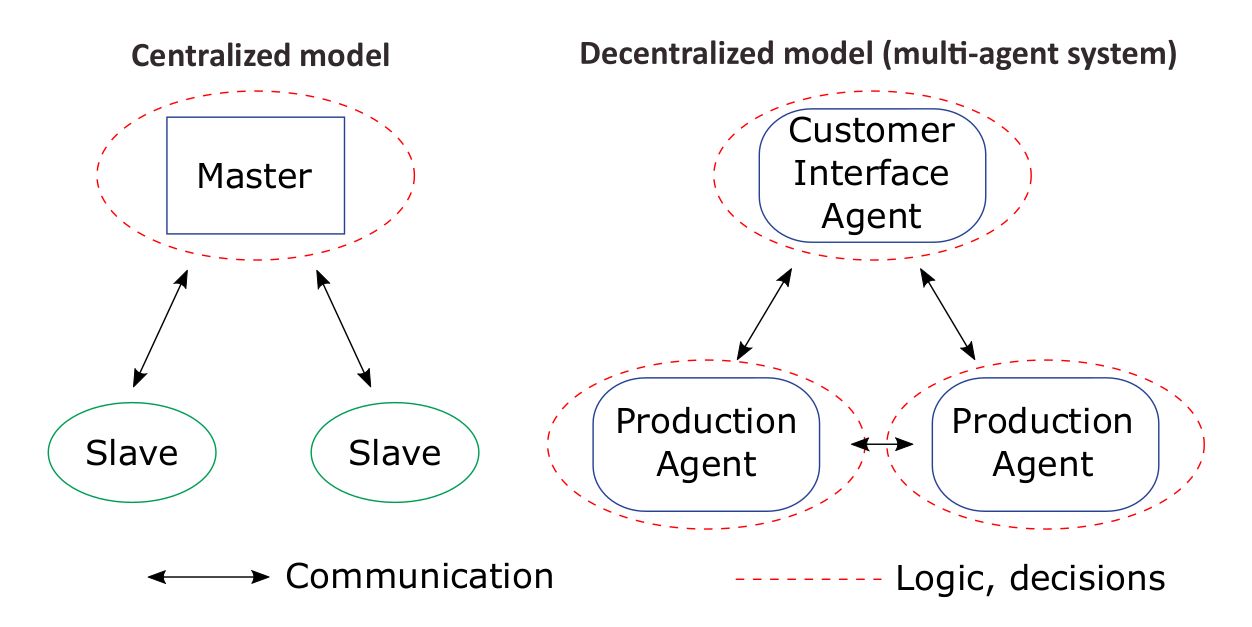
\includegraphics[width=0.8\textwidth]{figures/State-of-the-art/CentralizeDecentralizeConcept.png}

    \caption{Centralized vs. decentralized control schemes compared. 
    In the centralized model, decisions are made only within the 
    master, whereas in the decentralized model, decisions are taken 
    within local resources dependent on both local events or measurements 
    and information exchange with other resources. 
    Source: \cite[fig.1]{egger_deployment-friendly_2020}\label{fig: CentralizeDecentralizeConcept}}
\end{figure}



\section{MAS}

Within the subfields of \gls{mas}, an agent can be identified as a 
software agent with no physical embodiment but only software to control 
physical assets for different purposes. \textit{"In agent-oriented software 
development, an agent is a delineable software unit with a defined goal. 
An agent tries to achieve this goal through autonomous behavior, 
continuously interacting with its environment and other agents"}\cite{wagner_agentenunterstutztes_2008}. 
However, although not under discussion in this thesis, another 
interpretation of \gls{mas} can be a Multi-agent robot system that 
each agent represents an actual physical object, such as an individual 
robot that participates in the complex task execution\cite{ota_multi-agent_2006}.   


Defining \gls{mas} can be confusing, as different researchers approach 
it from various aspects. For a more unambiguous interpretation of the 
concept, a general \gls{mas} can be divided into three views: the 
technical system that comprises robots, the automation control system 
characterized by sensors, actuators, networks, and robot control units, 
and the technical process that describes the production process of the 
product\cite{lauber_prozessautomatisierung_1999}\cite{wannagat_agent_nodate}. 
The focus of this thesis is mainly on the technical system, which can 
be interpreted as a union of robots in a smart factory, with less 
emphasis on the components or functions executed by each robot for 
a specific movement.

For further discretization of an agent, whether the agent is product, 
process, or resource-oriented, an appropriate agent architecture should 
be chosen according to different considerations. There are several of 
them that should be emphasized: \gls{ra}, \gls{ca}, and \gls{ams}. 
\gls{ra} is an agent at the field level representing a single robot. 
Different from the other agents, \gls{ra} should be able to combine 
the modules with physical entities by choosing an appropriate design 
pattern. Therefore, comparing design patterns in different production 
levels is done\cite{ocker_leveraging_2021}. The choice of an ideal 
design pattern should be limited for \gls{ra} in this research by 
comparing three relevant design patterns:  \gls{ra} pattern in Wannagat’s 
architecture, \gls{mfs} patterns in Fischer’s architecture and 
self*-control 
MAS in Ryashentseva’s architecture. Among all,  Wannagat’s architecture\cite{cruz_salazar_cyber-physical_2019} 
is chosen as the appropriate design pattern for \gls{ra} for field level 
control, which consists of five modules: Planning Module, Knowledge Base, 
Control Module, Diagnosis Module, and communication interface. 
All modules are interconnected, meanwhile, with each bound to 
I/Os of a physical system and a communication interface to interact 
with other \gls{ras} or \gls{ams} through \gls{ca} \cite{cruz_salazar_cyber-physical_2019}. 
\gls{ams} and \gls{ca} should have different specifications in the 
same design pattern. \gls{ca}, for example, should be able to coordinate 
the message-based communication between the agents as a "mailbox" 
between them. In contrast, \gls{ams} plays an important role in the 
centralization and coordination of all other agents \cite{wannagat_entwicklung_2010}. 
\begin{figure}[htb]
    \centering
    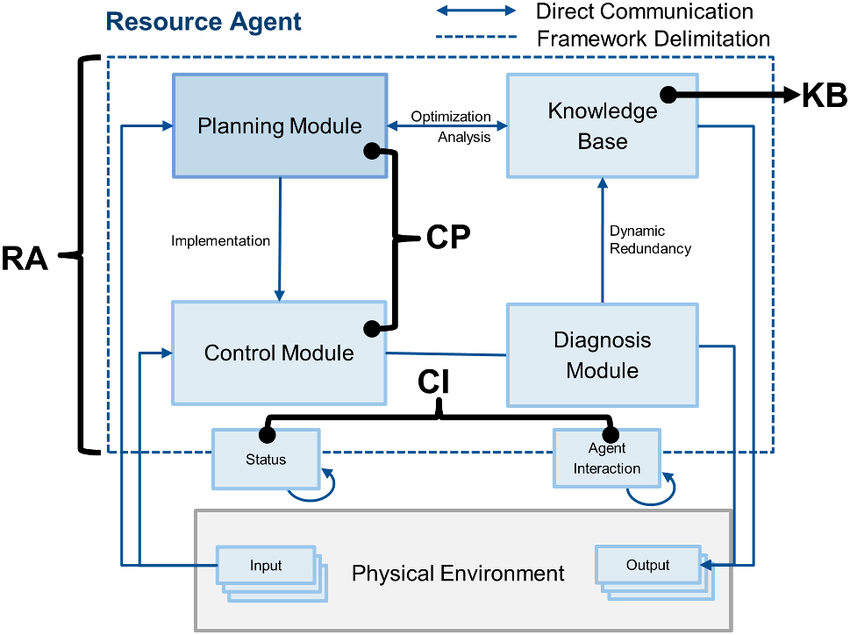
\includegraphics[width=0.8\textwidth]{figures/State-of-the-art/Wannagats-RA-pattern.png}

    \caption{Wannagat's \gls{ra} architecture.
    Source: \cite[fig.1]{cruz_salazar_cyber-physical_2019}\label{fig: Wannagat RA}}
\end{figure}



\section{Network communication}
According to early studies on network delays, the \gls{rtt} and \gls{owd} 
can either be measured by end-to-end methods or estimated with modeling 
approaches. Experiments have led to the consideration that \gls{tcp}-based 
measurements offer a practical solution for evaluating the movement of 
packets from end to end, along with a high packet retransmission rate 
to avoid packet loss\cite{paxson_end--end_1999}. Benefits from 
the development of the internet latency test tools, \gls{tcp} delay 
performance can be evaluated by one of them. Wireshark, for example, is famous 
for capturing network delay in the transport layer, where \gls{tcp} delay 
can be filtered in real-time\cite{dsouza_transmission_2020}. Besides, 
application and presentation layer delays can also be measured by Wireshark and 
other program-specific profiling tools\cite{heger_application_2017}. Furthermore, 
traceroute or ping can be utilized 
for network layer delay collections along with the router logs\cite{Deri2003}. 
Finally, it will be challenging to measure 
data link and physical layer delays, which can be either tracked by hardware 
such as \gls{nic} or calculated based on the characteristics 
of the physical medium. The work of \cite{Fezeu2023}, for example, 
presents a comprehensive, 
in-depth measurement study of mmWave 5G latency performance on the physical layer 
based on a commercial 5G tool.   
Certainly, there are also other tools designed for research for a more 
precise and academic-oriented purpose. In the work of performance testing 
of a 5G campus network, \gls{ftt} designed by ifak Magdeburg was used 
for performance analysis of industrial communication networks\cite{cainelli_performance_2023}, 
with its results later compared with those in this article.


On top of the measured delay 
that includes additional connection establishment and process time, 
models can be built additionally to estimate delays over different layers in 
\gls{osi} model to bridge the gap between experiments and simulations. 
Studies including those for instance the modeling of \gls{tcp}-based 
packet transmission latency that enables both short and 
long \gls{tcp} flows\cite{luan_estimating_2019}. In the book \cite{wehrle2010modeling}, 
both lower and higher-layer wireless modeling tools and methods are introduced. 
Accordingly, common tools and methods for network simulation are ns-3 Network Simulator, OMNeT++, 
IKR Simulation Library and Open WNS. For the lower layer modeling, accurate simulation 
of physical layers can be operated, with the packet domain physical layer simulation 
model given as an example. Another lower-layer modeling approach should be focused on 
link layers, including \gls{mac} and logical link control. As for the higher layer 
modeling, modeling of the network layer and routing protocols, modeling 
transport layer protocols, and the modeling of application traffic are described. 
The combination of lower and higher layers results in the discrete modeling 
of the \gls{osi} model, with their performances tested in different use cases. 




By comparing both estimated and measured delays, a number of insightful 
conclusions made and the corresponding actions can be taken to improve 
the network design.
In the related work for delay measurement of \gls{mas}, 
a comparison between actual and modeling 
delays has been performed\cite{vogel-heuser_delay_2023}, which leads to the 
consideration of integrating \gls{dsl} as further development methods.





\section{\gls{dsl}}
To analyze and optimize the network communication performance, a deeper 
inspection of the network latency is needed. \gls{dsl} has, so far, reached 
some improvements in simplifying the design, presentation, and execution of 
network performance testing for many applications, including server-client applications 
based on hand-coded C, which minimizes the overhead produced by the compiler by 
comparing C and the designed \gls{dsl} based toolset under worst-case scenarios.
A level higher will be the agent-based \gls{dsl} that also includes network-based 
agent communication. The consideration of designing a \gls{dsl} framework 
for the agent's development has been discussed\cite{judith_domain_2013}. Another 
research for fulfilling real-time requirements for safety-critical and 
security-critical engineering has also adapted the \gls{dsl}, which aims to 
modularize the whole \gls{iot} system into a four-level architecture\cite{sklyar_domain_2022}. 



Another notable field for \gls{dsl} is the robotics. Unlike being widely 
used in industrial automation for modeling hard real-time constraints with 
a set of symbols that capture delays from networks and devices, I/O interfaces, 
and industrial controllers\cite{hujo_toward_2022}, \gls{dsl} for robotics is still 
under development due to its higher level of complexity and flexibility in 
robot control. Most of the time, a network communication system is integrated into a group 
of robot operations. To bridge the gap between the highly modularized automation system 
and robotic system, \gls{dsl4ras} for the software and hardware 
properties of robotic drive components are to be defined to meet the need 
of developing a robot-like system based on \gls{dsl}. In the recent work\cite{vogel-heuser_delay_2023}, 
the adaptation of \gls{dsl} is even more straightforward by adopting and 
extending the graphical notations 
from \cite{hujo_toward_2022} and \cite{volpert_supporting_nodate}. It, however, 
leaves the space for further extension. 



The starting point of a requirements-specific \gls{dsl} design is usually 
the existing software. 
A large amount of \gls{dsl} based visualization tools are mostly developed 
to be applied to an open-source robotics middleware suite such as \gls{ros}. 
For example, \gls{rviz} is a \gls{dsl} based 3D 
visualization tool for \gls{ros} that can visualize the robot model and 
capture sensor/actuator information. Movelt, also designed for \gls{ros}, 
provides a set of visual notations that represent the robot kinematics, 
motion planning, and many more. It also allows users to capture the 
timing behaviors of the bounding I/Os. Other middleware tools have been 
developed, but most are hardware and software-dependent. RobotML, a 
Robotic Modeling Language is designed for cross-platform robotic 
software development\cite{hutchison_robotml_2012}. It is developed 
based on Port and Connector to
capture the concept of an interaction between robot systems, including 
Robot, SensorSystem, ActuatorSystem, and LocalizationSystem, with its toolchain 
provided\cite[fig.5]{hutchison_robotml_2012}.



\section{\gls{dt}}


As mentioned earlier in chapter \ref{chap: Motivation}, 
\gls{dt} is a digital mapping of physical entities. Being a rather new concept to 
industrial automation systems, \gls{dt} has gained a lot of attention as a key concept 
of Industry 4.0. According to the existing research on \gls{dt}, their 
directions can be roughly divided into the following categories. The first one 
focuses on the real-time monitoring and visualization of physical assets or systems. 
A \gls{dt} visualization architecture for \gls{fms} has been designed to present 
the high-value information for lifecycle planning, design, debugging, and service 
stages by\cite{fan_digital-twin_2021}. In some cases, the visualization of \gls{dt} 
can be presented in a way for \gls{hmi}\cite{schroeder_visualising_2016}. 


The next orientation of \gls{dt} includes data analytics to support 
learning and decision-making. In a case study of wind power, the data from 
a \gls{dt} model is taken to feed both the physics-based and 
machine learning models\cite{erikstad_merging_nodate}. The processed 
data will be then either stored in a \gls{db} or presented in a regression model. 
Another exemplary \gls{dt} design that has contributed rich functionalities to 
data analytics is the \gls{imt} \gls{dt}\cite{tong_real-time_2020}. 
It contains a data analysis module 
that includes algorithms for error estimation, trajectory kinematics/dynamics 
transformation, machining vibration modal analysis, and a cutting force
estimation.

Based on the data analysis model, predictions can be made to handle failures and 
optimize resources. In \cite{katalinic_digital_2018}, known models are used to solve static and dynamic 
diagnostics tasks and the application for technical process optimization. To fill the 
gaps in maintainence prediction utilizing \gls{dt} big data analytics, a framework 
is designed to support the sharing of data, knowledge, and resources, with a 
mathematical programming model integrated\cite{mi_prediction_2021}. 


The last biggest challenge for \gls{dt} development will be the security threats. 
Although it benefits from breaking the edges in Industry 4.0, industrial stakeholders 
become more and more conservative. The threats exist but are not limited to the following 
fields: software attack, Privilege escalation, Man-in-the-middle, Rogue \gls{dt} 
servers and infrastructures and DT service tampering. Some possible solutions to these 
threats have been introduced, including the improvement of Identity, Authentication 
and Authorization, 
Hardware and Software Security, Hardening of DT Infrastructures and Decoupling, and many 
more. The gain of trust-worthy technologies to overcome security issues will certainly 
gain the confidence of potential \gls{dt} users. 



Our studies for the \gls{dt} part are based on the 
former work for this 
project, which has already provided a foundation for the \gls{dt} 
structure\cite{hofgen_architecture_2023}. 
The work mainly focuses on the realization of an \gls{aas} based Azure \gls{dt} system, 
with an automated \gls{dt} creation and socket-based communication between 
different layers from the \gls{dt} architecture reference 
model\cite[fig.5]{aheleroff_digital_2021}. In our work, the functionalities of \gls{dt} 
will be further investigated with an additional agent-based consideration. 



\section{Real-time requirements for \gls{mas} and \gls{dt}}
Throughout our research, the real-time capability is an important metric for connecting 
various systems and components in \gls{cps}. However, it is not easy to define the 
real-time requirements, which vary greatly due to the system's complexity, 
system interaction requirements, hardware capability, and network latency, 
along with others. 
A use case based real-time requirements for low latency and high reliability 
is defined by\cite{li_5g_2018}, with the floor-level end-to-end latency 
approximately ranging from 1 to 10ms, and the remote control with about 50ms for a 5G 
system. However, according to\cite{zhang_infrastructure_2017}, the real-time 
\gls{qos} requirements for cloud applications (e.g.,\gls{ms} Azure and Amazon Web Service) 
could be selected by a real-time \gls{qos}-aware multicriteria decision-making 
technique. From the paper, an example is given in the gaming industry that has 
high real-time streaming requirements. Hence, the real-time requirement is not unique, and the decision-making for hard or 
soft real-time requirements should be executed in the design stage. 

\section{Research gap}

According to current research, there are various implementations of \gls{mas} in 
different fields. However, there have been limited efforts to standardize and 
modularize the \gls{mas}. In addition, a cloud-based resource digitization should also 
be considered and implemented in the \gls{mas}. In general, the \gls{mas} should be designed 
with a high level of modularization based on \gls{dsl}.

%
% !TeX spellcheck = en_US
\chapter{Methodology}\label{chap: Meth}%
This chapter describes the methodologies of the general \gls{mas} design. 
The general \gls{mas} is distributed into two parts: internal (section \ref{chap: Meth-Internal}) 
and external (section \ref{chap: Meth-External}).  
The internal system includes a \gls{mas} for the \gls{cda} and \gls{ra}, 
while the external system involves the \gls{dta}. 
Although these two systems are decoupled from each other, 
they both follow the principles of an agent-based operating system. 
At the end, it concludes the timing properties for both 
internal and external systems with protocols in 
different layers and suggests a way to represent 
network latency modularly using visual notation of \gls{dsl}.
\section{Internal}\label{chap: Meth-Internal}
This section discusses the selected design pattern for \gls{mas} along 
with the responsibilities of each module within it.
It then compares the features of transport layer protocols with those of 
application layer protocols.
Eventually the methods for using python WebSocket for \gls{mas} and 
RESTful API for one to one agent communication are presented in form of pseudocode. 

\subsection{Overview (conceptual diagram)}

%figure conceptual MAS
\begin{figure}[htb]
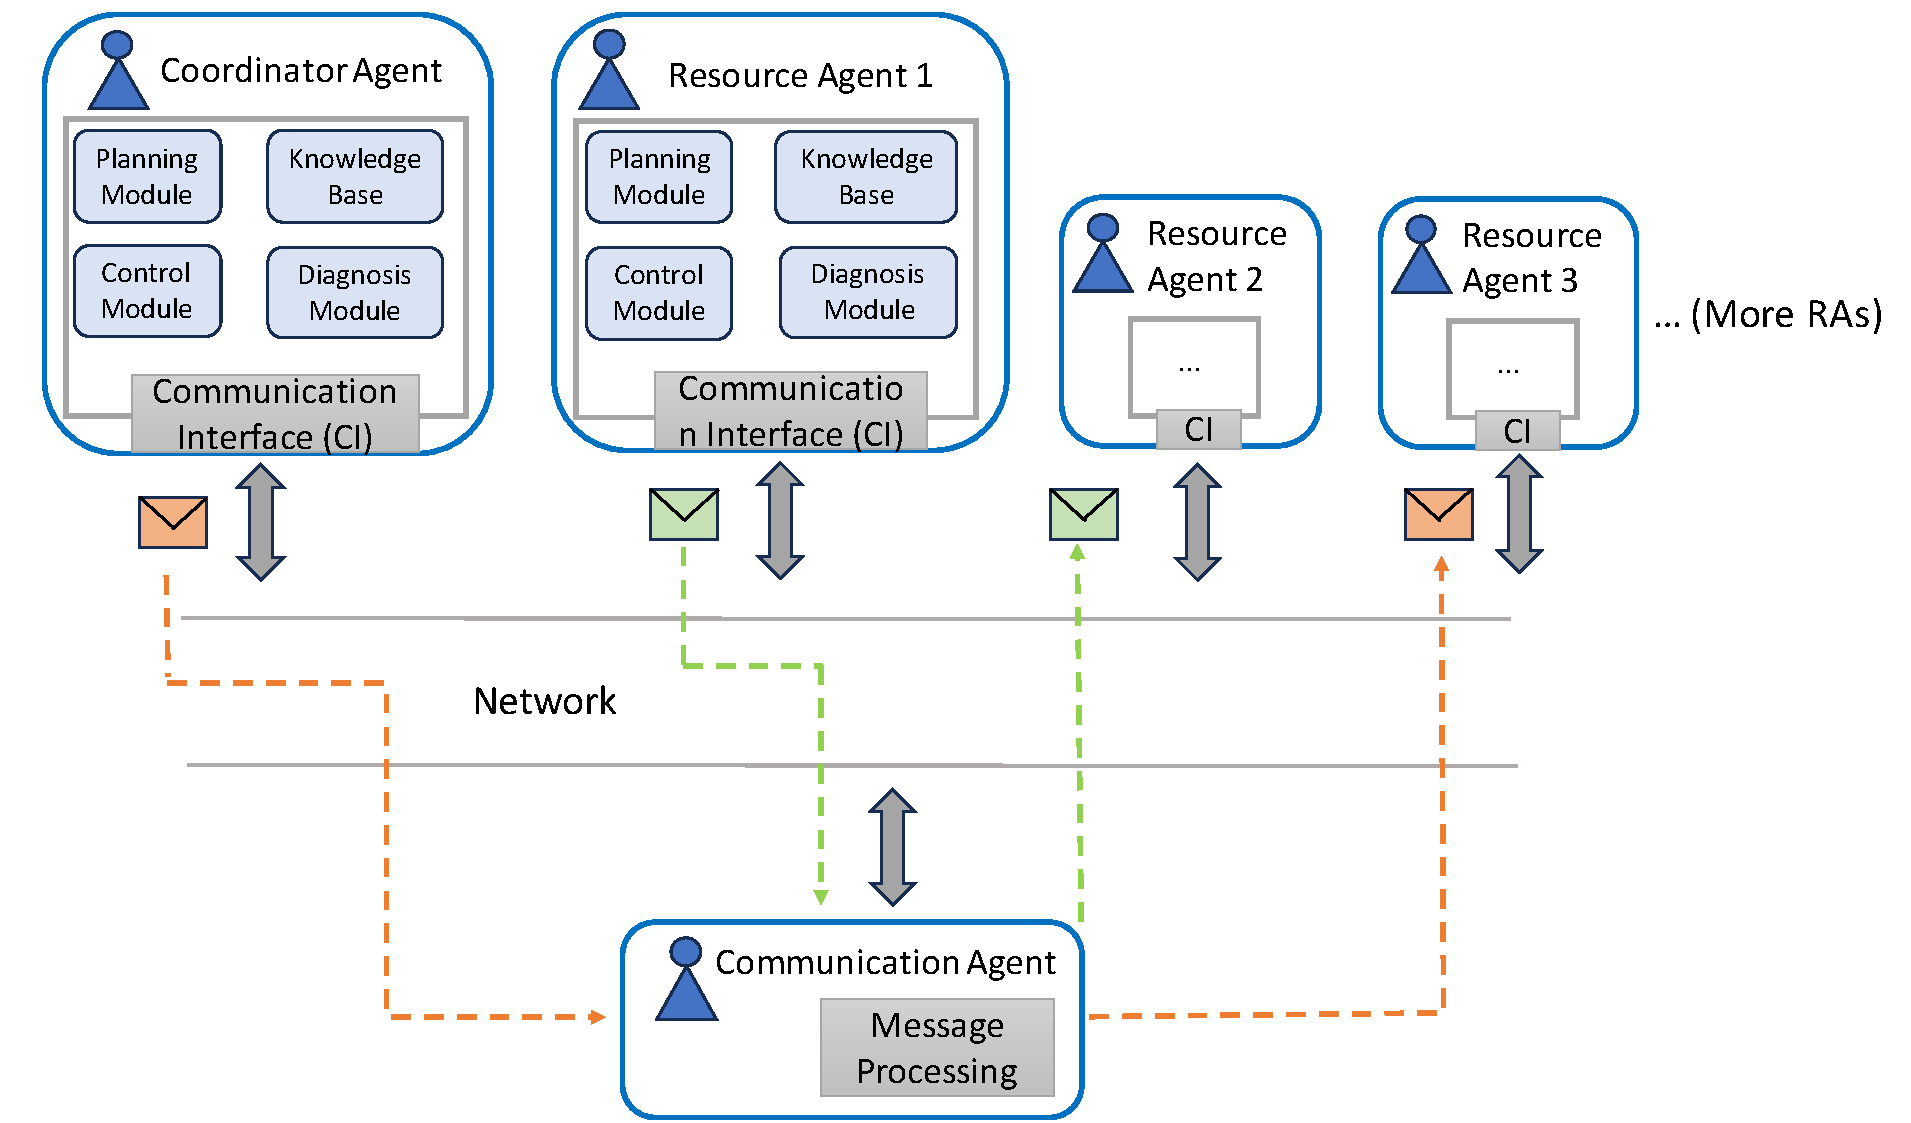
\includegraphics[width=\textwidth]{figures/MAS_Conceptual_Diagram.pdf}
\centering
\caption{Conceptual diagram of MAS\label{fig: MASConceptual}}
\end{figure}

% decribe the conceptual diagram

Fig.\ref{fig: MASConceptual} shows a conceptual diagram of a \gls{mas} based 
on the \gls{ra} design patterns 
in Wannagat’s architecture\cite{cruz_salazar_cyber-physical_2019}, 
focusing on communication between agents, 
planning, and decision-making inside each agent. The \gls{cda} here is identical 
to \gls{ams} of Wannagat’s architecture, which should also be considered an agent 
instead of a management system. The five modules within an agent are:


The five modules within an agent are: 
\begin{itemize}
    \item Planning Module
    \item Control Module
    \item Knowledge Base
    \item Diagnosis Module
    \item Communication Interface
\end{itemize}

for both \gls{cda} and \gls{ra}.
Based on these five modules, the agents executing functions can be categorized into five parts. 
The following tab.\ref{tab:designPatterns} shows 
some functions of each module based on the general requirements of a smart factory.


\begin{table}[p]
    \setlist[itemize]{leftmargin=*, topsep=0pt, itemsep=2pt, parsep=0pt}
    \caption{Wanagat's \gls{ra} design patterns with task related examples.}
    \label{tab:designPatterns}
    \small
    \renewcommand{\arraystretch}{1.2} 
    \setlength{\extrarowheight}{3pt}
    \centering
    \begin{tabularx}{\textwidth}{|Y|Z|W|}
    \hline
    \multicolumn{3}{|c|}{Wanagat's design patterns} \\ 
    \hline
    Module name & Task & Example \\ 
    \hline
    Planning Module &
    \vspace{-10pt}    
    \begin{itemize}
        \item Task planning 
        \item Decision making 
        \item Resource allocation 
        \item Sequencing 
        \item Scheduling
    \end{itemize} 
    &  
    \vspace{-10pt}   
    \begin{itemize}
        \item Break down tasks into smaller executable units
        \item Decide which task should be assigned to which agent 
        \item Allocate the agents with specific tasks 
        \item Find the task execution sequence 
        \item Calculate the execution time for each agent
    \end{itemize} \\
    \hline
    
    Control Module & 
    \vspace{-10pt}
    \begin{itemize}
        \item Monitoring 
        \item Adaptation 
        \item Control and optimization 
        \item Resource allocation 
        \item Actuation
    \end{itemize}
    & 
    \vspace{-10pt}
    \begin{itemize}
        \item Acquisition of robot states
        \item Adapt the plans with current state (e.g., emergent stop) 
        \item Control and optimize the robot's motion 
        \item Allocate the agents with specific tasks 
        \item Actuate the robot with outputs
    \end{itemize} \\
    \hline
    
    Knowledge Base & 
    \vspace{-10pt}
    \begin{itemize}
        \item \gls{db}
        \item Knowledge representation and reasoning 
        \item Learning 
        \item Knowledge sharing 
    \end{itemize}
    & 
    \vspace{-10pt}
    \begin{itemize}
        \item Hierarchical, relational, non-relational and object oriented
        \item Relational ontology \gls{db} system
        \item Agent learns from the existing primitives and create new executable primitives for customer's changing requirements
        \item Unfound primitives could be retrieved by querying other agents
    \end{itemize} \\
    \hline

    Diagnosis Module & 
    \vspace{-10pt}
    \begin{itemize}
        \item Fault detection 
        \item Fault diagnosis 
        \item Fault prediction 
        \item Root cause analysis and classification
    \end{itemize}
    & 
    \vspace{-10pt}
    \begin{itemize}
        \item Hierarchical, relational, non-relational and object oriented
        \item Relational ontology \gls{db} system
        \item Agent learns from the existing primitives and create new executable primitives for customer's changing requirements
        \item Unfound primitives could be retrieved by querying other agents
    \end{itemize} \\
    \hline

    Communication Interface & 
    \vspace{-15pt}
    \begin{itemize}
        \item Message parsing and encoding
        \item Connection establishment, maintenance
        \item Message handling 
        \item Data security
    \end{itemize}
    & 
    \vspace{-15pt}
    \begin{itemize}
        \item Encode and decode the massages in agent specific data type, or  parse the data object to other types (e.g., json)
        \item Ensure the connection with other agents based on system requirements
        \item Filter messages with undesired data type or incomplete messages, prioritize the incoming messages
        \item Ensure data integrity and confidentiality by encrypting, decrypting and authenticating messages
    \end{itemize} \\
    \hline
    \end{tabularx}
    \end{table}


\subsection{Prerequisite}
\subsubsection{System Setup}
 
%figure conceptual MAS
\begin{figure}[htbp]
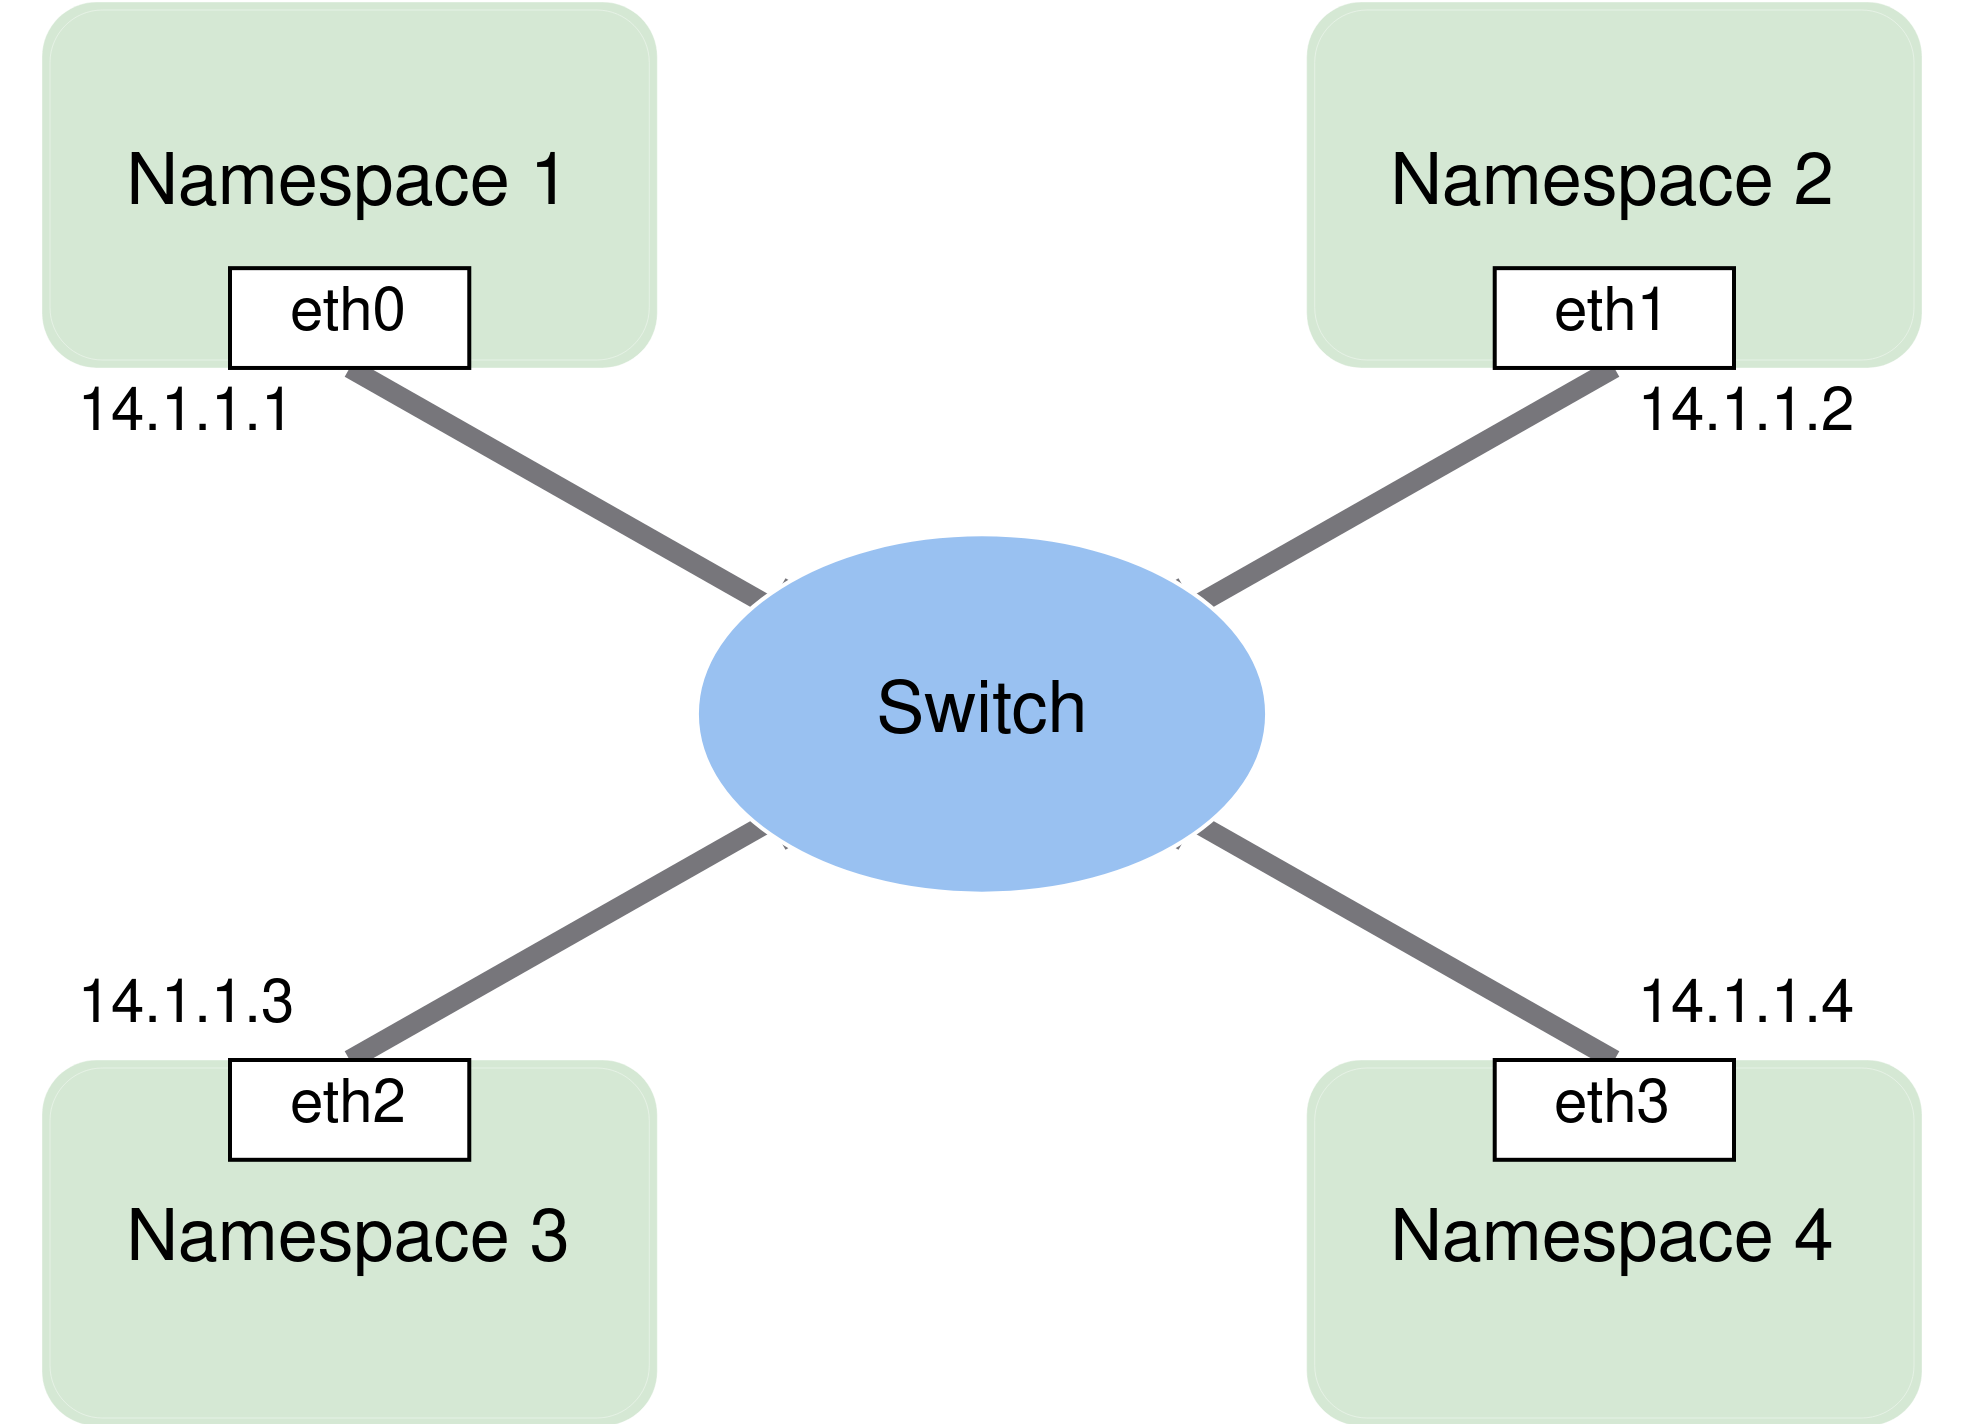
\includegraphics[width=0.8\textwidth]{figures/NamespaceConceptual.png}
\centering
\caption{Conceptual diagram of namespaces creation
\label{fig: NSConceptual}}
\end{figure}


Before simulating network environments for agent communication testing 
and development of the \gls{mas}, the internal packet routing between agents 
in a single Linux device should be avoided. A common way to visualize 
the network for performance testing is to use namespaces for network 
emulation. The trick is that a process running within a given
namespace will see only the network interfaces, including, for example, 
virtual interfaces and forwarding tables, that exist in that namespace. 
The applications under test should serve as a
switch, and each packet should be routed through these interfaces. 
Fig.\ref{fig: NSConceptual} shows that each namespace is assigned 
a virtual ethernet interface, 
starting with the name eth, along with an individual IP address. 
Each time a script gets called, it runs under a namespace with its 
IP address. In exercise, if a packet is sent from
Namespace 1 to 3 and then back; it is routed by the switch instead of 
bridges between namespaces to avoid internal routing.

\subsection{\gls{osi} model and comparison between sockets relevant protocol layers}
%figure conceptual MAS
\begin{figure}[htbp]
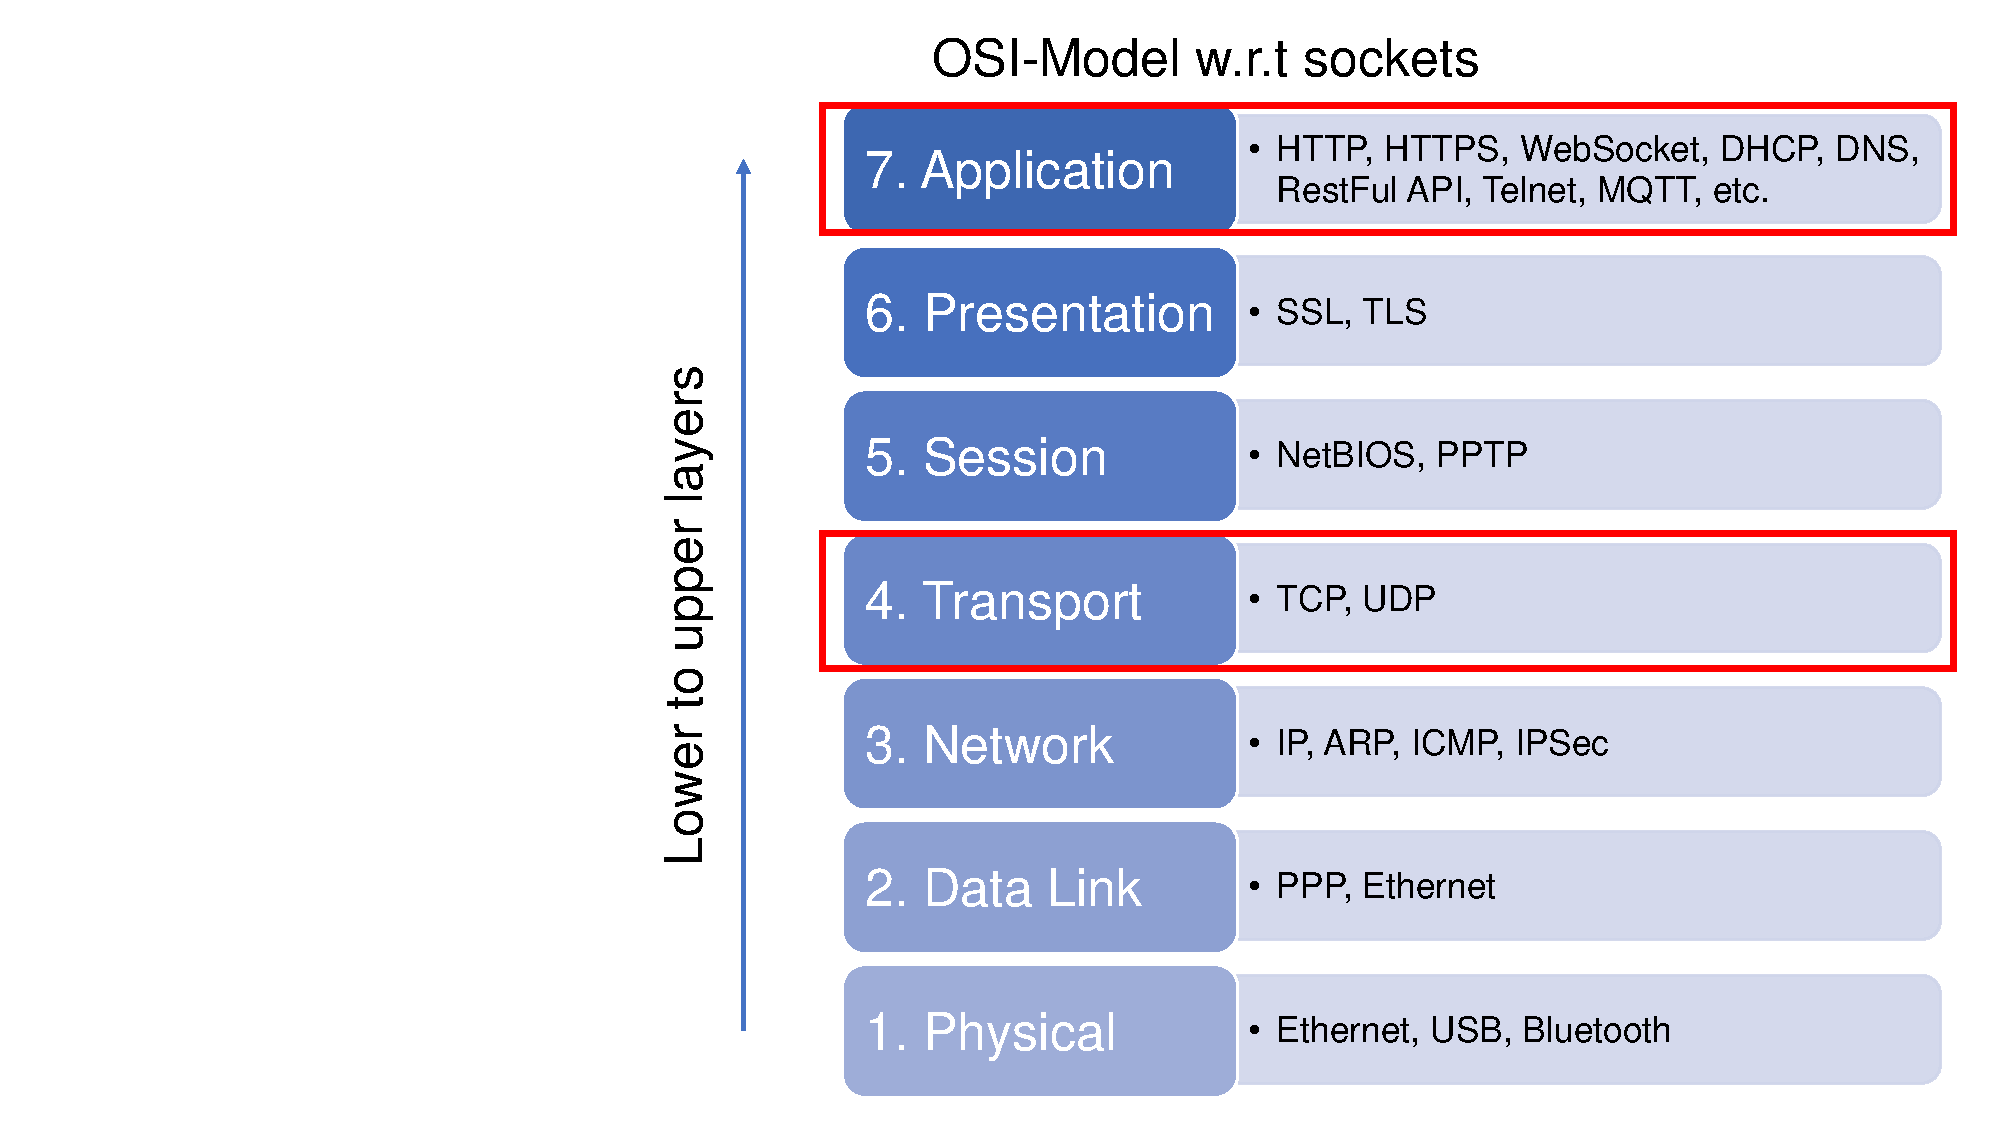
\includegraphics[width=0.8\textwidth]{figures/OSI.pdf}
\centering
\caption{\gls{osi} model with example protocols \label{fig: OSI}}
\end{figure}



Fig.\ref{fig: OSI} shows the famous OSI model with seven abstraction layers, with Transport and 
application layers most relevant to sockets. TCP and UDP are typical transport layer 
protocols, and they provide a mode of end-to-end data transport between two devices, 
while the application layer protocols like HTTP or Websocket establish communication 
between applications within devices. Although the application layer protocols still 
utilize TCP/UDP sockets to transport stream data, they defined additional "rules" to 
specify the structure, content, and semantics of the messages transported through 
sockets. In the following tables, a comparison
between protocols in different layers provide a more straightforward overview of 
their pro and cons in different contents.



\subsubsection{Transport layer protocols}

Tab.\ref{tab: transportlayer} compares the typical transport layer protocols \gls{tcp} 
and \gls{udp} from different aspects. \gls{tcp} provides reliable data 
transport, while \gls{udp} mainly focuses on transport speed and efficiency without a 
reliability guarantee. With a focus on speed and reliability, UDP, on the one hand, 
offers faster packet
transport. On the other hand, it produces a network-dependent packet loss rate and 
out-of-order packet sequence compared to TCP. Because of the requirement of a 
reliable real-time ordered data transport with minimum to no packet loss in \gls{mas} 
communication, \gls{tcp} is used as the base protocol of the design.

\begin{table}[htbp]
    \small
    \centering
    \caption{Characteristics of different technologies in transport layer protocols}
    \label{tab: transportlayer}
    \begin{tabular}{|m{0.2\textwidth}|m{0.3\textwidth}|m{0.3\textwidth}|}
    \hline
    \multicolumn{3}{|c|}{\textbf{Transport layer protocols}}                                                            \\ \hline
    \textbf{Aspect}                         & \textbf{\gls{tcp}}             & \textbf{\gls{udp}}        \\ \hline
    Use cases                      & Web browsing, email, text messaging, and file transfers & Live and real-time data transmission \\ \hline
    Reliability                    & Reliable        & Unreliable \\ \hline
    Stream type                    & Byte stream with no preserved boundaries & Message stream with preserved boundaries \\ \hline
    Connection type                & Connection oriented, three handshake & No connection needed \\ \hline
    Overhead                       & Larger than \gls{udp} & Very low   \\ \hline
    Sequence                       & Packets arrive in sequence & No sequencing for packets \\ \hline
    Retransmission of lost packets & Yes             & No         \\ \hline
    Speed                          & Slower than \gls{udp}, because of overhead and connection & Relative faster than \gls{tcp} \\ \hline
    State                          & Stateful        & Stateless  \\ \hline
    Flow control                   & Yes             & No         \\ \hline
    \end{tabular}
\end{table}




\subsubsection{Application layer protocols}


% % Please add the following required packages to your document preamble:

\begin{sidewaystable}[p]
    \small
    \caption{Characteristics of different technologies in application layer protocols}
    \label{tab: applicationlayer}
    \centering
    \begin{tabular}{|m{0.15\textwidth}|m{0.25\textwidth}|m{0.25\textwidth}|m{0.25\textwidth}|}
    \hline
    \multicolumn{4}{|c|}{\textbf{Application layer protocols}} \\ \hline
    \textbf{Aspect} & \textbf{HTTP} & \textbf{WebSocket}  & \textbf{MQTT} \\ \hline
    Use cases & Web pages, images, videos, World Wide Web, etc & Such as chat applications, live gaming, etc & Usually in IoT with limited bandwidth \\ \hline
    Functionality & Request-response protocol based on TCP, foundation for both RESTful APIs and the initial connection in WebSockets & Bi-directional, real-time communication & Lightweight message transport, runs over TCP \\ \hline
    Security & Use SSL/TLS & ws (unsecured) and wss (secured with SSL/TLS) & Use TLS, like username/password authentication and optional message-level security \\ \hline
    Message patterns & Request-Response & Full Duplex (send and receive independent) & Publish-Subscribe \\ \hline
    Connection type & No connection needed & Persistent {connection} & Persistent connection \\ \hline
    State & Stateless & Stateful & Stateful \\ \hline
    Overhead & Overhead for each request-response cycle, especially for new connections & After the initial handshake (HTTP), data frames are lightweight & Minimal message overhead \\ \hline
    Realtime capability & Less Capable & Highly Suitable & Highly Suitable \\ \hline
    Flexibility & Supported in all environments & Supported in most modern web browsers and many backend environments & Highly flexible \\ \hline
    Adaptability to dynamic changes & Relative lower (influenced by stateless nature) & High & High \\ \hline
    Capability of handling instability & Less capable, requires a stable connection for each request-response cycle & Less stable if connection disruptions happen frequently & Capable, Ideal for remote locations with limited connectivity \\ \hline
    Scalability & Less scalable, require more infrastructure support & Highly scalable, maintains connections for real-time interactions & Highly scalable based on broker-client message transport \\ \hline
    \end{tabular}
\end{sidewaystable}

Several protocols in application layers are considered suitable for \gls{mas} 
communication, each with advantages and limits in different aspects according to 
ab.\ref{tab: applicationlayer}.
To get a closer look at the tab.\ref{tab: applicationlayer}, a horizontal comparison 
between different application layer protocols: 


\begin{itemize}
    \item \gls{http}
    \item WebSocket
    \item and \gls{mqtt}
\end{itemize}

should be performed. In one word, WebSocket is chosen to be the application 
layer protocol for MAS communication, while \gls{tcp} socket for the \gls{dta} 
design, which will be further discussed in the next chapter. Here are the 
reasons for the choice of WebSocket: 


\begin{itemize}
    \item Bi-directional, full-duplex, real-time communication between server and clients, no re-connection needed, suitable for continuous data transport
    \item Small overhead after connection establishment to reduce latency (\gls{http})
    \item Stateful, store the information of the client's state under connection
    \item High flexibility, adaptability and scalability
    \item Secure with wss
\end{itemize}

Fig.\ref{fig: MsgConceptual} illustrates the differences between bi-directional full-duplex and other message patterns, such as Request-Response and Publish-Subscribe, in the context of data transport.
For the \gls{mqtt}, the publisher publishes (sends) a message within a topic to the broker (server), while the subscriber subscribes (receives) the message from the broker within the same topic. 
For response, a new topic needs to start, but there is no guarantee that the original publisher is listening, which is a drawback for send-and-receive patterns of \gls{mas}. 

Out of the four protocols, the other three are considered more appropriate. One such protocol is HTTP, which operates on a request-response mechanism. In this mechanism, a client sends messages to the server, and the other client receives them. Regardless of the success of the GET and POST methods, a response is always provided. For each message that goes through the server, a new connection is established, and it is closed after the responses are sent.
The inconsistent connection will consume more communication time and lead to higher latency. 
The WebSocket protocol, on the other hand, provides bi-directional and full duplex real-time communication, minimizing communication delays caused by inconsistent connections.
The client sends a message to the server. After processing the data, the server will pass the message to the other client and receive a response with the same logic, which allows simultaneous communication in both directions between clients so that no re-connection in the message transport cycle is necessary. The consistent server-client connection makes it possible to realize continuous real-time communication between agents. In the next section, a more detailed explanation of the WebSocket mechanism for \gls{mas} design will be given.
%figure conceptual application layer protocols
\begin{figure}[htb]
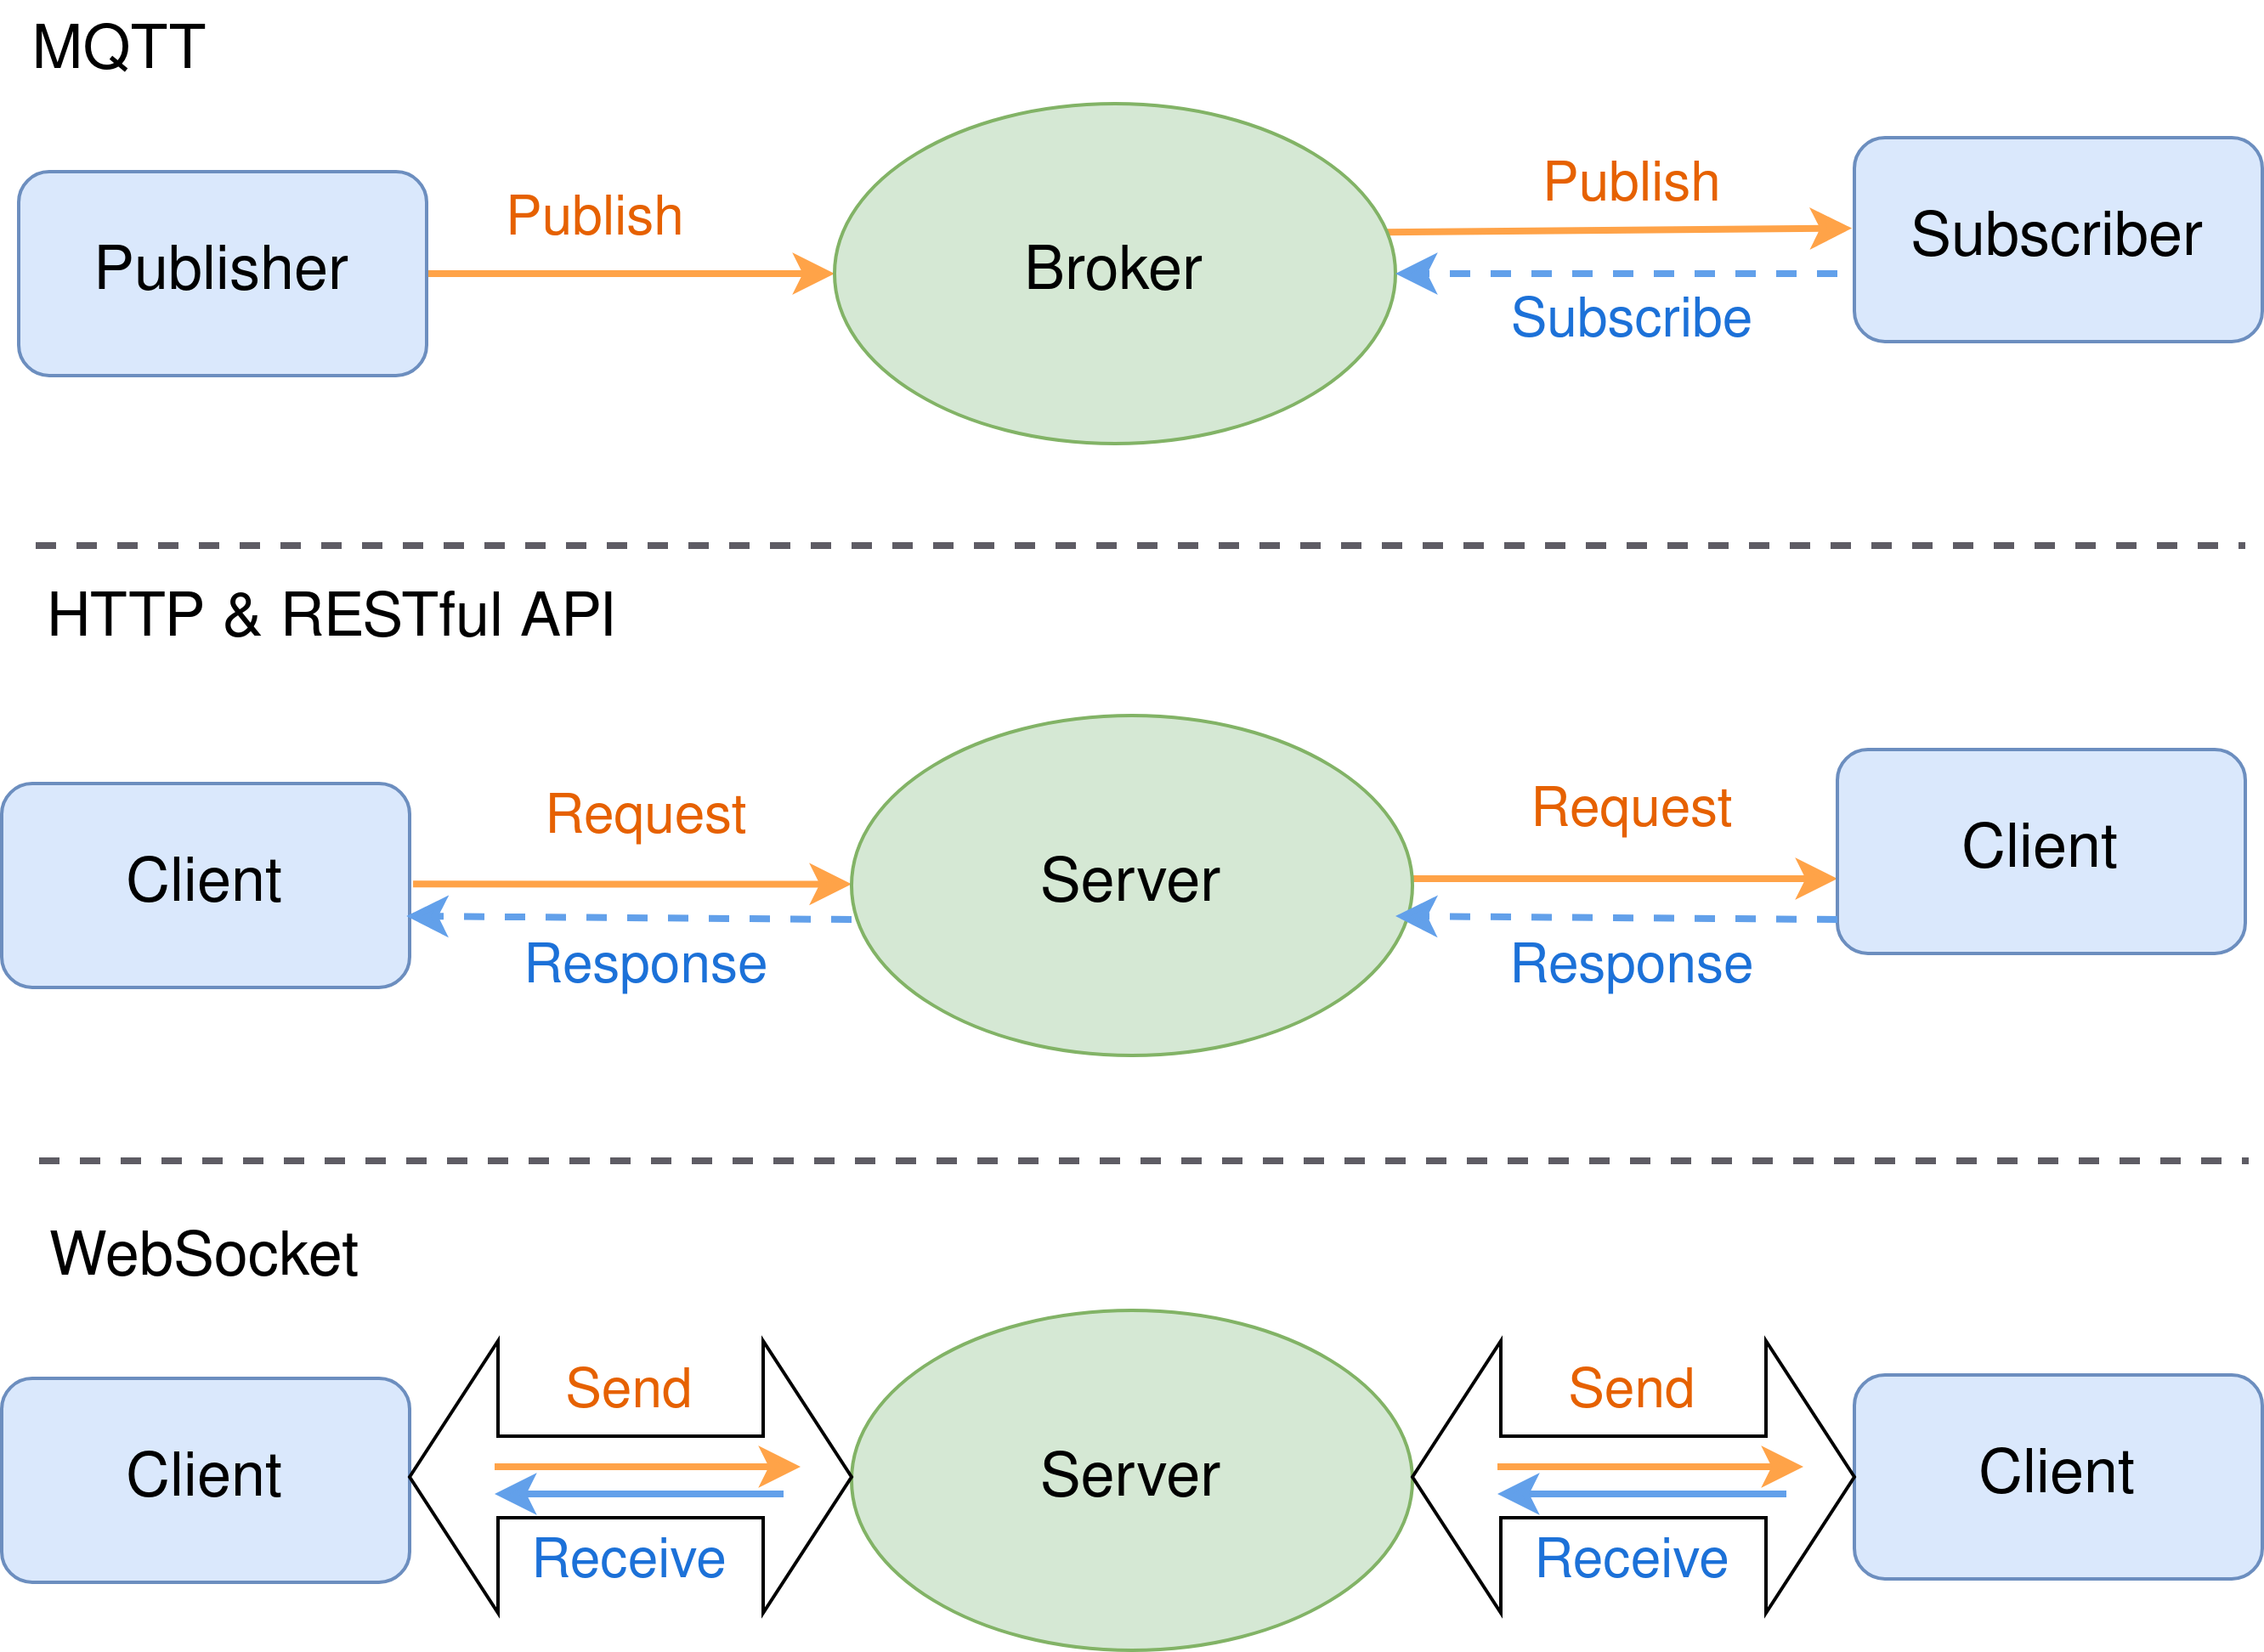
\includegraphics[width=0.8\textwidth]{figures/MessageConceptual.png}
\centering
\caption{Conceptual diagram of different applcation layer 
protocols\label{fig: MsgConceptual}}
\end{figure}

\subsection{Transport layer protocols versus Application layer protocols}
The reasons of choosing application layer protocols over transport layer protocols for \gls{mas} according to tab.\ref{tab: transportlayer} and \ref{tab: applicationlayer} are listed as following:
\begin{itemize}
    \item Semantic-rich message patterns
    \item Higher flexibility
    \item Standardized communication between different agents
    \item Header with agent relevant information
    \item Security and authentication
    \end{itemize}
However, unlike for \gls{mas} design, the architecture of \gls{dta} is more straightforward and the basic \gls{tcp} socket is chosen for the more to one server-client communication. 
The details will be discussed later in section \ref{chap: Meth-External}.

\subsection{Pseudo-Code of MAS workflow in WebSocket python}\label{chap: Meth-WS-MAS}
In algorithm \ref{alg: CDAPseudoCode} is a piece of pseudocode that reflects the workflow of the \gls{mas} for the \gls{cda}. 
Unlike other \gls{ras}, \gls{cda} has no mechanisms of primitive execution but the ability to do planning and decision-making. 
Under the Main, the production tasks are broken down into a list of sequenced primitives and then assigned to each allocated agent through one of the predefined $send\_and\_receive()$ functions under the messageSender class.
After getting responses from the agents, \gls{cda} should decide whether to start processing positive responses or retry the steps by negative responses.  
Once the production process starts, the \gls{cda} assumes the role of a coordinator and waits for inform messages from the allocated agents. It does so by using one of the $receive\_and\_send()$ functions under the messageReceiver class. This allows the \gls{cda} to have overall control of the entire production process and centralize the distributed agent systems.


As for the decentralization of \gls{mas}, the \gls{ra} should be able to react to \gls{cda} and do the decision-making for its field-level control, which means \gls{cda} should only be informed about the status of the production process. In contrast, the exact processes should be done within \gls{ra}, and the material flow should be informed between \gls{ras}. The combination of centralization and decentralization will save the resource power consumed by \gls{cda}, 
while still maintaining the management level control and decision-making.  
The algorithm \ref{alg: RAPseudoCode} shows the logic of a \gls{ra}. At the beginning, \gls{ra} waits for the connection and capability check from \gls{cda}. After that, the first agent in the list of $sequenced\_agent$ will listen to the starting message from \gls{cda}. 
Moreover, other agents will wait for the availability check and inform messages from the last agent on the list. 
Once the \gls{ra} has completed its own primitives, it should check for the availability of the next agent and inform its starting point. 
Once all primitives in the list are executed, the last agent should inform the \gls{cda} about the end of processing.


Before the agents start to run, the WebSocket server program (algorithm \ref{alg: ServerPseudoCode}) must be started first so that the messages from agents will be routed to it, which serves as a \gls{ca}.  
The server runs asynchronously and listens to incoming messages forever, meaning that every time a new agent gets connected, a new thread will be started and killed after the incoming message is processed and sent to the recipient agent. 
All threads run concurrently, and the hardware limits the maximum possible connection number and also the network bandwidth and latency. 
After the server receives a message, it should identify the message type to check whether it is in JSON or string format. 
After that, it will split the string or parse the JSON file to retrieve the recipient name, the priority, and the message content. 
Since all message-handling processes run concurrently, there is a chance that multiple messages are coming into the server and waiting for processing at the same time. 
In order to rearrange them and handle the messages with higher priority in advance, all messages should be pushed to the queue, and the critical messages should be popped out first. The critical messages have the highest priority, and after this, the important and then the normal messages. 
Finally, the message will be processed further or sent directly to the recipient. 
   
\begin{breakablealgorithm}
\caption{Pseudo-Code for \gls{cda} in MAS workflow}
\label{alg: CDAPseudoCode}
\begin{algorithmic}[1]
\State \textbf{Input:} custRequirement
\State {Import} WebSocket
\State {Initialize} agentID, centralServerIP
\State \textbf{Class} messageSender
    \State \textbf{\qquad function} {$send\_and\_receive(self, recipient, message, priority)$}
    \State \qquad \qquad Establish a WebSocket connection    
    \State \textbf{\qquad \qquad while} recipient not Found \textbf{do}    
    \State \qquad \qquad \qquad Send prioritized messages and wait for response

    \State \textbf{\qquad function} {$send\_capCheck\_and\_receive(self, recipient, primitive, priority)$}
    \State \qquad \qquad Establish a WebSocket connection
    \State \textbf{\qquad \qquad while} recipient not found \textbf{do} 
    \State \qquad \qquad \qquad Send prioritized messages and wait for response
    \State \qquad \qquad \qquad Handle capability exceptions

    \State \textbf{\qquad function} {$send\_image\_and\_receive(self, recipient, image\_path, priority)$}
    \State \qquad \qquad {\#similar to $send\_and\_receive()$ but send an image }    
    % \State \qquad \qquad ...

    \State \textbf{\qquad function} {$send\_availCheck\_and\_receive(self, recipient, primitive, priority)$}
    \State \qquad \qquad {\#similar to $send\_capCheck\_and\_receive()$ but raise availibility exceptions } 
    % \State \qquad \qquad ...

\State \textbf{EndClass}
\State \textbf{Class} messageReceiver
    \State \textbf{\qquad function} {$receive\_and\_send(self, response, priority)$}
    \State \qquad \qquad Establish a WebSocket connection
    \State \textbf{\qquad \qquad while} message not received \textbf{do}
    \State \qquad \qquad \qquad Receive, process and send responses with priority
    \State \textbf{\qquad function} {$receive\_image\_and\_send(self, response, priority)$}
    \State \qquad \qquad {\#similar to $receive\_and\_send()$ but receive and save an image }    
    % \State \qquad \qquad ...    
    \State \textbf{EndClass}
\State \textbf{Class} agentsAllocation
    \State \textbf{\qquad function} {$allocate\_agents\_with\_seq\_primitives(self, requirements)$}
    \State \qquad \qquad Find tasks from customer requirements
    \State \qquad \qquad Breakdown tasks into skills into primitives
    \State \qquad \qquad Create sequence lists for primitives and agents allocation    
    \State \qquad \qquad \textbf{return} sequences
    \State \textbf{EndClass}
\State \textbf{Main:}
\State {\qquad Instantiate} agentsAllocation, messageSender and messageReceiver with agentID
\State \qquad $sequences = allocate\_agents\_with\_seq\_primitives(custRequirement)$
\State \qquad \textbf{repeat}
\State \qquad \qquad $send\_and\_receive(agent, connectMsg, priority)$
\State \qquad \textbf{until} all allocated agents connected
\State \qquad \textbf{repeat}
\State \qquad \qquad $send\_capCheck\_and\_receive(agent, primitive, priority)$
\State \qquad \textbf{until} all allocated agents capable of all primitives
\State \qquad \textbf{repeat}
\State \qquad \qquad $send\_and\_receive(agent, sequences, priority)$
\State \qquad \textbf{until} all allocated agents receive sequences
\State \qquad \qquad $send\_availCheck\_and\_receive(1st\_Agent, 1st\_primitive, priority)$
\State \qquad \textbf{repeat}
\State \qquad \qquad $receive\_and\_send(responseMsg, priority)$
\State \qquad \textbf{until} informed by last agent with finish message 
\State \textbf{End} 
\end{algorithmic}
\end{breakablealgorithm}

%pseudo code for RA
\begin{breakablealgorithm}
    \caption{Pseudo-Code for \gls{ra} in MAS workflow}
    \label{alg: RAPseudoCode}
    \begin{algorithmic}[1]
    \State {Import} WebSocket
    \State {Initialize} agentID, centralServerIP, subServerIP
    
\State \textbf{Class} messageSender
    \State \textbf{\qquad function} {$send\_and\_receive(self, recipient, message, priority)$}
    \State \qquad \qquad Establish a WebSocket connection    
    \State \textbf{\qquad \qquad while} recipient not Found \textbf{do}    
    \State \qquad \qquad \qquad Send prioritized messages and wait for response

    \State \textbf{\qquad function} {$send\_availCheck\_and\_receive(self, recipient, primitive, priority)$}
    \State \qquad \qquad Establish a WebSocket connection
    \State \textbf{\qquad \qquad while} recipient not found \textbf{do} 
    \State \qquad \qquad \qquad Send prioritized messages and wait for response
    \State \qquad \qquad \qquad Handle availability exceptions

    \State \textbf{\qquad function} {$send\_image\_and\_receive(self, recipient, image\_path, priority)$}
    \State \qquad \qquad{\#similar to $send\_and\_receive()$ but send an image }
    % \State \qquad \qquad ...

\State \textbf{EndClass}

\State \textbf{Class} messageReceiver
    \State \textbf{\qquad function} {$receive\_and\_send(self, response, serverID)$}
    \State \qquad \qquad Establish a WebSocket connection
    \State \textbf{\qquad \qquad while} message not received \textbf{do}
    \State \qquad \qquad \qquad Receive, process and send responses with priority
    \State \textbf{\qquad function} {$receive\_capCheck\_and\_send(self, response, serverID)$}
    \State \qquad \qquad Establish a WebSocket connection
    \State \textbf{\qquad \qquad while} message not received \textbf{do}
    \State \qquad \qquad \qquad Receive, check capability and send responses with priority
    \State \qquad \qquad \qquad Handle capability exceptions
    \State \textbf{\qquad function} {$receive\_sequences\_and\_send(self, response, serverID)$}
    \State \qquad \qquad Establish a WebSocket connection
    \State \textbf{\qquad \qquad while} message not received \textbf{do}
    \State \qquad \qquad \qquad Receive, store sequences and send responses with priority

    \State \textbf{\qquad function} {$receive\_image\_and\_send(self, response, serverID)$}
    \State \qquad \qquad{\#similar to $receive\_and\_send()$ but receive and save an image }    
    % \State \qquad \qquad ...    
    \State \textbf{\qquad function} {$receive\_availCheck\_and\_send(self, response, serverID)$}
    \State \qquad \qquad {\#similar to $receive\_capCheck\_and\_send()$ but check availability}
    % \State \qquad \qquad ...  
    \State \textbf{EndClass}
 

   
    \State \textbf{Main:}
    \State {\qquad Instantiate} messageSender and messageReceiver with agentID
    \State \qquad $receive\_and\_send(connectMsg, centralServerID)$
    \State \textbf{\qquad repeat}
    \State \qquad \qquad $receive\_capCheck\_and\_send(capMsg, centralServerID)$
    \State \textbf{\qquad until} CapabilityCheck finished  
    \State \textbf{\qquad for} agent in sequence {\textbf do}
    \State \textbf{\qquad \qquad if} {agent is first in sequence} \textbf{then}
        \State {\qquad \qquad \qquad} $receive\_availCheck\_and\_send(availMsg, centralServerID)$
        \State \textbf{\qquad \qquad else}
        \State \textbf{\qquad \qquad \qquad if} {previous agent is not self} \textbf{then}
            \State \qquad \qquad \qquad \qquad $receive\_availCheck\_and\_send(availMsg, SubServerID)$
            \State \qquad \qquad \qquad \qquad executePrimitive(primitive)
        
            \State \textbf{\qquad \qquad \qquad if} {agent is not last one AND next agent is not self} \textbf{then}
            \State \textbf{\qquad \qquad \qquad \qquad} $send\_availCheck\_and\_receive(nextAgent, primitive, priority)$
            \State \textbf{\qquad \qquad \qquad \qquad} executePrimitive(primitive)
            \State \textbf{\qquad \qquad \qquad \qquad} $send\_and\_receive(nextAgent, informMsg, priority)$
         
            \State \textbf{\qquad \qquad \qquad if} {agent is last} \textbf{then}
            \State \textbf{\qquad \qquad \qquad \qquad} executePrimitive(primitive)
            \State \textbf{\qquad \qquad \qquad \qquad} $send\_and\_receive(\gls{cda}, informFinishMsg, priority)$
            \State \textbf{\qquad end for} 
    \State \textbf{End} 
\end{algorithmic}
\end{breakablealgorithm}


%pseudo code for Server
\begin{breakablealgorithm}
    \caption{Pseudo-Code for \gls{ca} as a server in MAS workflow}
    \label{alg: ServerPseudoCode}
    \begin{algorithmic}[1]
        \State {Import} WebSocket
        \State {Initialize} serverID, priorityDict, messageQueue, connectedAgents
        \State \textbf{Do in parallel}
        \State \textbf{\qquad function} handler(WebSocket, path)  
        \State \textbf \qquad \qquad receive agent name and store in connectedAgents
        \State \textbf {\qquad \qquad while} WebSocket connected \textbf{do} 
        \State \textbf \qquad \qquad \qquad receive message from agent   
        \State \textbf{\qquad \qquad \qquad if} {message is json} \textbf{then}
        \State \textbf \qquad \qquad \qquad \qquad parse json message and retrieve recipient
        \State \textbf \qquad \qquad \qquad \qquad store agent messages in messageQueue  
        \State \textbf \qquad \qquad \qquad \qquad $process\_jsonMessage(recipient, jsonMsg)$
        \State \textbf{\qquad \qquad \qquad else}  
        \State \textbf \qquad \qquad \qquad \qquad retrieve recipient from string message
        \State \textbf \qquad \qquad \qquad \qquad store agent messages in messageQueue  
        \State \textbf \qquad \qquad \qquad \qquad $process\_message(recipient, stringMsg)$
        
        \State \textbf{\qquad function} $process\_message(recipient, stringMsg)$   
        \State \textbf \qquad \qquad prioritize messages from priorityDict and store in messageQueue 
        \State \textbf \qquad \qquad handle messages with higher priority first   
        \State \textbf \qquad \qquad send stringMsg to recipient 
        \State \textbf{\qquad function} $process\_jsonMessage(recipient, jsonMsg)$   
        \State \textbf \qquad \qquad prioritize messages from priorityDict and store in messageQueue
        \State \textbf \qquad \qquad handle messages with higher priority first 
        \State \textbf \qquad \qquad send jsonMsg to recipient
        \State \textbf{Main:}   
        \State \textbf {\qquad while} true \textbf {do}
        \State \textbf \qquad \qquad handler(WebSocket, serverID) 
        \State \textbf{End}                 
    \end{algorithmic}
\end{breakablealgorithm}

\subsection{Pseudo-Code of one to one agent communication workflow in RESTful API}
A more comparable application layer protocol is \gls{http}, which has the request-response mechanism with more additional functionalities compared to \gls{http}. 
Therefore, \gls{http} was considered an alternative communication protocol other than WebSocket. 
However, based on some test results in chapter \ref{chap: Result}, WebSocket is more appropriate.
As a result, different from WebSocket, the design of \gls{http} based system is only built for performance testing and compared to WebSocket. In the methods below, RESTful API will be used as a Web Service API, an interface to connect two devices over the internet based on \gls{http} protocol. With the design based on RESTful API, the clients can communicate with each other by using its standard \gls{crud} operations, for example, POST and GET, to send and receive messages. 
Therefore, the RESTful API system is simplified to one-to-one agent communication without other functionalities like decision-making or message prioritization, among others.


According to the pseudo-code for agentSR (send and receive messages) and agentRS (receive and send messages) in algorithm \ref{alg: SRPseudoCode} and \ref{alg: RSPseudoCode}, and the server in algorithm \ref{alg: apiServerPseudoCode}, the primary mechanism is similar to the one designed for WebSocket. One significant difference is that the connection will be closed after the message is sent from the clientSR to clientRS. If the agentRS needs to send a response message back to inform the success, re-connection is needed. 
Instead of sending and receiving from WebSocket, agentSR first POST a request to the server to call the function $send\_message()$, 
while agentRS GET a request to the server for the function call $get\_message()$, same for the reverse direction. 
Under the same condition, the message transport routine with RESTful API may result in more latency than WebSocket, which will be verified later.
\begin{algorithm}
    \caption{Pseudo-Code for agentSR in one to one communication workflow}
    \label{alg: SRPseudoCode}
    \begin{algorithmic}[1]
    \State {Import} flask
    \State {Initialize} agentID, serverIP
        \State \textbf{function} {$send\_and\_receive(sender, recipient, msg)$}
        \State \qquad format msg with agent IDs 
        \State \qquad post request msg to server
        \State \textbf{\qquad while} no response \textbf{do}    
        \State \qquad \qquad {$wait\_for\_response(sender, recipient)$}

        \State \textbf{function} {$wait\_for\_response(sender, recipient)$}
        \State \textbf{\qquad while} message not received \textbf{do}    
        \State \qquad \qquad get request jsonMsg from server and wait for reponse
        \State \qquad \qquad parse jsonMsg to retrieve message content
    

    \State \textbf{Main:}
    \State \qquad {$send\_and\_receive(agentID, recipient, msg)$}
    \State \textbf{End} 
    \end{algorithmic}
    \end{algorithm}


    \begin{algorithm}
        \caption{Pseudo-Code for agentRS in one to one communication workflow}
        \label{alg: RSPseudoCode}
        \begin{algorithmic}[1]
        \State {Import} flask
        \State {Initialize} agentID, serverIP
            \State \textbf{function} {$send\_message(recipient, msg)$}
            \State \qquad format msg with recipient ID 
            \State \qquad post request msg to server and wait for response 
    
            \State \textbf{function} {$get\_message(agentID)$}  
            \State \qquad get request jsonMsg from server and wait for response
            \State \qquad parse jsonMsg to retrieve message content
            \State \qquad \textbf{return} msg, recipient         
    
        \State \textbf{Main:}
        \State \qquad {$msg, recipient = get\_message(agentID)$}
        \State \textbf{\qquad if} msg AND recipient \textbf{then}   
        \State \qquad \qquad{$send\_message(recipient, msg)$}
        \State \textbf{End} 
        \end{algorithmic}
        \end{algorithm}

    \begin{algorithm}
        \caption{Pseudo-Code for a server in one to one communication workflow}
        \label{alg: apiServerPseudoCode}
        \begin{algorithmic}[1]
        \State {Import} flask
        \State {Initialize} jsonMsg 
        \State \textbf{Class} app
            \State \qquad \textbf{function} {$send\_message()$}
            \State \qquad \qquad {\# POST request in app class} 
            \State \qquad \qquad parse the json file from request
            \State \qquad \qquad retrieve recipient and message content 
            \State \qquad \qquad \textbf{if} recipient AND msgContent \textbf{then}
            \State \qquad \qquad \qquad jsonify senderIP and message content and store in jsonMsg
            \State \qquad \qquad \qquad response is OK status code
            \State \qquad \qquad \textbf{else}            
            \State \qquad \qquad \qquad response is Error code            
            \State \qquad \qquad \textbf{return} response  

            \State \qquad \textbf{function} {$get\_message(agentID)$}  
            \State \qquad \qquad {\# GET request in app class} 
            \State \qquad \qquad \textbf{if} agentID in jsonMsg \textbf{then}
            \State \qquad \qquad \qquad send jsonMsg and response is OK status code
            \State \qquad \qquad \textbf{else}
            \State \qquad \qquad \qquad response is Error code
            \State \qquad \qquad \textbf{return} response         
    
        \State \textbf{Main:}
        \State \qquad Instantiate app
        \State \qquad run app forever
        \State \textbf{End} 
        \end{algorithmic}
        \end{algorithm}

\section{External} \label{chap: Meth-External}
In section \ref{chap: Overview-External}, the data flow for the external 
\gls{dta} system will be presented. Following that, section \ref{chap: ntpsetup} 
will explain the \gls{ntp} setup used to measure delays between local devices and 
the cloud. To better understand the workflow, the pseudo-code for both \gls{rcp} 
and \gls{dta} will be provided in section \ref{chap: RCPDTAPseudo}. Lastly, the 
final section will cover the setup of the Azure Digital Twin platform for data ingestion.



\subsection{Overview (conceptual diagram)}\label{chap: Overview-External}

%figure conceptual DT
\begin{figure}[htb]
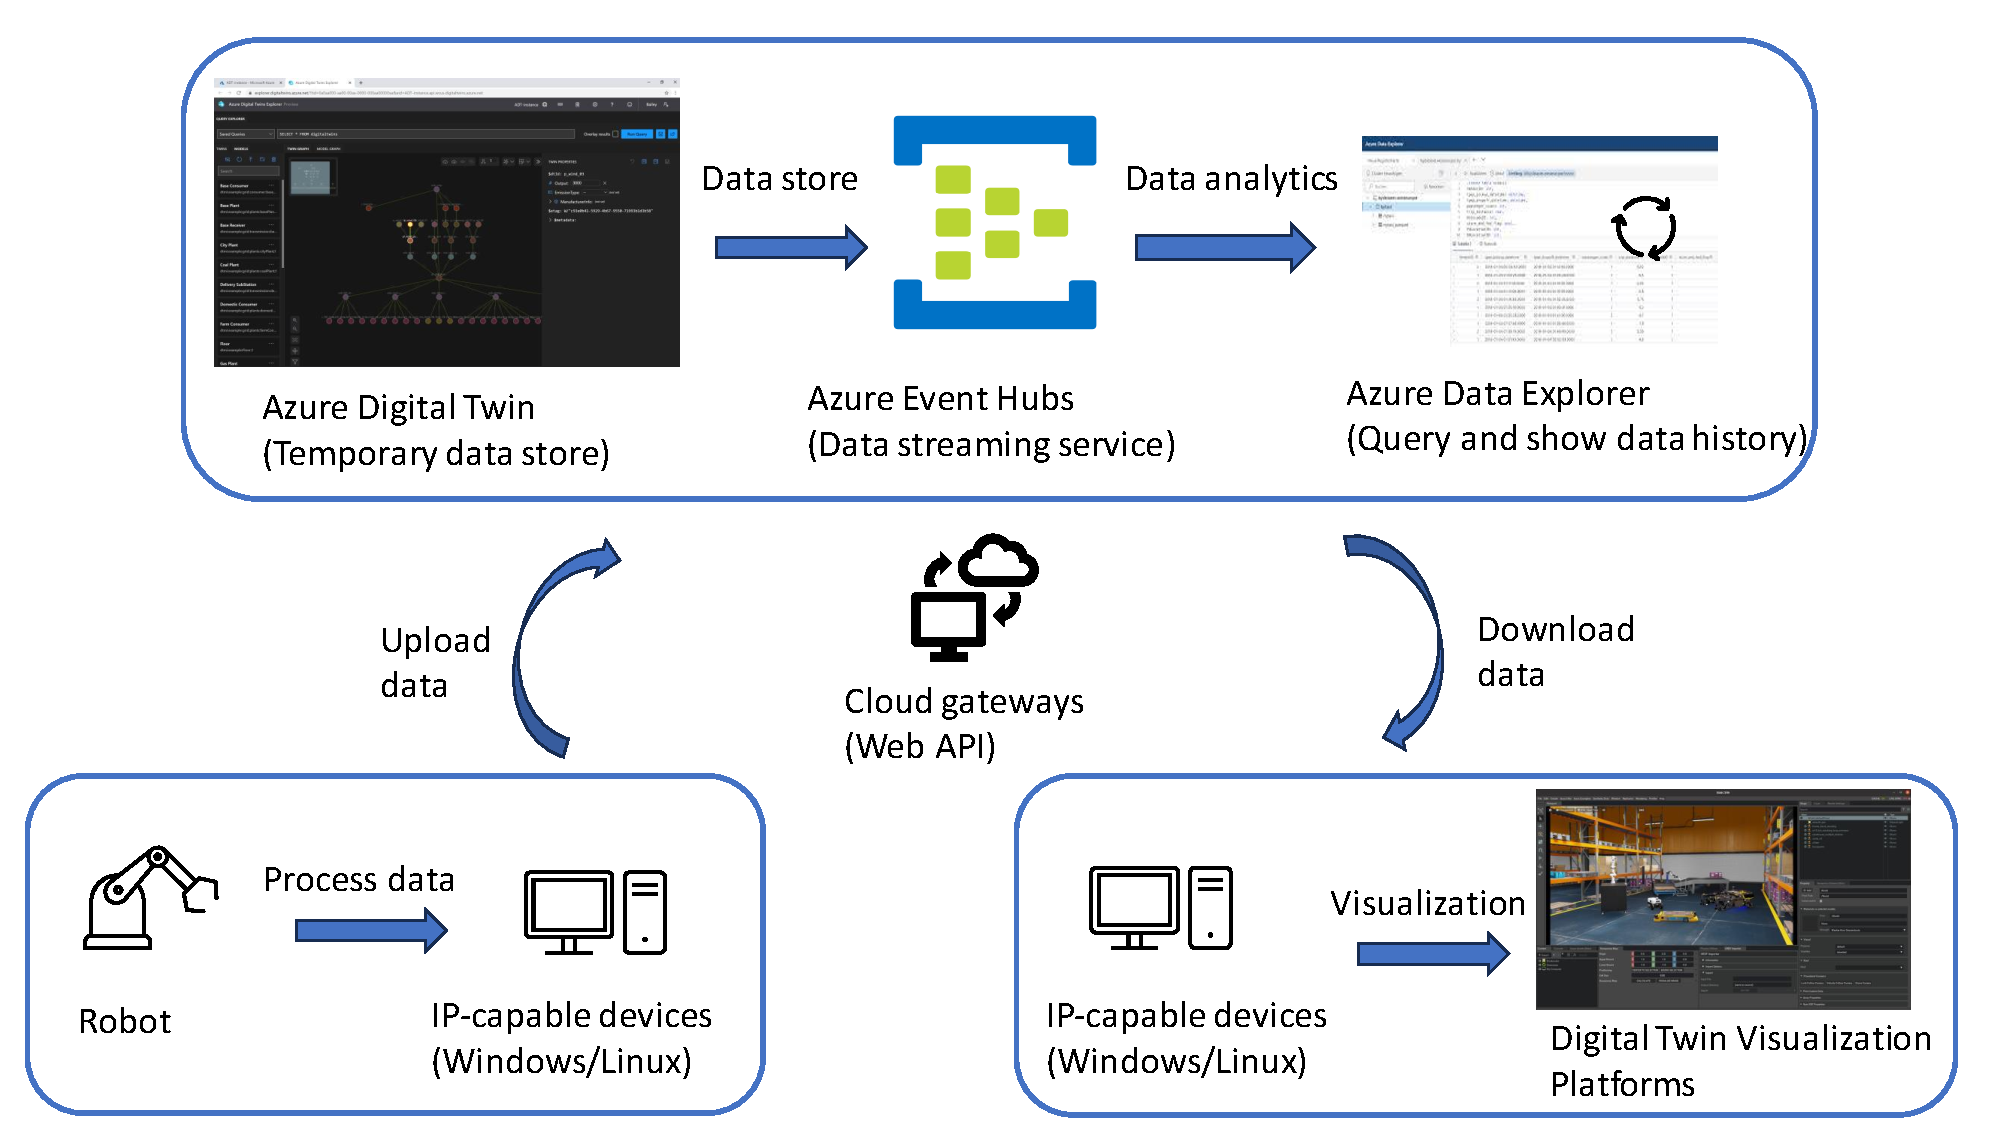
\includegraphics[width=\textwidth]{figures/DT_Conceptual_Diagram.pdf}

\centering
\caption{Conceptual diagram of MAS\label{fig: DTConceptual}}
\end{figure}

The workflow of updating global digital twin through the \gls{dta} process is shown 
in Figure \ref{fig: DTConceptual}. The process begins on the left-hand side of the 
graph, where the \gls{dta} receives process data from robots, including steady-state 
data. The process data is parsed and uploaded one by one to the Azure Digital Twins 
platform after separating the sticky packets from the \gls{tcp} socket.
All the updates of the digital twin instances in the cloud are temporarily displayed 
in Azure Digital Twins Explorer and concurrently stored in Azure Event Hubs. The history 
data can be ingested for further analysis in Azure Data Explorer. The Azure Digital Twins 
Explorer serves as a robot status monitor, while Azure Data Explorer is a data analysis tool.
Once the remote data update is successful, the data is immediately downloaded to the local 
host and can be used as input for other visualization purposes. The real-time capability 
of this upload and download cycle of data should also be maintained.

It is important to note that the process data is generated by robot movement, 
which means that the \gls{dta} is completely independent of the \gls{mas}. This decoupling 
offers a 
significant advantage. Even if the \gls{mas} is in complete chaos, the robot's current status 
will still be captured and updated remotely. This is advantageous for both data acquisition 
and monitoring purposes.



\subsection{Prerequisite} \label{chap: ntpsetup}
\subsubsection{\gls{ntp} setup}
In order to measure the delays between the local host and cloud, the clock of both ends must be synchronized. 
Due to the nature of computer systems, the software clock might drift away from the "true" time (absolute \gls{utc}) 
due to various reasons like system load, hardware imperfections, or even temperature changes.
Therefore, before the measurement, the software clock of the local host should be synchronized with the global 
clock using \gls{ntp}. 
The \gls{ntp} setup of the Linux system is as follows:  

\begin{enumerate}
    \item System update and upgrade.
    \item Install \gls{ntp}.
    \item Add reliable global \gls{ntp} servers/server pools to configure ntp.conf file.
    \item Allow port 123/udp for or disable firewall.
    \item Restart \gls{ntp} and check \gls{ntp} status.
    \item Check synchronization status (e.g.: reach, delay, offset and jitter, etc).
    \end{enumerate}

Since the cloud system clock is already synchronized with \gls{utc}, all the tests and calculations results are based on \gls{utc}. 

\subsection{Pseudo-Code of \gls{rcp} and \gls{dta} workflow in C++ and C\#}\label{chap: RCPDTAPseudo}

As previously mentioned in this chapter, it is important to completely separate the 
\gls{dta} from the \gls{mas}. Algorithms \ref{alg:RCPPseudoCode} and 
\ref{alg:DTAgentPseudoCode} list the workflows of \gls{rcp} and \gls{dta} separately. 
In the \gls{rcp} workflow, the robot arm is controlled through predefined functions 
that can record the current states. Each new state recorded must be immediately sent 
to the \gls{dta} via the established \gls{tcp} socket. 
On the \gls{dta} side, it must be started before the \gls{rcp} and listen to the 
socket to receive the data stream once connected. Whenever a new connection to a 
\gls{ra} is established, the \gls{dta} will create a new thread to receive, process, 
upload and download data concurrently. 
However, an issue with using \gls{tcp} is that packets do not arrive individually 
but are stuck together. To solve this, delimiters are utilized for sticky packet separation.

%pseudo code for RCP
\begin{breakablealgorithm}
    \caption{Pseudo-Code of \gls{rcp} workflow}
    \label{alg:RCPPseudoCode}
    \begin{algorithmic}
    \State {Import} socket, franka
    \State {Initialize} \gls{dta}\_IP
    \State \textbf{function} {$get\_rstate\_and\_send(clientSocket)$}
        \State \qquad Start robot motion and record robot state
        \State \qquad {$send\_message(robotState, clientSocket)$}
    \State \textbf{function} {$send\_message(msg, clientSocket)$}
        \State \qquad send robot state to \gls{dta} 
    \State \textbf{Main:}
    \State \qquad Instantiate robot
    \State \qquad Initialize start position
    \State \qquad Establish a \gls{tcp} connection with \gls{dta}  
    \State \qquad {$get\_rstate\_and\_send(clientSocket)$}
    \State \textbf{End}
    \end{algorithmic}
\end{breakablealgorithm}


%pseudo code for DTAgent
\begin{breakablealgorithm}
    \caption{Pseudo-Code of \gls{dta} workflow}
    \label{alg:DTAgentPseudoCode}
    \begin{algorithmic}
    \State {Import} socket, AzureDigitalTwin
    \State {Initialize} \gls{rcp}\_IP(s)
    \State \textbf{function} {$read\_and\_upload\_download\_processData(\gls{rcp}\_IP)$}
        \State \qquad \textbf{do run in parallel}
            \State \qquad \qquad $create\_client\_thread(\gls{rcp}\_IP)$       
    \State \textbf{function} {$create\_client\_thread(\gls{rcp}\_IP)$}
        \State \qquad Establish a \gls{tcp} connection with \gls{ra}
        \State \qquad {$data = read\_data(clientSocket)$}  
        \State \qquad {$process\_data\_upload\_and\_download(data)$}    
    \State \textbf{function} {$read\_data(clientSocket)$}
        \State \qquad receive and store robot state data
        \State \qquad \textbf{return} data
    \State \textbf{function} {$process\_data\_upload\_and\_download(data)$}
        \State \qquad separate sticky packets with delimiter
        \State \qquad upload processed data to Azure Digital Twins in json patch
        \State \qquad download twin after data update 
    \State \textbf{Main:}
        \State \qquad \textbf{for} \gls{rcp}\_IP in IPs \textbf{do}
        \State \qquad \qquad {$read\_and\_upload\_download\_processData(\gls{rcp}\_IP)$}
        \State \textbf{End}
    \end{algorithmic}
\end{breakablealgorithm}



\subsection{Azure Digital Twins}
According to the workflow explained in section \ref{chap: Overview-External}, 
it is crucial to establish a reliable and operational Azure Digital Twins platform 
to ensure seamless data transfer. The platform should include Azure Digital Twins Explorer, 
Azure Event Hub, and Azure Data Explorer. Additionally, the Azure Digital Twins 
instance must be configured with a time-series data history connection. Other resources 
must also be created, such as an Event Hubs namespace, an event hub, Azure Data Explorer 
cluster, and a database. 
After a connection, data is sent to an event hub, which eventually forwards the data to 
the Azure Data Explorer cluster and stores it in a database. The history data includes 
twin property updates, twin lifecycle events, and relationship lifecycle events, which 
can be later queried in Azure Data Explorer.

\subsubsection{Setup}
Here is the sequence of the basic setup in the Azure platform:
\begin{enumerate}
    \item Create Azure Event Hub namespace and add instance.
    \item Create Azure Data Explorer cluster and add database.
    \item Connect data history of the Event Hub instance to the digital twin instance.
\end{enumerate}

In order to verify whether the connection is successful, one can try updating the 
digital twin instance and querying data from the Azure Data Explorer side. The query
language is called \gls{kql}, which is powerful for pattern discovery, anomalies 
and outliers identification, and statistical modeling (various graphs creation). 
Following algorithm \ref{alg: KQLCode} is a snippet of the example \gls{kql} code in the test: 

\begin{algorithm}
    \caption{\gls{kql}}
    \label{alg: KQLCode}
    \begin{algorithmic}
        \State  AdtPropertyEvents 
        \State {| where ID == 'RadPositionJoint3' and Key == 'value'}
        \State {| where TimeStamp between (datetime(2023-08-27 16:02) .. datetime(2023-08-27 19:00))}
        \State {| order by TimeStamp asc}
        \State {| project TimeStamp, Id, Key, Value}
    \end{algorithmic}
\end{algorithm}


\begin{figure}[htb]
    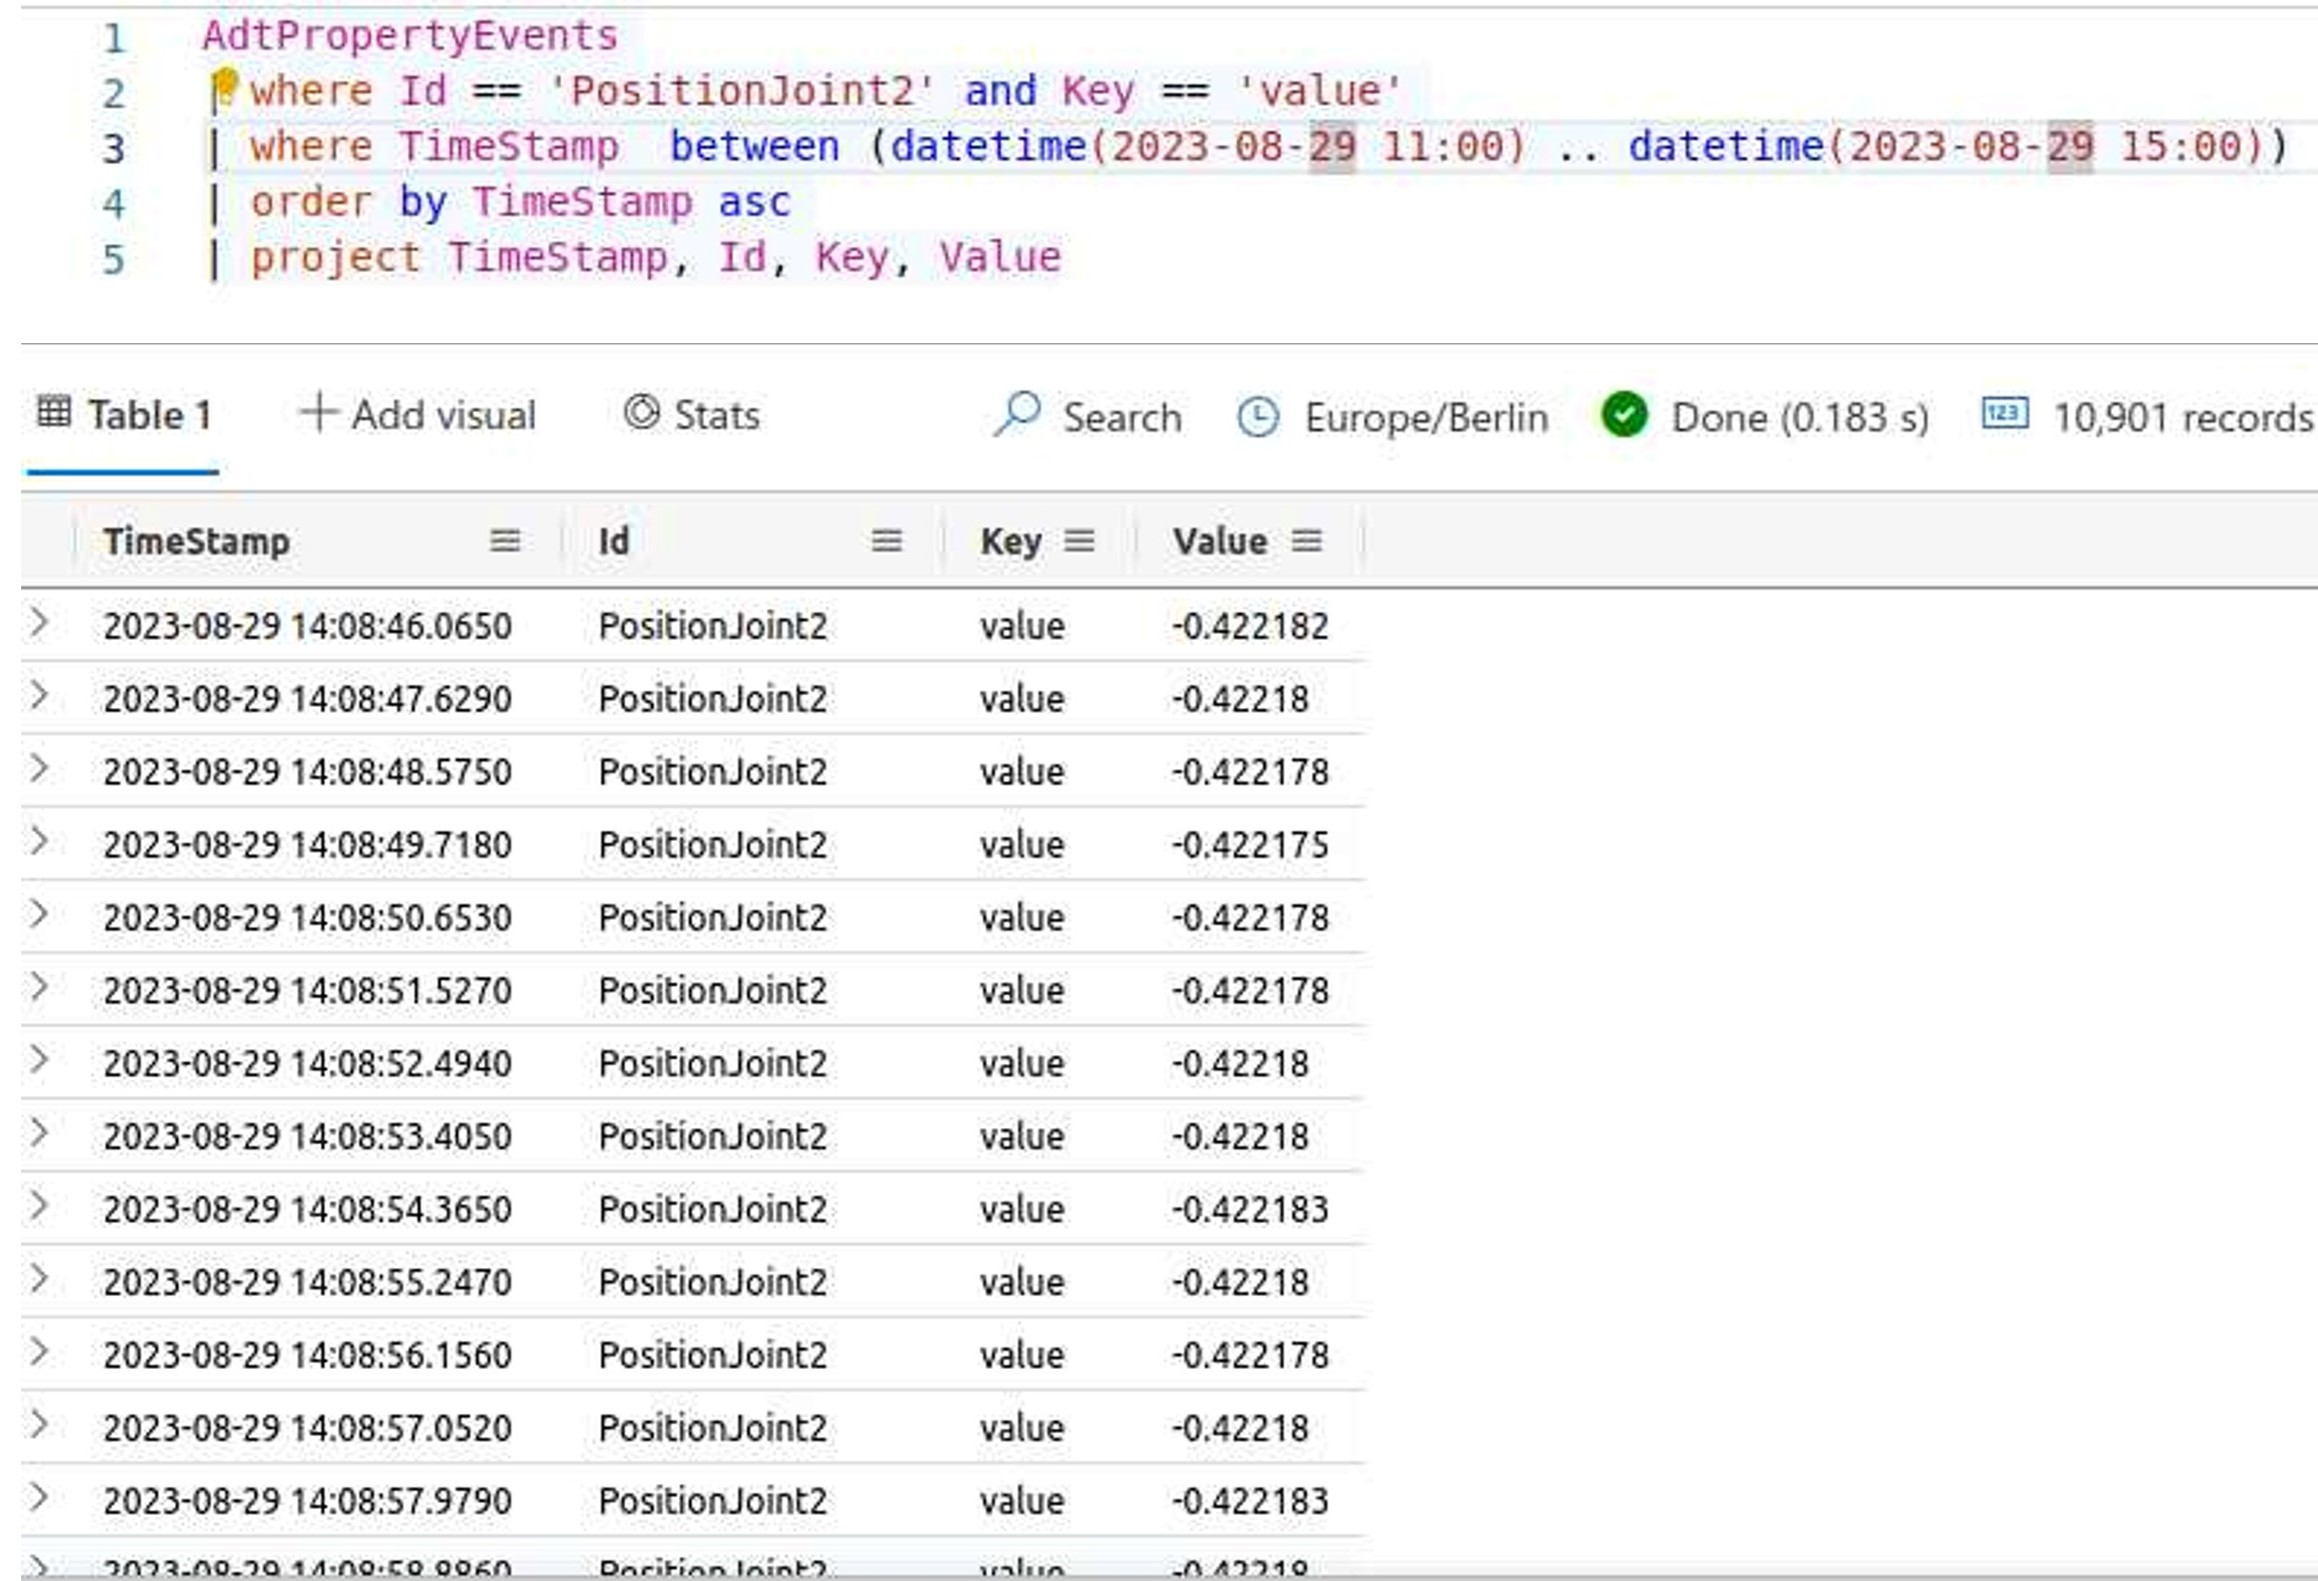
\includegraphics[width=\textwidth]{figures/KQL_cut.jpg}
    
    \centering
    \caption{Snippet of Data Explorer\label{fig: KQL}}
\end{figure}

As shown in fig.\ref{fig: KQL}, by executing the code from the snippet, all the history data will be listed as a table 
which can be downloaded to the local devices later. 


\section{Modularization}\label{chap: Meth-Modular}
In addition to the internal and external designs of a general \gls{mas}, 
there are also some considerations of modularizing timing behaviors of the 
system. In the following sections, the \gls{tcp/ip} model as well as 
\gls{dsl} will be introduced and used as the design basis of a modularized general 
\gls{mas}. 
\subsection{From \gls{osi} model to \gls{tcp/ip} model}

Although TCP is classified as a transport layer protocol according to the 
OSI model (fig.\ref{fig: OSI}), data transport between different TCP sockets 
still involves all layers. This is because a program using socket libraries 
operates the TCP socket, which is an operation under the application layer. 
The transport layer protocols only accept data from the session layer in the 
OSI model and break it down into smaller pieces to ensure reliable and correct 
data transport. However, considering delays in all seven layers for modularization 
purposes would be too strict and complicated. Therefore, the focus should be 
shifted from the general OSI model to the more abstract TCP/IP model, as depicted 
in fig.\ref{fig: TCP_IP}.

The TCP/IP model consists of four layers: application layer, transport layer, 
internet layer, and network access layer, with each mapping different layers in 
the OSI model. As depicted in the TCP/IP model, the application layer roughly 
contains the upper three layers, while the network access layer contains the 
physical and data link layer. The network layer is renamed as the internet 
layer, while the transport layer remains the same.

\begin{figure}[htb]
    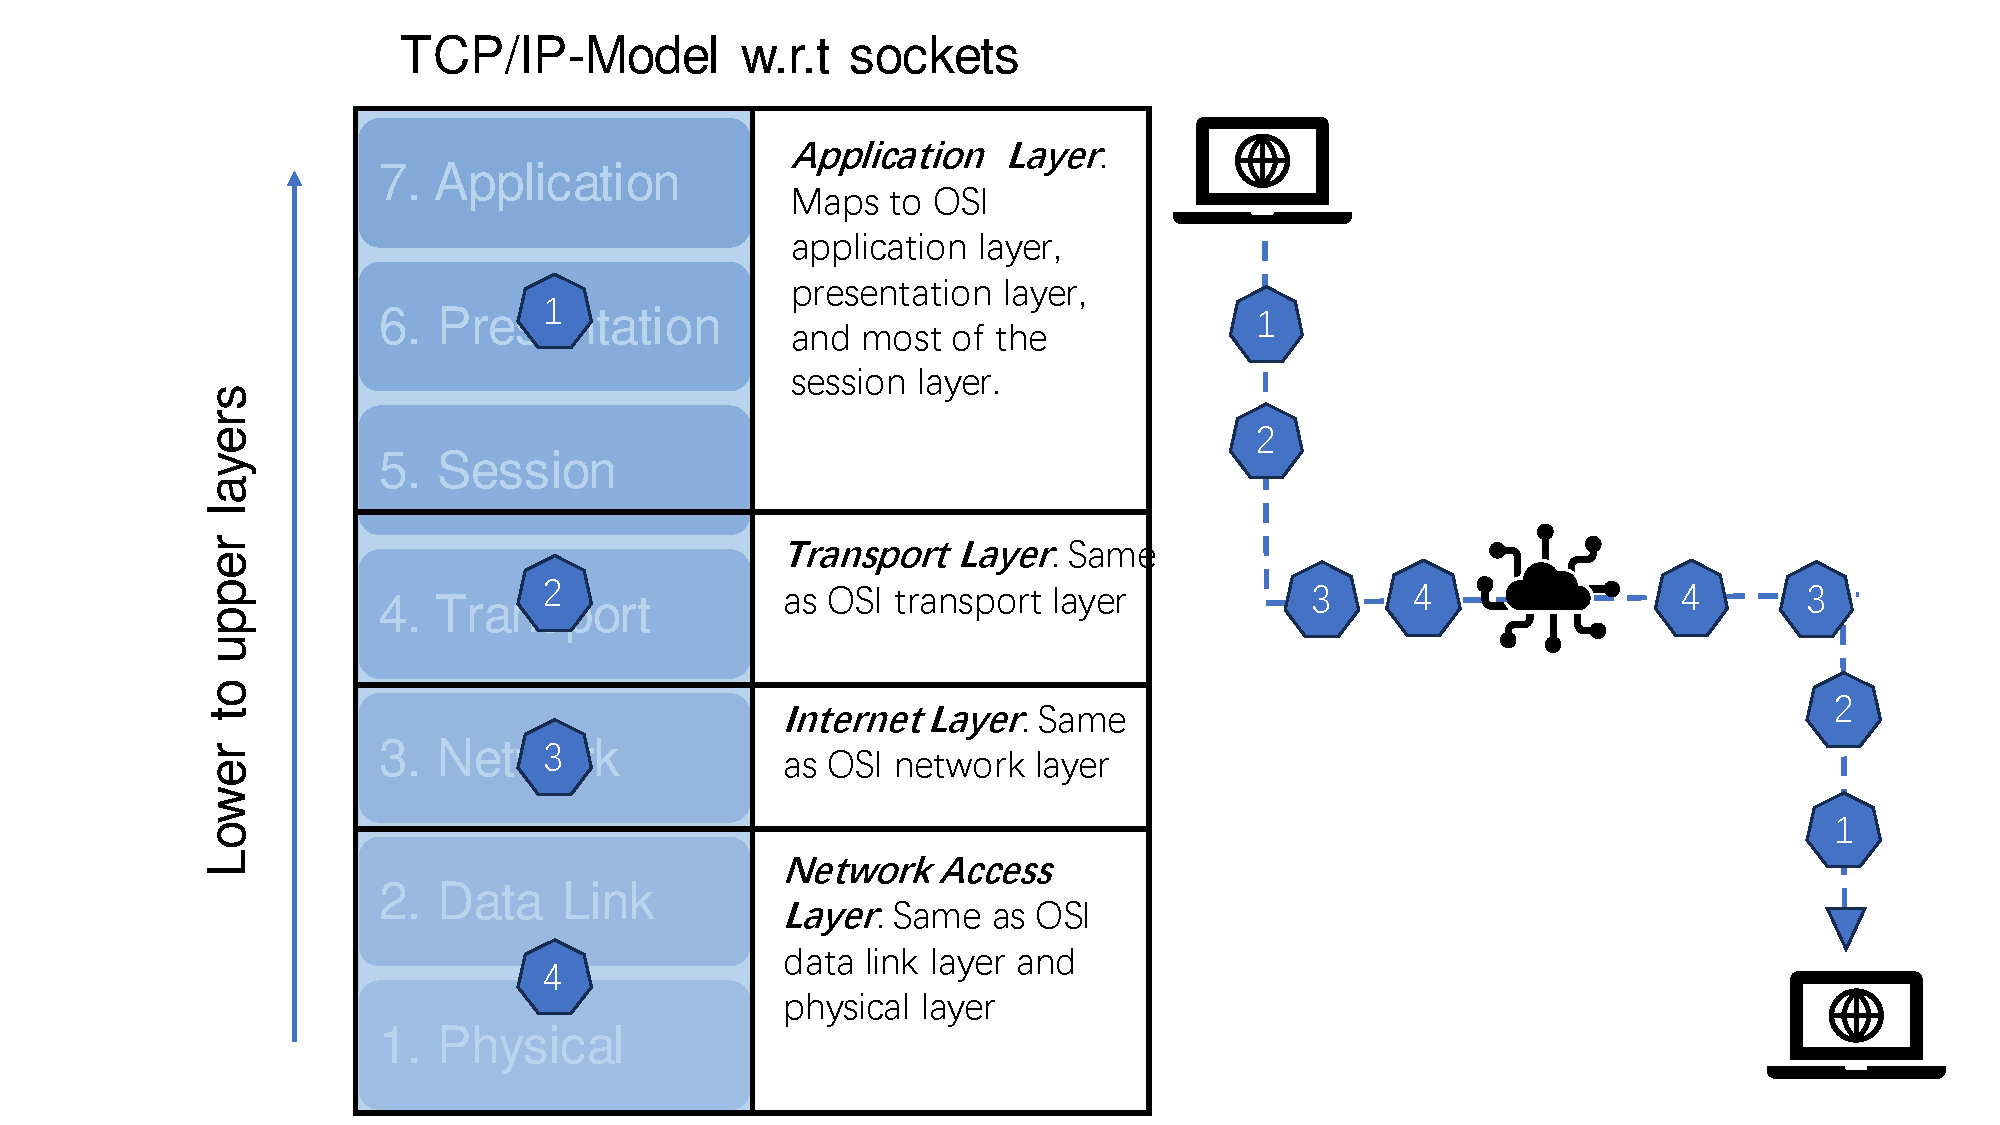
\includegraphics[width=\textwidth]{figures/TCP_IP.pdf}
    
    \centering
    \caption{\gls{tcp/ip} model with example protocols \label{fig: TCP_IP}}
\end{figure}

\subsection{Timing properties of data transport w.r.t sockets and visual notations based on \gls{tcp/ip} model}
When operating in an application, both TCP sockets and WebSockets transport packets 
through all layers of the TCP/IP model. In order to better modularize delay, a set of 
visual notations based on \gls{dsl} is created.
Thanks to the works of former researchers, there are already some graphical tools 
developed for different purposes. The graphical tools 
can be roughly divided into two types: tools ideal for real-world delay measurement, 
for example, the famous Wireshark, OPNET, and NS-3, 
and tools suitable for modeling and visualization, such as OpenModelica, 
Matlab/Simulink and LabVIEW.



Although being out of the scope of this thesis, the measurement of delay within 
each layer of \gls{tcp/ip} model will be essential for future investment.
For instance, as depicted in figure \ref{fig: DSLConceptual}, the delay in 
each layer is represented as a block based on \gls{dsl}, which can be later integrated 
with graphical tools.
In this case, delay in a specific network layer will become comparable between different 
technologies based on either application or transport layer protocols, for example, 
\gls{tcp} socket and WebSocket. Apart from the network delay of communication between 
agents, as shown in the figure, there is also another delay that can be modularized in 
the context of robot control. The robot control systems introduce delay first in \gls{rci} 
by executing the commands and then a minor delay within the I/O module before activating 
the actuator.
After each robot motion driven by the actuator, its current state will be sent back to 
the \gls{cpu} by first going through the sensor, I/O module, and \gls{rci} again. 







\begin{figure}[htb]
    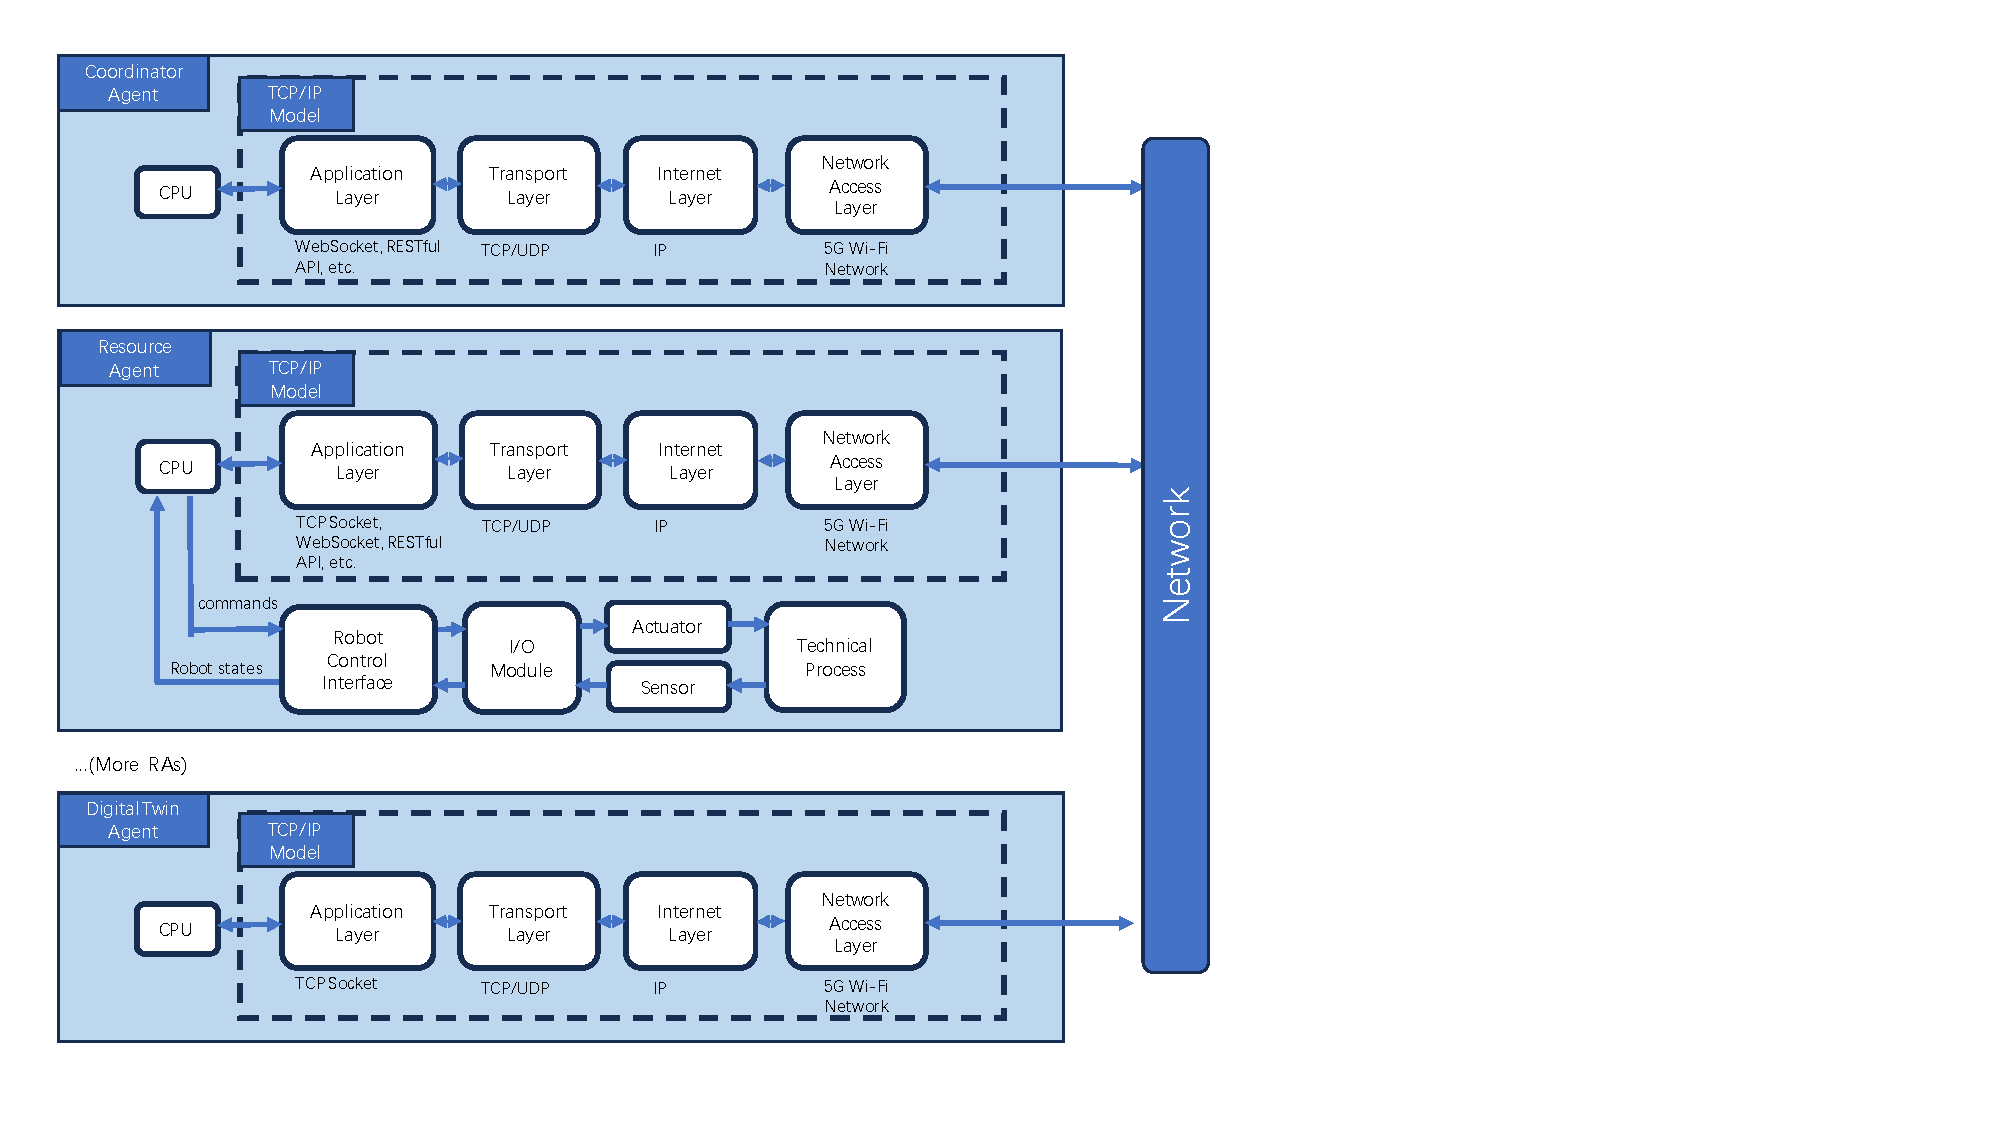
\includegraphics[width=\textwidth]{figures/DSLConceptual.pdf}
    
    \centering
    \caption{Conceptual diagram of a modularized general \gls{mas} based on \gls{dsl} \label{fig: DSLConceptual}}
\end{figure}
%
\chapter{Implementation and discussion} \label{chap: Result}

In order to verify the feasibility of the methodologies from chapter \ref{chap: Meth}, 
performance testing based on assumptions and two industrial uses cases 
are done and their results will be performed and discussed in this chapter. 
Again, the tests will also be divided into internal (\ref{chap: Result-Internal}) 
and external (\ref{chap: Result-External}) part, referring to those in chapter \ref{chap: Meth}.

\section{Internal}\label{chap: Result-Internal}
For the internal \gls{mas}, multiple tests are performed on the agent 
communication system. That means, the messages 
will be passed through the \gls{ca} under WebSocket architecture. 
Various tests will be done and the test results will be discussed later in section 
\ref{chap: Result-WS}. 
In addition to the performance testing of WebSocket architecture alone, 
a comparison between WebSocket and \gls{http} will be done to verify the feasibility 
of WebSocket. 
After that, tests relevant to packets prioritization will be performed in 
section \ref{chap: Result-priority}. 
Finally, tests results of the WebSocket based \gls{mas} architecture under 
BMW use case will be presented to close the sections.


\subsection{Test results of WebSocket in various performance testing including worst case scenarios} \label{chap: Result-WS}

After the construction a \gls{mas} under WebSocket, the speed, robustness, 
reliability and application size of the system will be examined by 
performance tests. 

\subsubsection{Increasing client numbers}
In real world, the number of clients will greatly influence the performance of 
server. Assume that all agents serve as clients and \gls{ca} as a central server. 
  

By handling an increasing number of connection requests, and the growing demands 
of data processing capacity, the average total delay with or without process time can be 
roughly described as an overall increasing pattern. However, it does not necessarily 
need to be linear based on several reasons. In exercise, concurrent programming 
will speed up the processing for a large computation problem. As depicted in 
fig.\ref{fig: proportional-clients}, the average process time from one to ten 
clients is decreasing with a better utilization of the CPU power due to 
concurrent processing. However, by further increasing the clients number, the 
speedup will be limited by CPU cores number. Assume that a CPU has 8 core, 
and each core can handle 2 threads, it will have in total 16 threads to perform tasks.
In WebSocket based \gls{mas} program, the asynchronous I/O framework asyncio is used 
to handle the coroutines execution in order to better utilize the threads power.
Therefore, the asyncio is potentially more suitable for larger computational tasks 
compared to synchronous single thread programming.

Obviously there is a limit of the clients number to prevent system breakdown. 
With one server handling all clients at once, there is a system timeout problem of 
the server when the clients number reaches 1000. Therefore, 
distributing clients with more servers becomes a possible solution. 


\begin{figure}[htb]
    \begin{subfigure}[b]{0.49\textwidth}
        \centering
        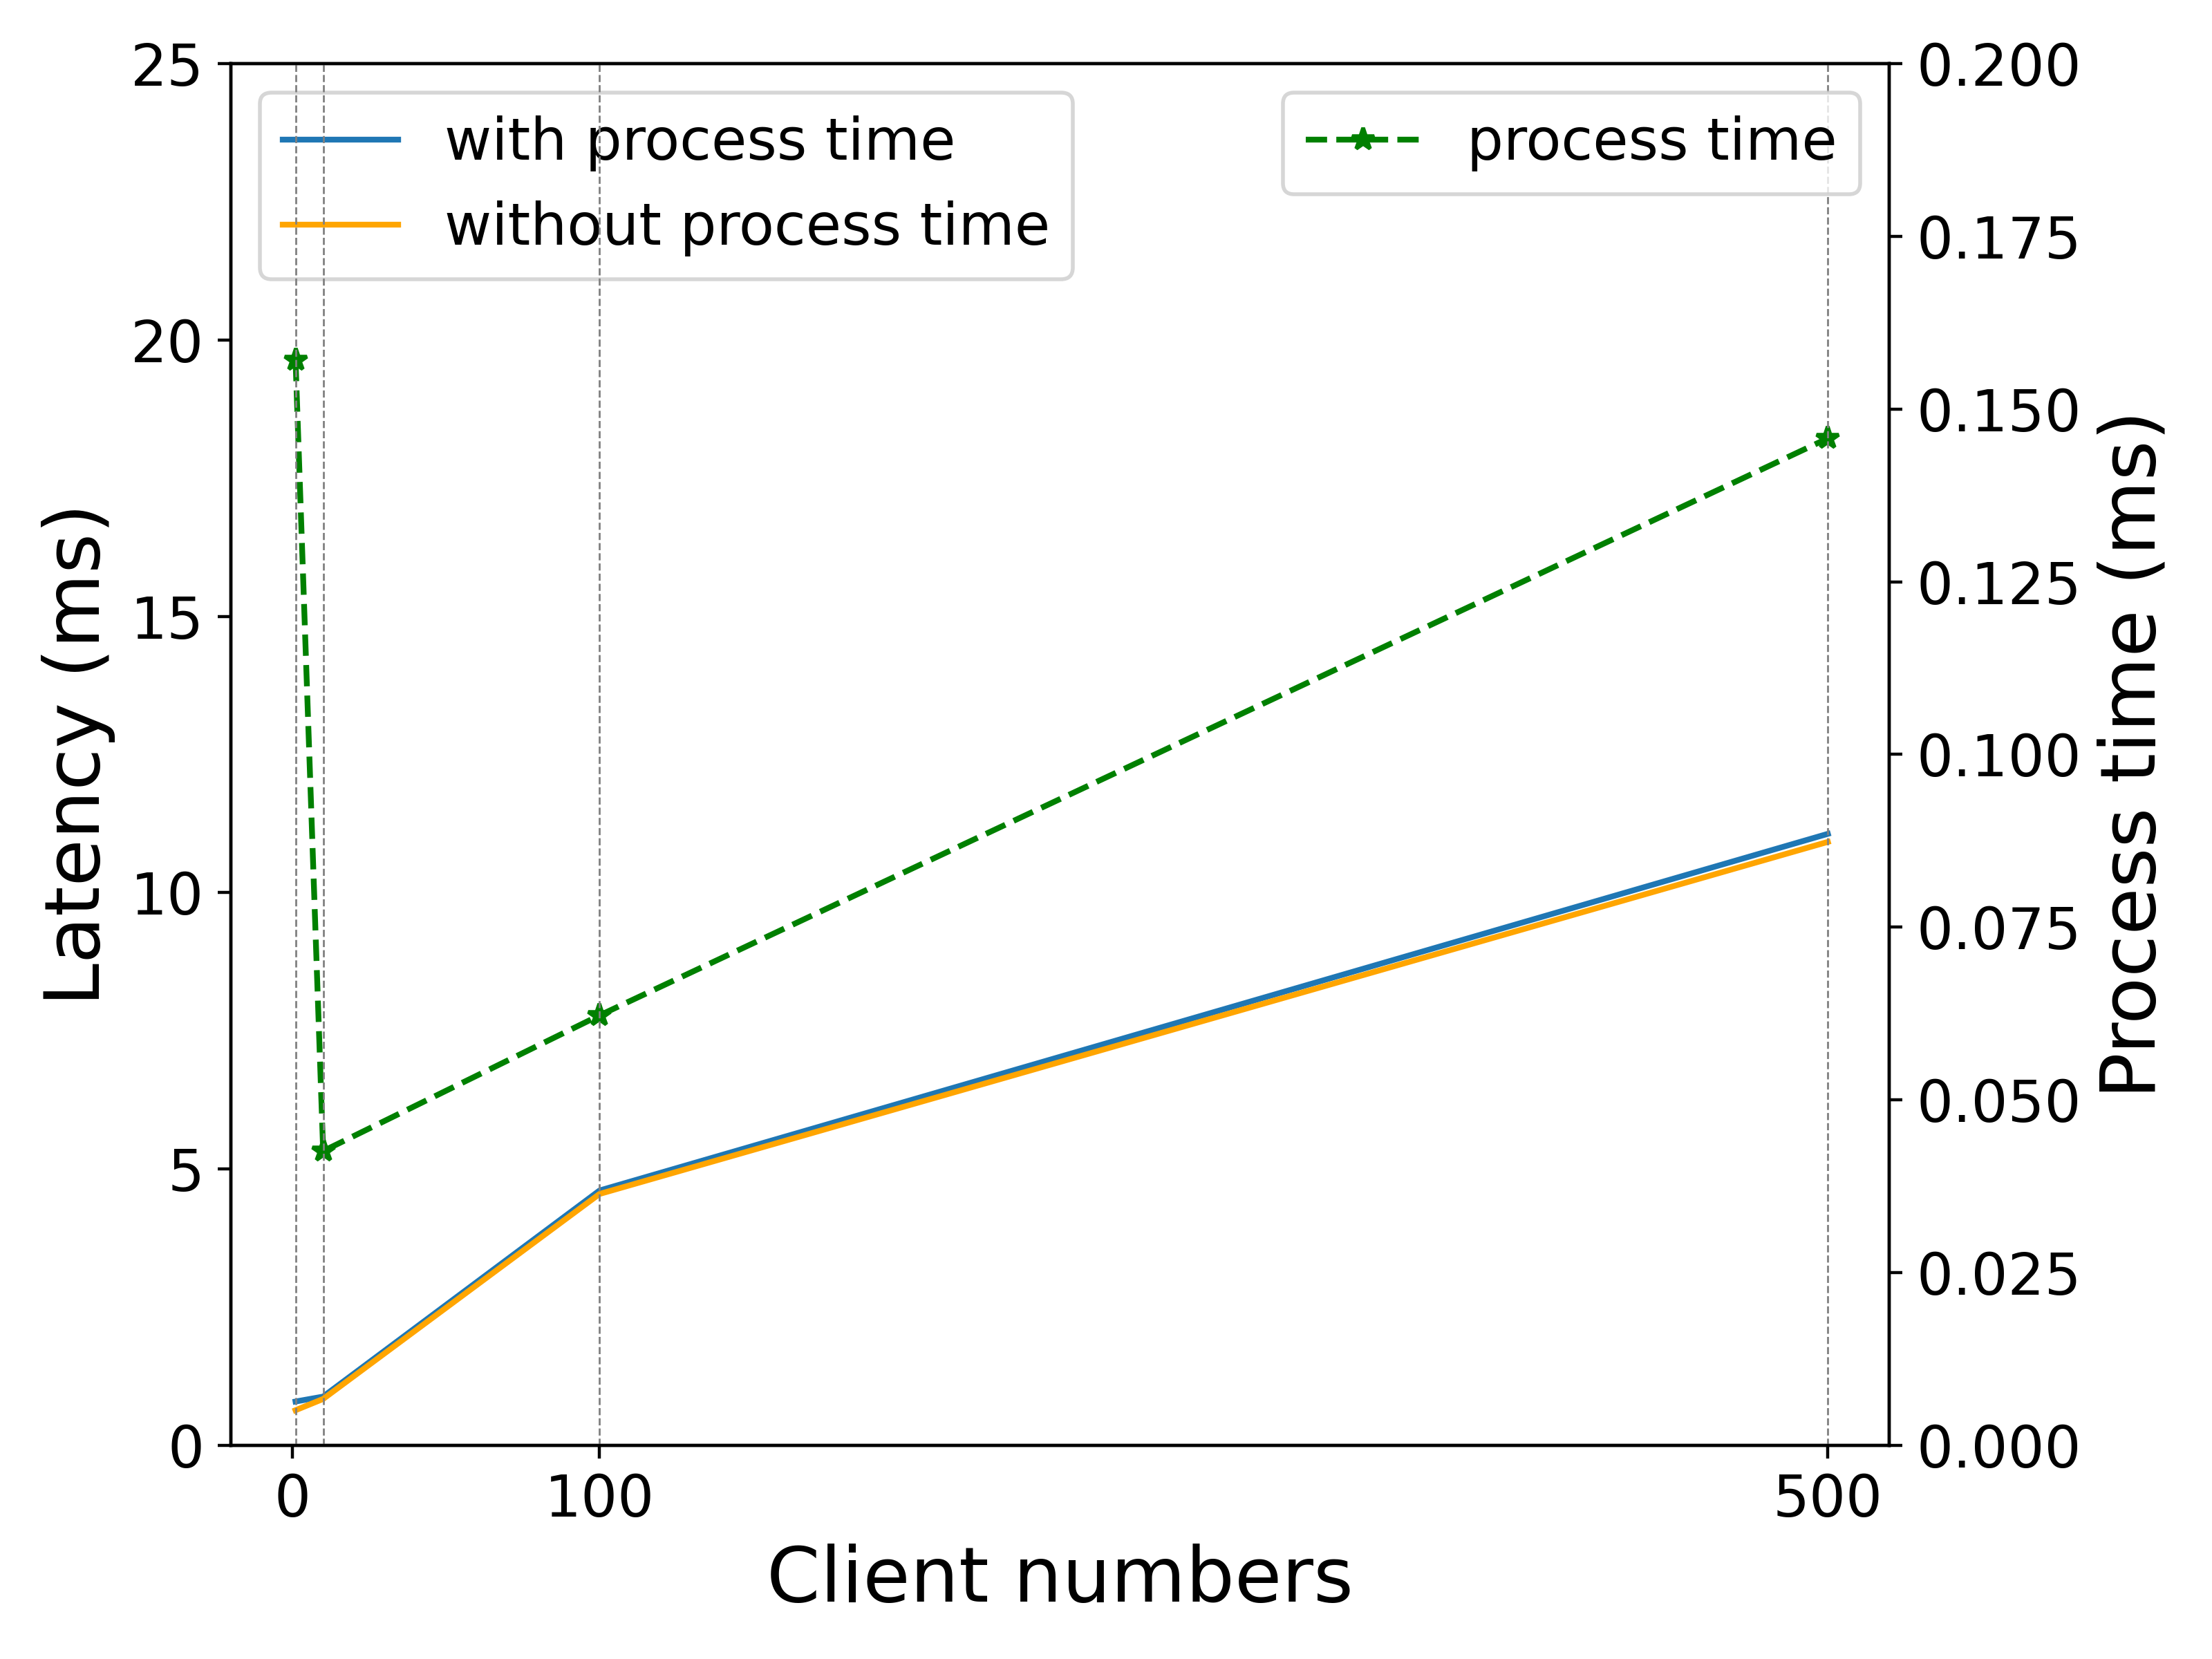
\includegraphics[width=\textwidth]{figures/tests/proportional_tests/Average_string_messages_sending_time_of_100_tests_of_diff_client_numbers.png}\hfill 
        \caption{} \label{fig: proportional-clients-a}
    \end{subfigure}
    \begin{subfigure}[b]{0.49\textwidth}
        \centering
        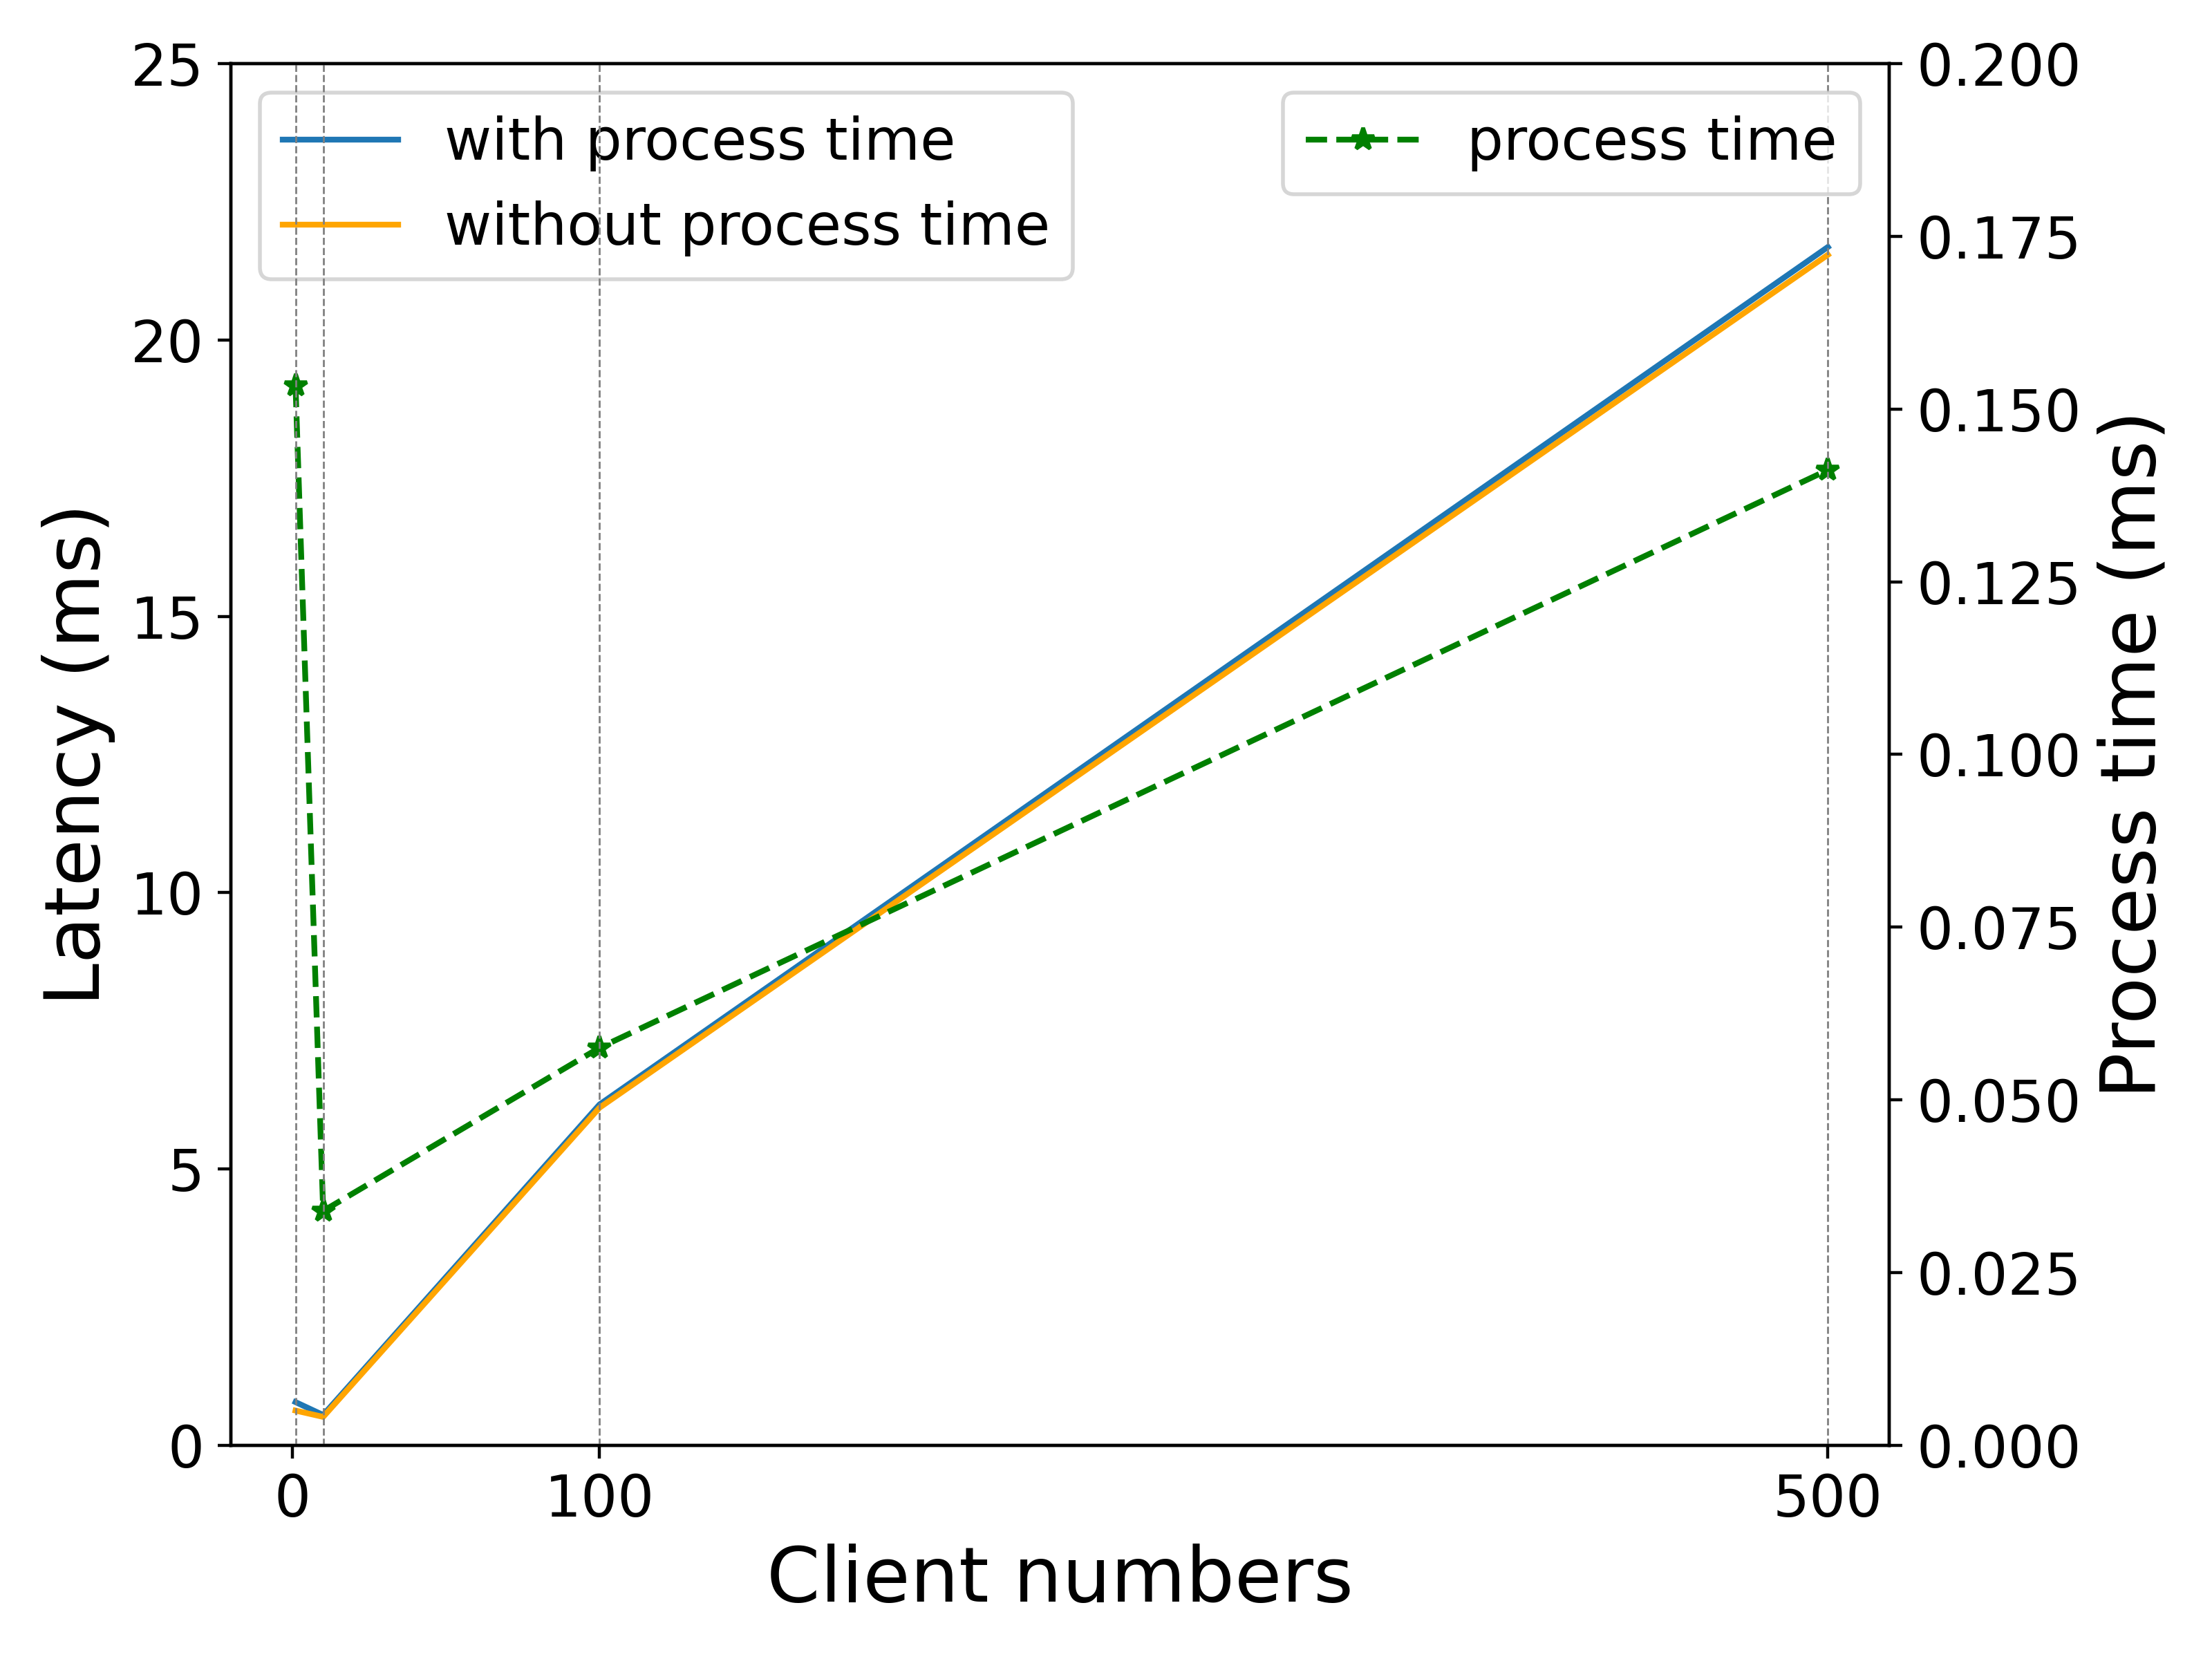
\includegraphics[width=\textwidth]{figures/tests/proportional_tests/Average_string_messages_receiving_time_of_100_tests_of_diff_client_numbers.png}\hfill 
        \caption{} \label{fig: proportional-clients-b}
        \end{subfigure}

    \caption{Average delay of sending a string message 100 times 
    to a clientR from 1, 10, 100 or 500 clients separately. (a) Messages sent forward, 
    and (b) response messages from clientR. 
    \label{fig: proportional-clients}}
\end{figure}


\subsubsection{Increasing server numbers}
Under the same condition where 1000 clients are sending and receiving messages from 
a clientR, the messages will be separated this time to two or three groups, with 
each passing through different servers. Limited by the hardware configuration 
for the external routing solutions according to fig.\ref{fig: NSConceptual}, only 
maximal three servers can be used for the test. However, several assumptions 
can be made based on the results from fig.\ref{fig: proportional-servers}. 


\begin{figure}[htb]
    \centering
    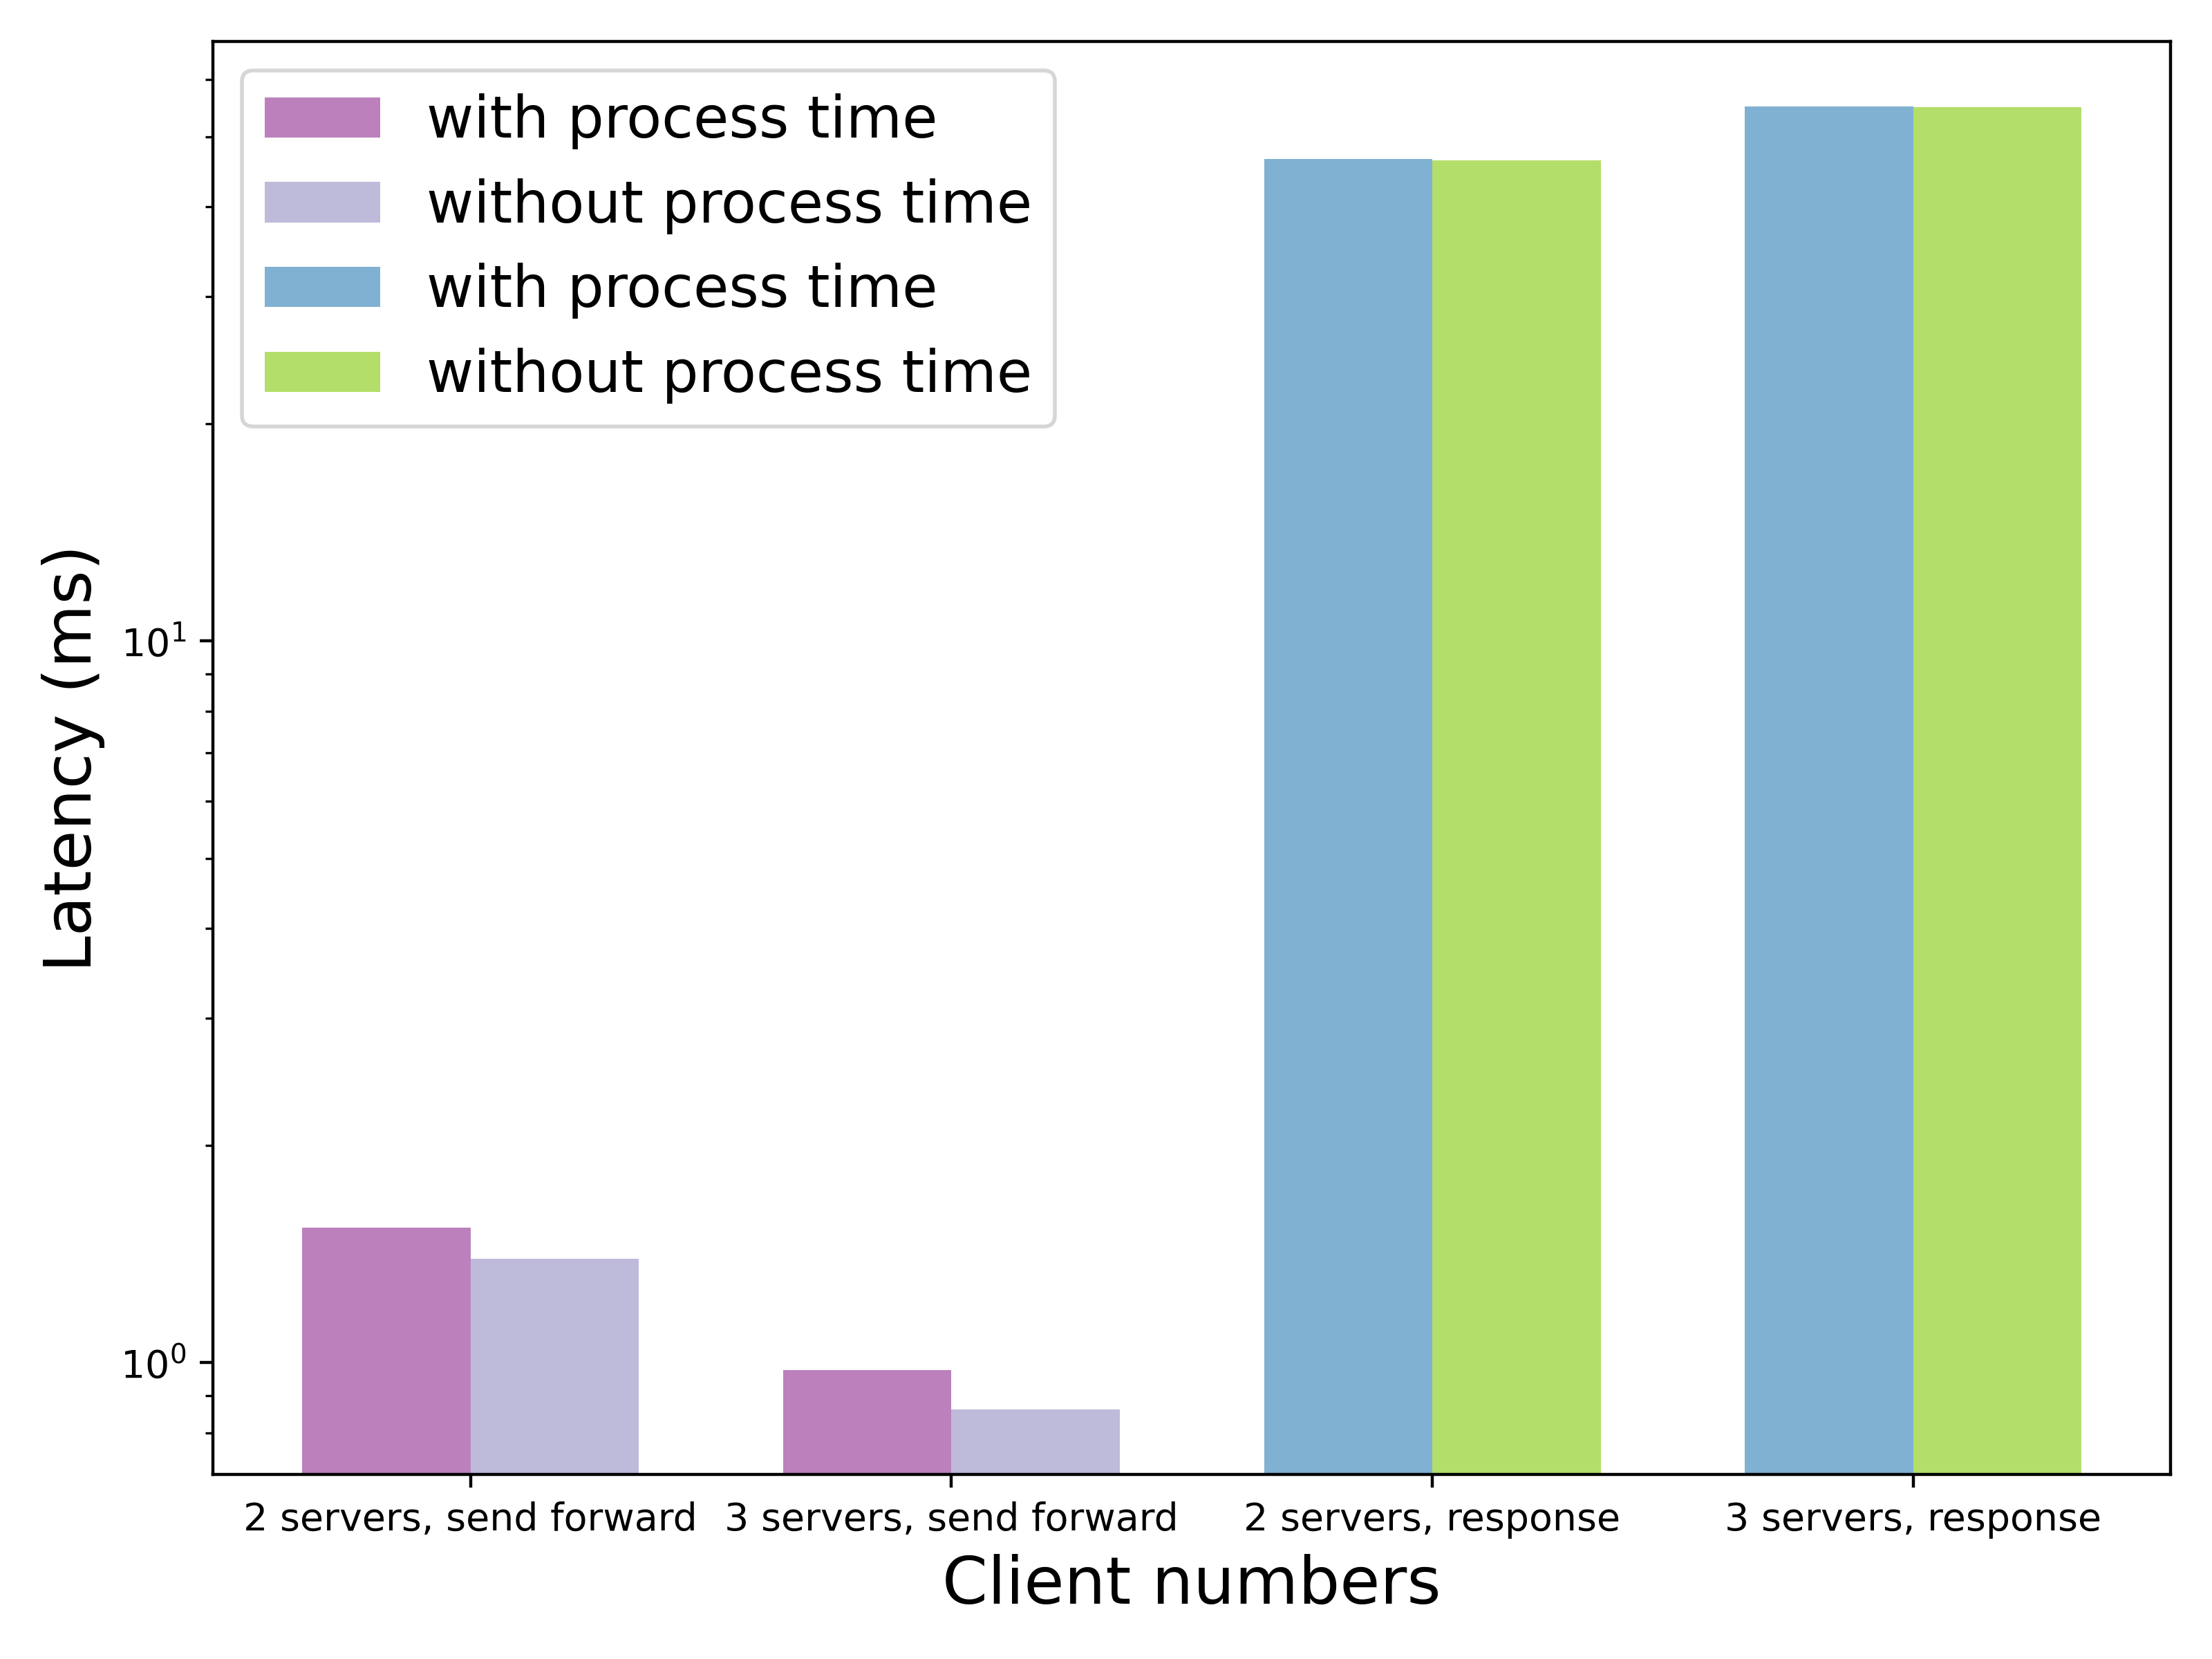
\includegraphics[width=0.8\textwidth]{figures/tests/proportional_tests/Average_string_messages_receiving_time_of_100_tests_diff_server_numbers.png}\hfill 
    \caption{Average delay of sending a string message 100 times 
    to a clientR from 1000 clients through 2 or 3 servers separately. 
    \label{fig: proportional-servers}}
\end{figure}

The latency reduction with an additional server according to 
fig.\ref{fig: proportional-servers} proves that, by introducing more servers 
to the system, the limited productive resources should be better utilized 
for frequent clients interactions. However, not as expected, the latency of 
response messages from clientR is much larger in fig.\ref{fig: proportional-servers},
which may also result from the CPU consumption. Since the send and receive 
processes in websocket are operated separately, and because of the high 
occupation of the CPU power when more than one server are running in the same 
device, the loads between each process might be unbalanced and added up by the 
increment of servers. 


\subsubsection{Increasing string message length}\label{chap: Result-Internal-string}
Another important test should be done to verify the influence of packet size (i.e., 
message length) to the system performance, according to the formula of packet 
transmission time: 
\begin{equation}
    Transmission $ $ delay = Packet $ $ size/Bandwidth
\end{equation}

If the bandwidth is determined, the transmission time with an increasing packet 
size should be linear. In the fig.\ref{fig: proportional-stringsize}, comparisons 
between different string message lengths varied from 1KB to 10MB are examined. 
The linear dependency of latency and string size in both forward 
(fig.\ref{fig: proportional-stringsize-a}) and return message (fig.\ref{fig: proportional-stringsize-b}) 
has verified the transmission time formula. It is also noticeable that the server 
process time increases by the rising message byte number. In real world scenarios, 
a large string message should be chunked into smaller pieces for communication, 
which will significantly reduce the process time consumption. For the purpose of system limit 
inspection, a string with the size up to 100MB is also tested and resulting in 
system timeout error, which already exceeds the server maximal 
processing capacity. 


\begin{figure}[htb]
    \begin{subfigure}{0.49\textwidth}
        \centering
        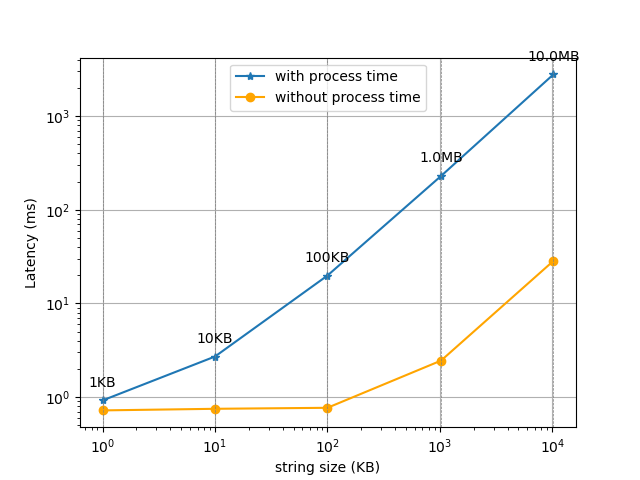
\includegraphics[width=\textwidth]{figures/tests/proportional_tests/log_Average_string_messages_sending_time_of_100_tests_1KB_to_10MB.png}
        \caption{} \label{fig: proportional-stringsize-c}
    \end{subfigure}
    \begin{subfigure}{0.49\textwidth}
        \centering
        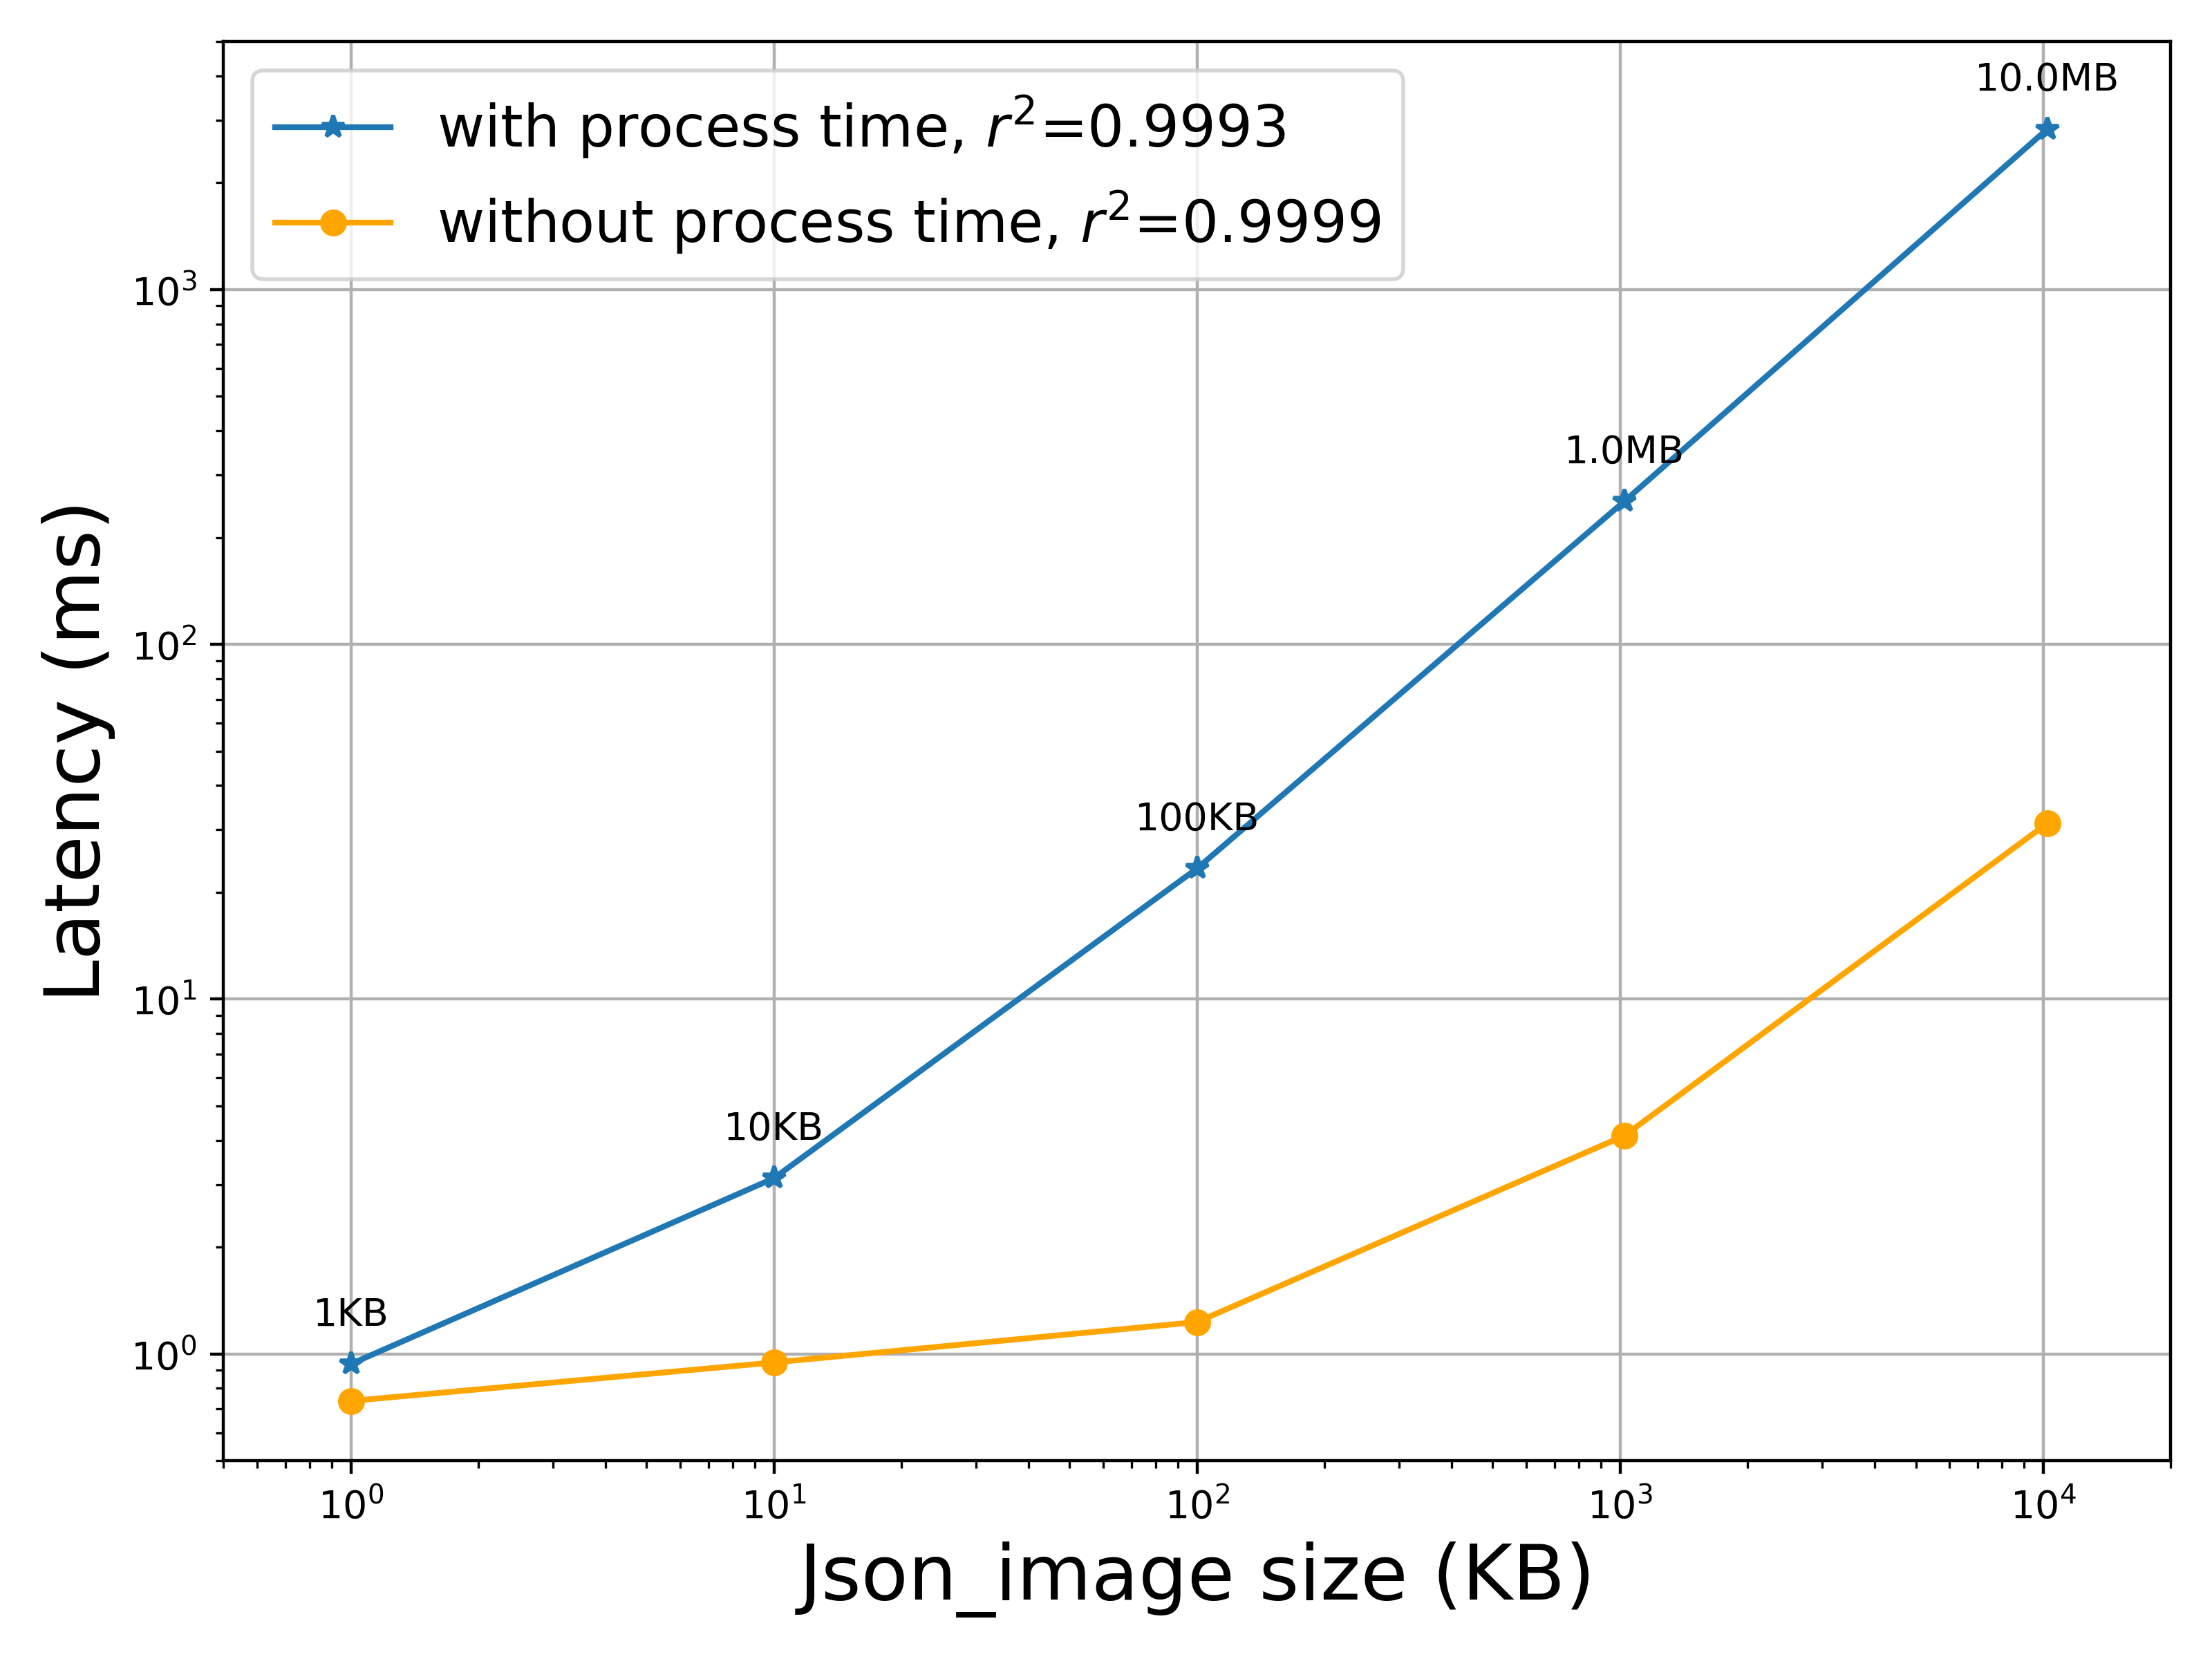
\includegraphics[width=\textwidth]{figures/tests/proportional_tests/log_Average_string_messages_receiving_time_of_100_tests_1KB_to_10MB.png}
        \caption{} \label{fig: proportional-stringsize-d}
    \end{subfigure}

    \begin{subfigure}{0.49\textwidth}
        \centering
        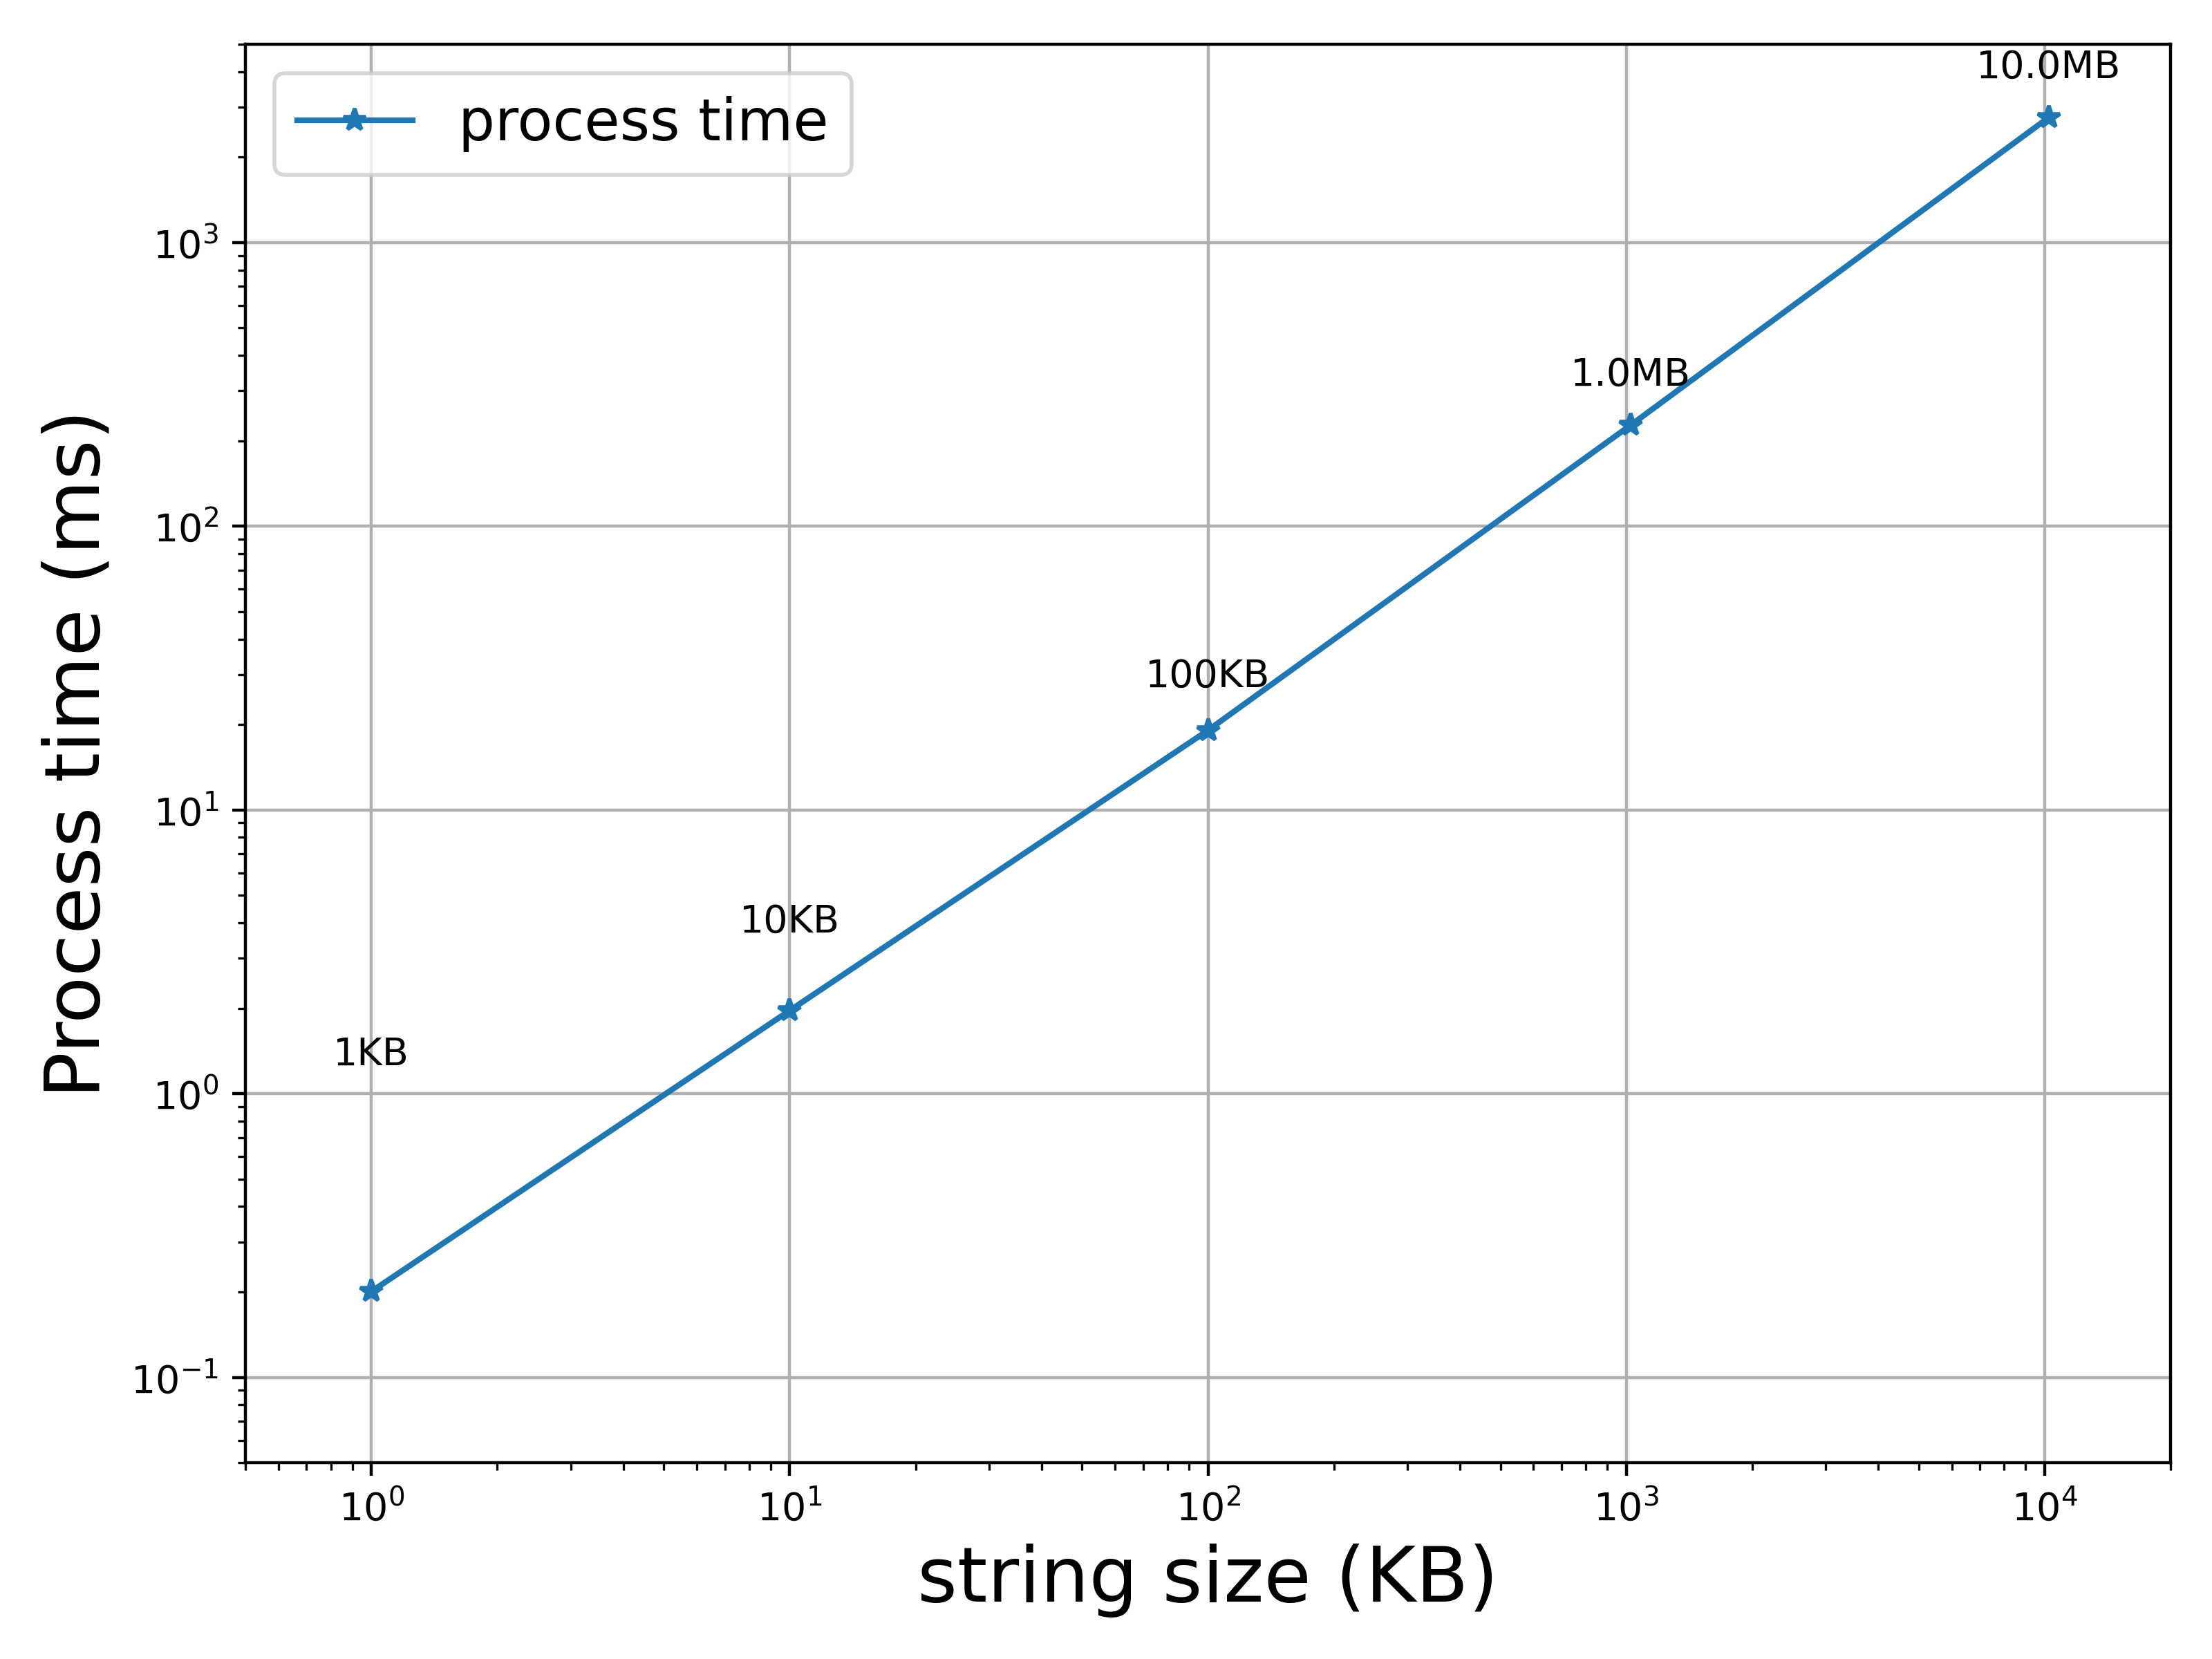
\includegraphics[width=\textwidth]{figures/tests/proportional_tests/Average_string_messages_sending_time_of_100_tests_1KB_to_10MB.png}
        \caption{} \label{fig: proportional-stringsize-a}
    \end{subfigure}
    \begin{subfigure}{0.49\textwidth}
        \centering
        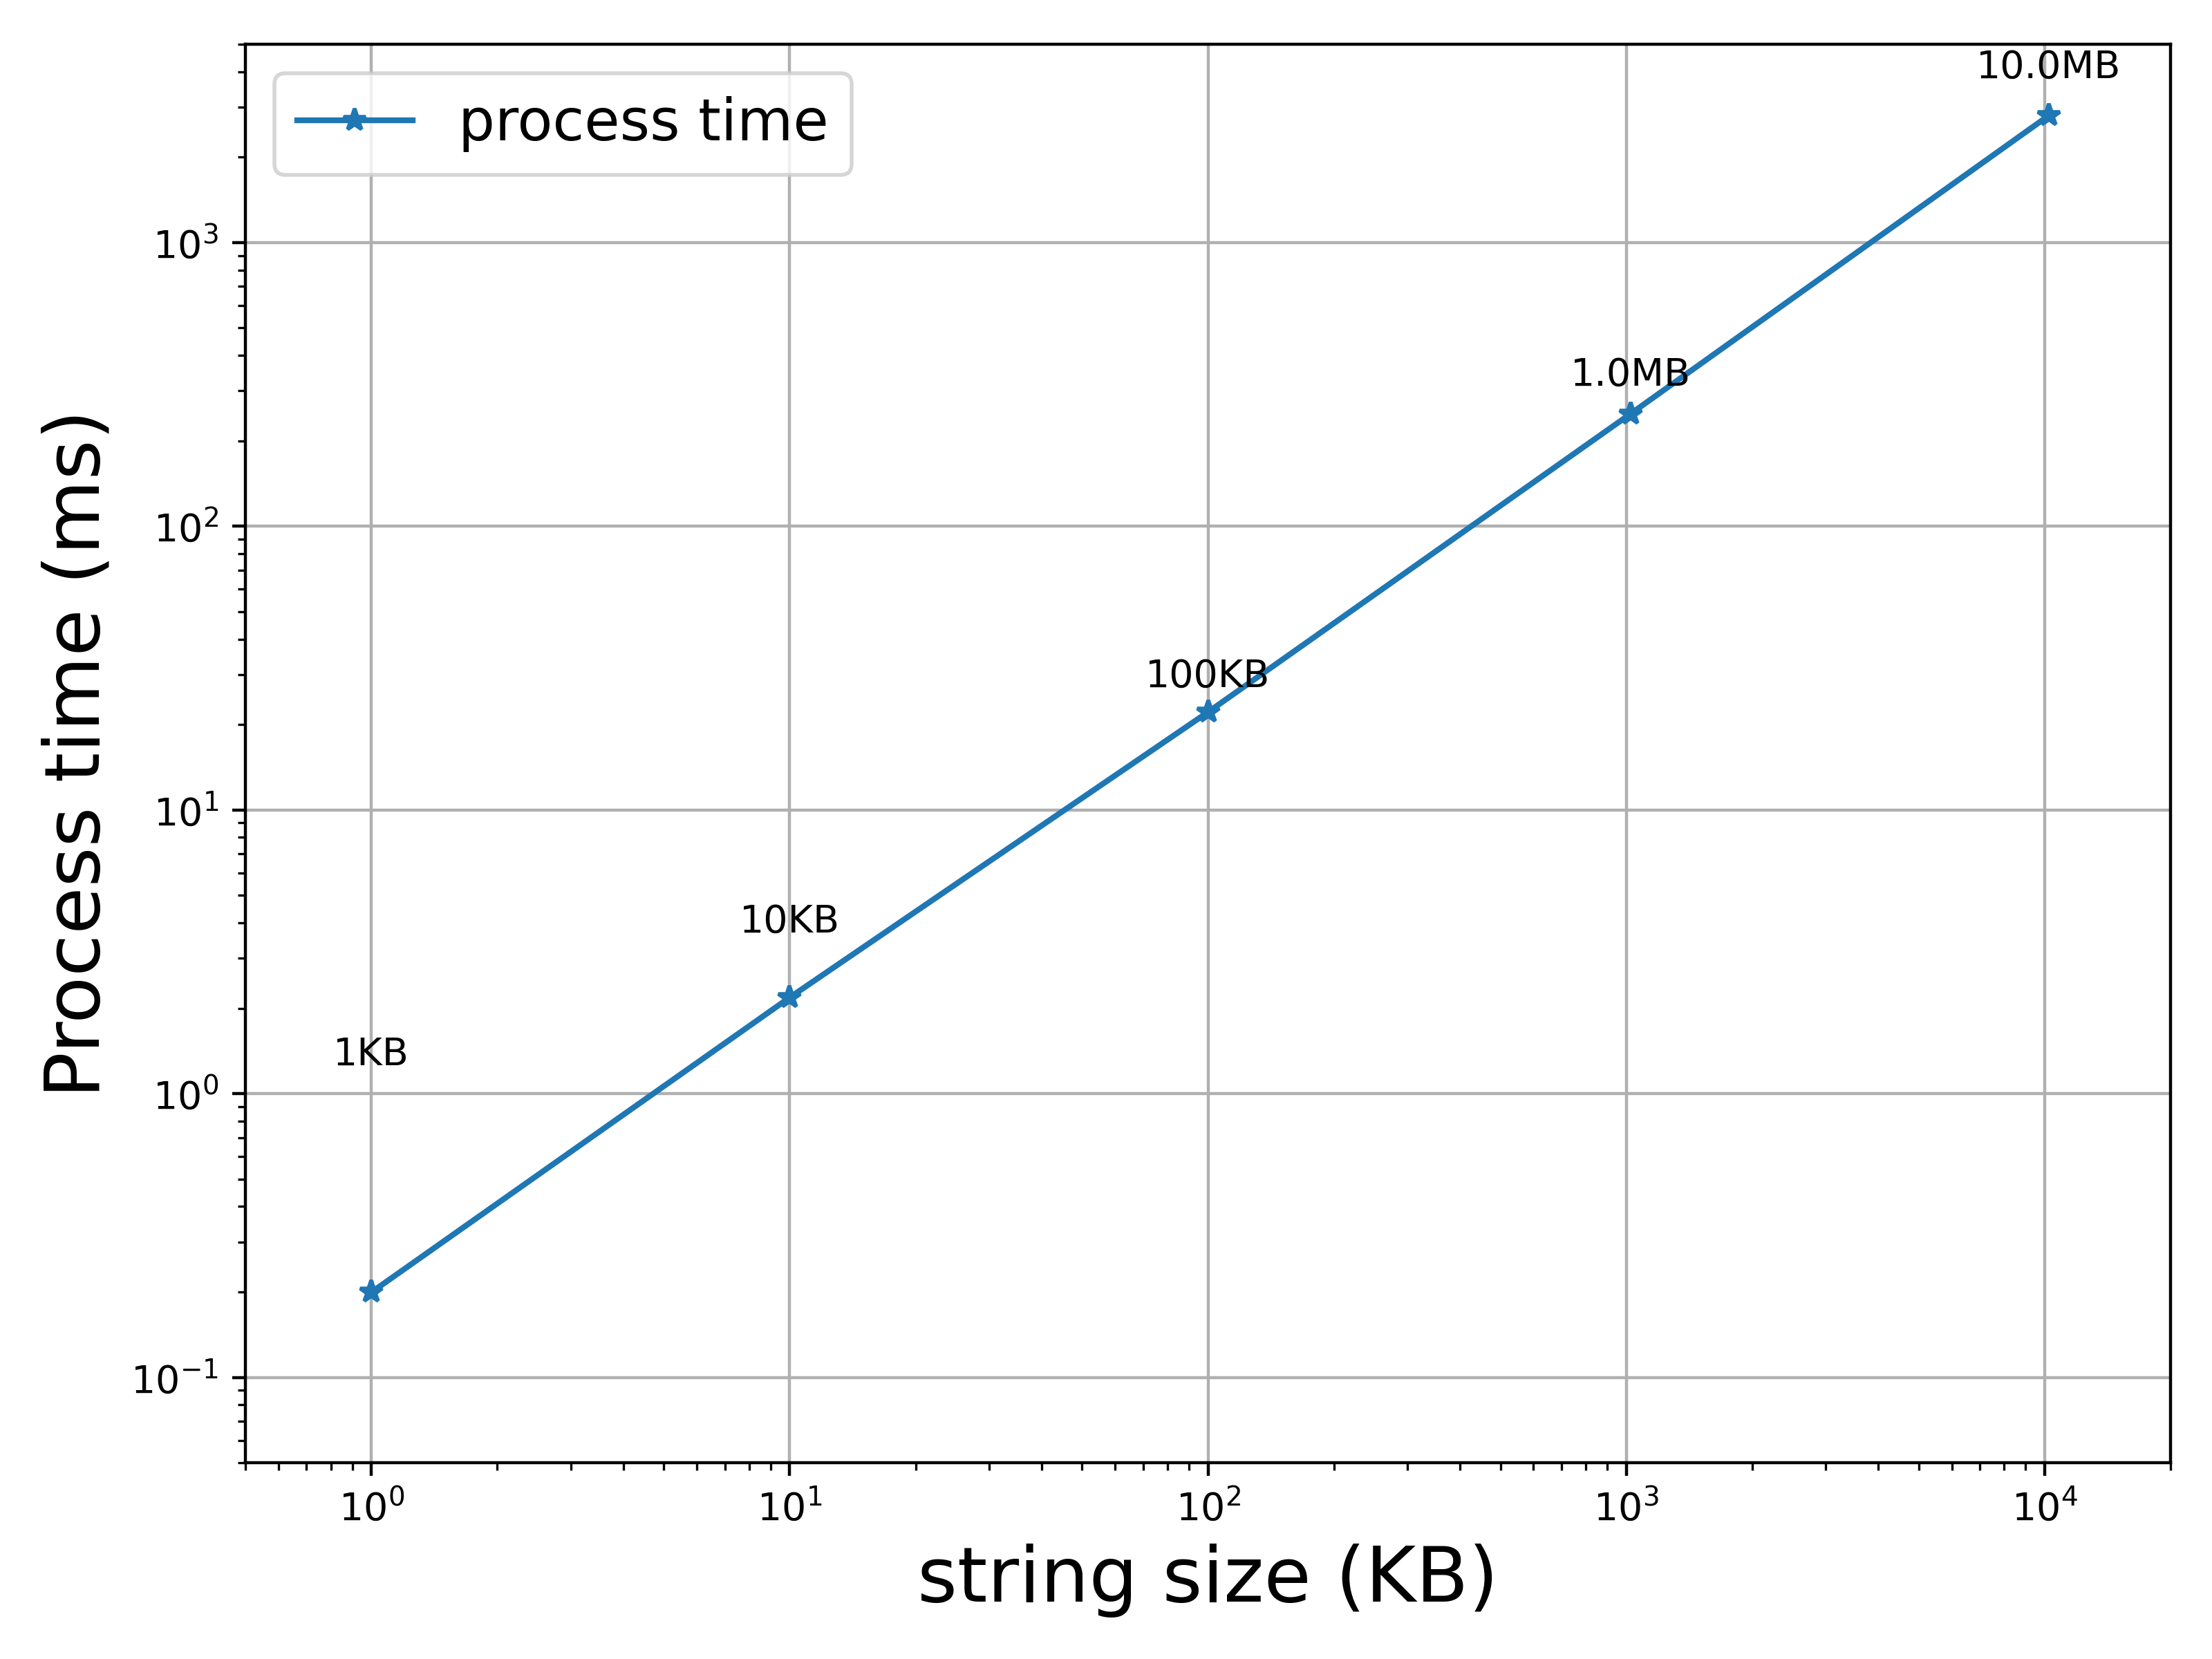
\includegraphics[width=\textwidth]{figures/tests/proportional_tests/Average_string_messages_receiving_time_of_100_tests_1KB_to_10MB.png} 
        \caption{} \label{fig: proportional-stringsize-b}
    \end{subfigure} 

    \caption{Average delay of sending and receiving a string message varied from 1KB 
    to 10MB for 100 times between 2 clients. (\subref{fig: proportional-stringsize-c}) Messages clientS sent forward, 
    (\subref{fig: proportional-stringsize-d}) response messages from clientR, 
    (\subref{fig: proportional-stringsize-a}) process time of massages sent forward 
    and (\subref{fig: proportional-stringsize-b}) process time of massages respond. 
    \label{fig: proportional-stringsize}}
\end{figure}

\subsubsection{Increasing image message length}
In addition to string, images are also frequently tranported between different agents. 
However, unlike most string messages, image size could be significantly larger 
and even up to over 100MB (raw images). Moreover, the agents ID or message priority 
information should also be included in the message. Therefore, the image should 
be first jsonified with necessary information and then sent to the server. 
The tests for images are done similar to the string message, with an image size 
varies from 1KB to 100MB. 


In fig.\ref{fig: proportional-imagesize-a} and \ref{fig: proportional-imagesize-b} 
again shows the linear dependency of latency and jsonified image size. 
Although the image test results in a 
transmisson time from 1KB to 10MB message length similar to string test, 
there is a huge difference in terms of process time between both. By comparing the 
fig.\ref{fig: proportional-stringsize-c} with \ref{fig: proportional-imagesize-c} 
and fig.\ref{fig: proportional-stringsize-d} with \ref{fig: proportional-imagesize-d}, 
the server process time of string messages is much higher than that for the 
image message. Meanwhile, due to the additional overhead of json format, the network 
delay of string messages is relative smaller than image messages. 


A possible reason for the larger process time for string is that, a string message 
received by server must be processed twice: splitting the message to extract the client 
ID and recombining it for further transport. Meanwhile a jsonified image will only be 
processed once to extract the client information and the original json file will be 
futher transported directly.     
\begin{figure}[htb]
        \centering
    \begin{subfigure}{0.49\textwidth}
        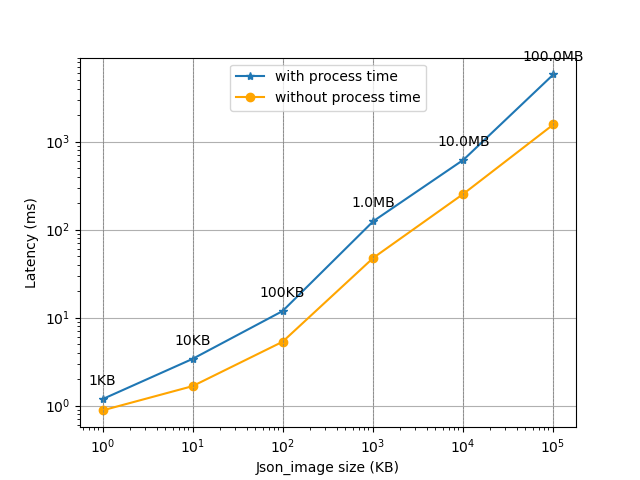
\includegraphics[width=\textwidth]{figures/tests/proportional_tests/log_Average_json_image_messages_sending_time_of_100_tests_1KB_to_100MB.png}\hfill 
        \caption{} \label{fig: proportional-imagesize-c}
    \end{subfigure}
    \begin{subfigure}{0.49\textwidth}
        \centering
        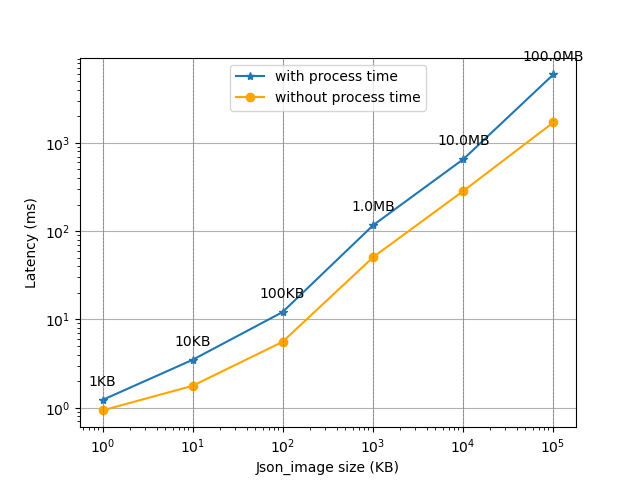
\includegraphics[width=\textwidth]{figures/tests/proportional_tests/log_Average_json_image_messages_receiving_time_of_100_tests_1KB_to_100MB.png}\hfill 
        \caption{} \label{fig: proportional-imagesize-d}
    \end{subfigure}
    \begin{subfigure}{0.49\textwidth}
        \centering
        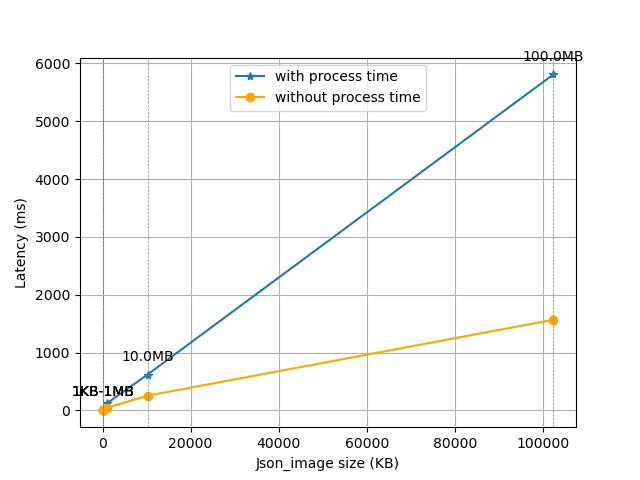
\includegraphics[width=\textwidth]{figures/tests/proportional_tests/Average_json_image_messages_sending_time_of_100_tests_1KB_to_100MB.png}\hfill 
        \caption{} \label{fig: proportional-imagesize-a}
    \end{subfigure}
    \begin{subfigure}{0.49\textwidth}
        \centering
        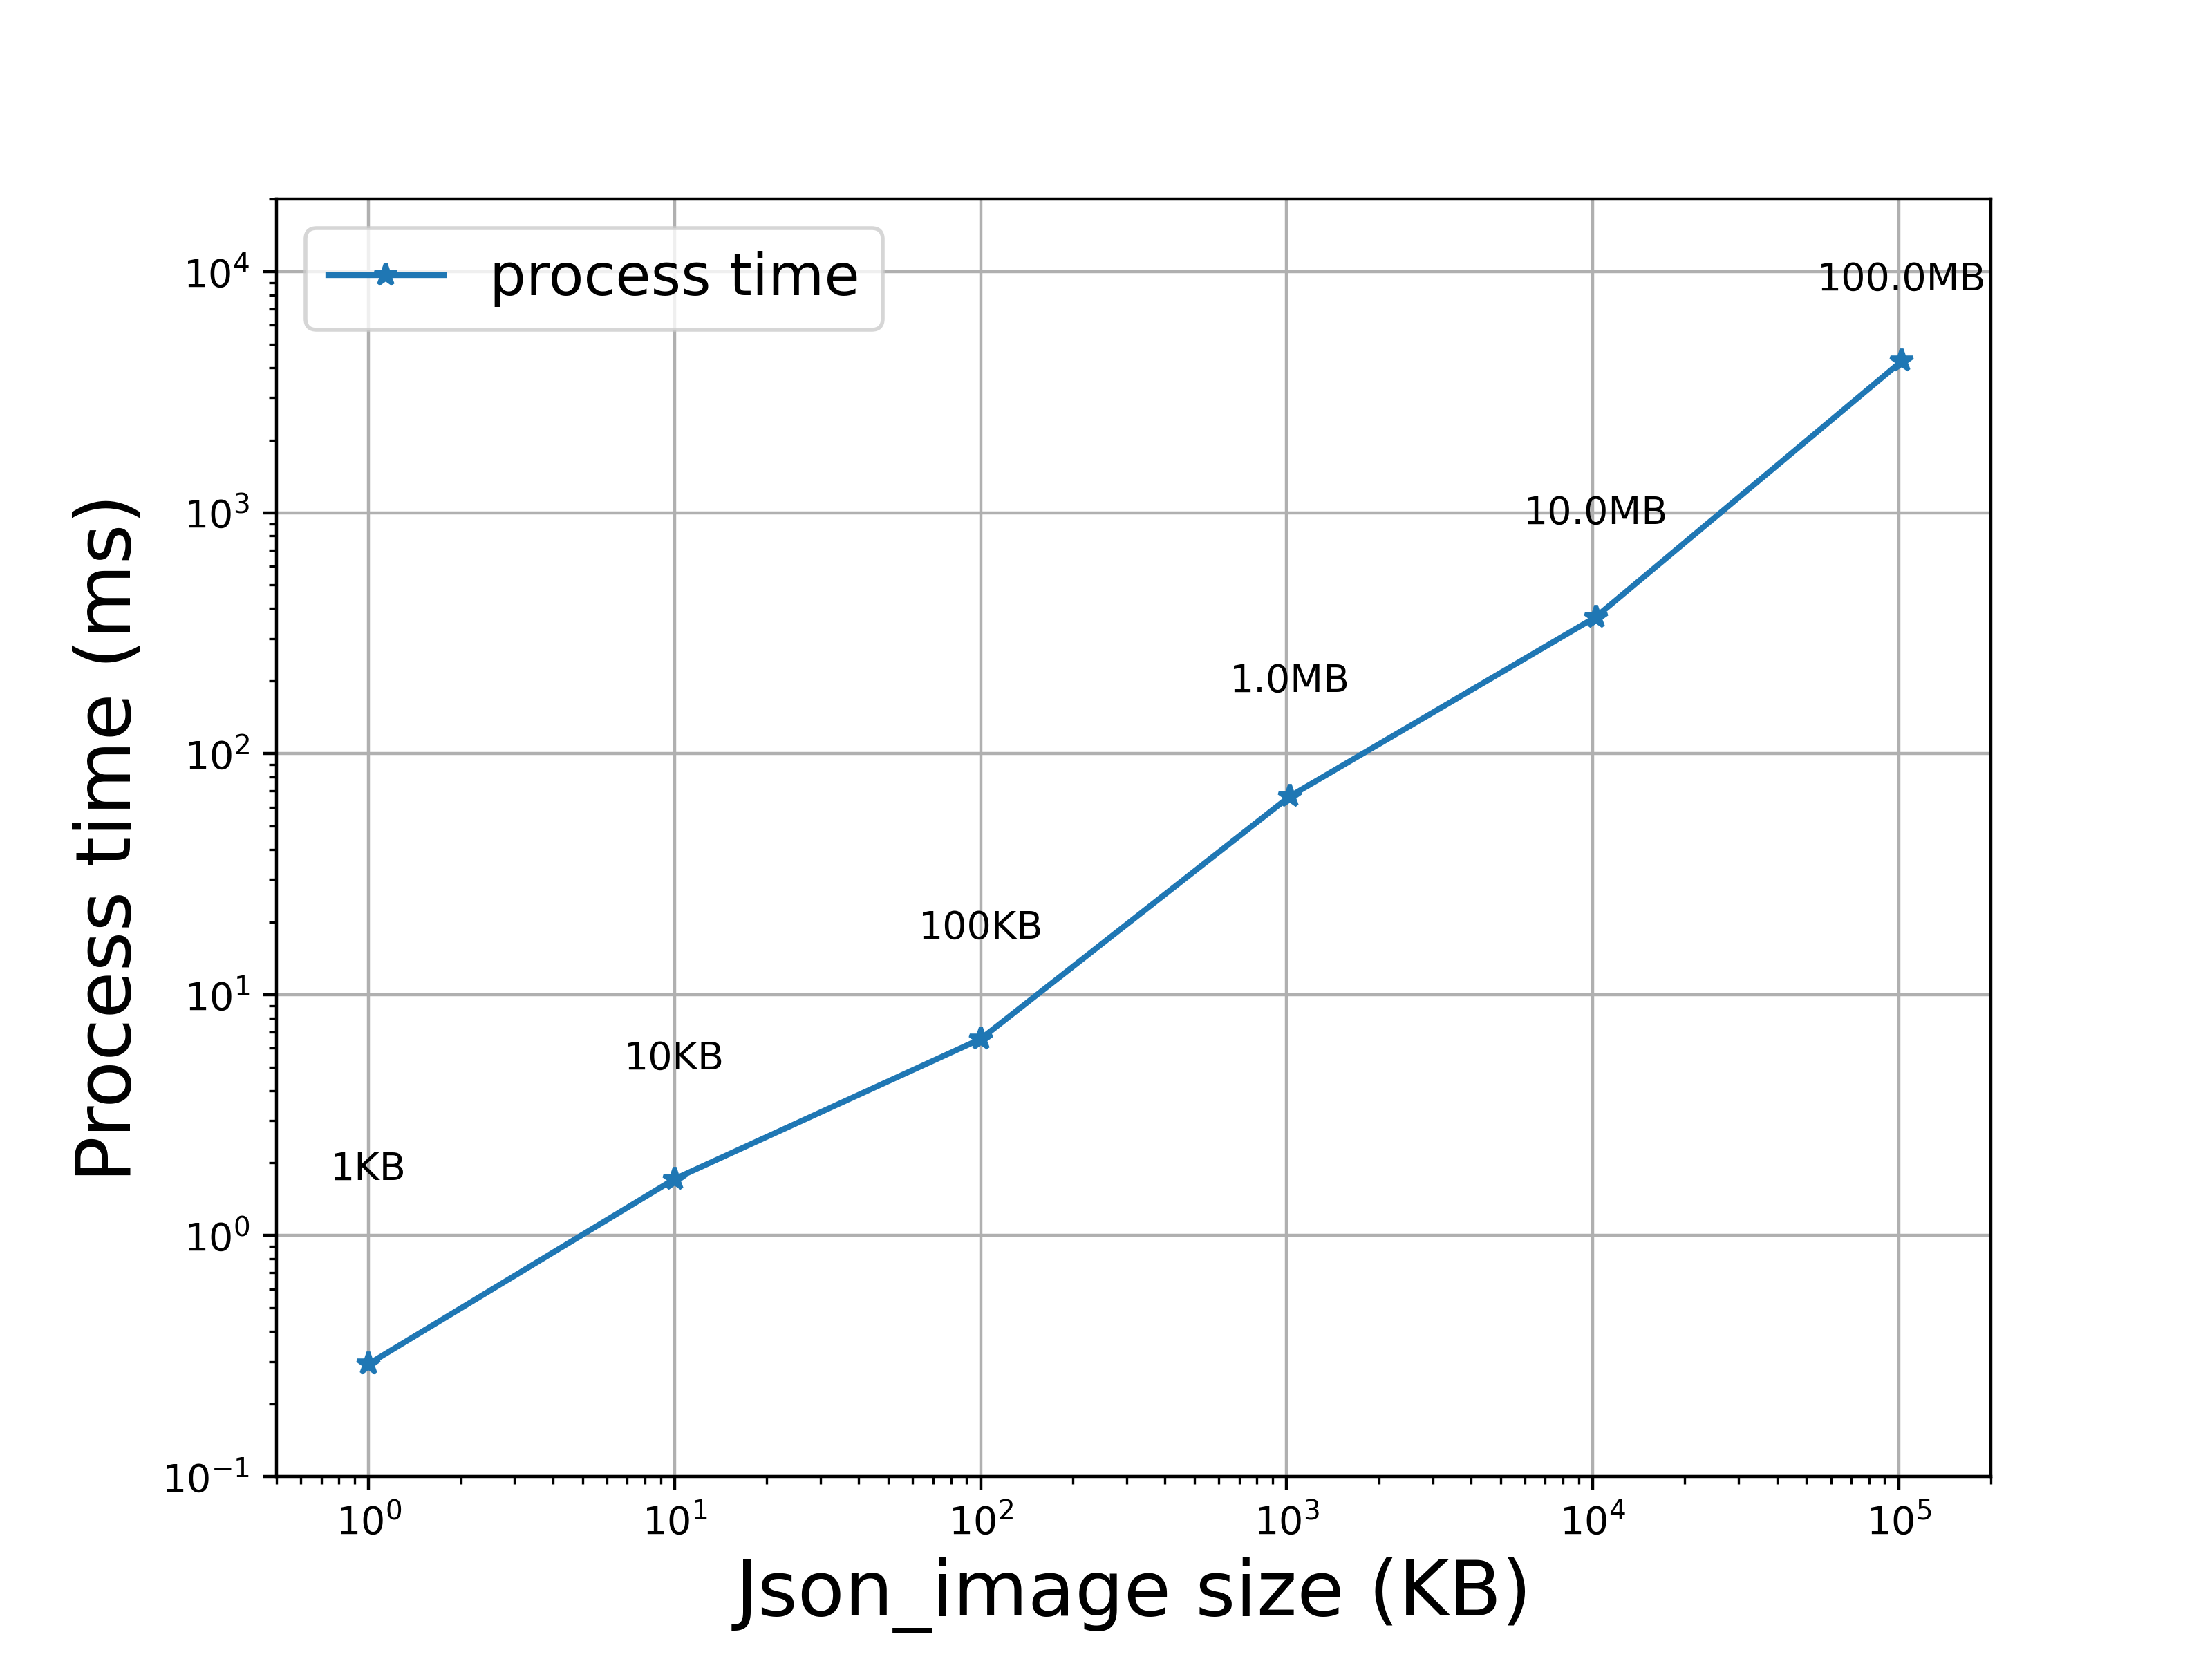
\includegraphics[width=\textwidth]{figures/tests/proportional_tests/Average_json_image_messages_receiving_time_of_100_tests_1KB_to_100MB.png}\hfill 
        \caption{} \label{fig: proportional-imagesize-b}
    \end{subfigure}

    \caption{Average delay of sending and receiving a jsonified image message varied from 1KB 
    to 100MB for 100 times between 2 clients. (\subref{fig: proportional-imagesize-c}) 
    Messages clientS sent forward in log form, 
    (\subref{fig: proportional-imagesize-d}) response messages from clientR in log form, 
    (\subref{fig: proportional-imagesize-a}) process time of messages sent forward  
    and (\subref{fig: proportional-imagesize-b}) process time of response messages from clientR. 
    \label{fig: proportional-imagesize}}
\end{figure}


\subsection{Test results of WebSocket and \gls{http}} \label{chap: Result-RestFUL_WS}
After testing the performance of the WebSocket based communication system, 
it will be interesting to see whether the other application layer protocols with 
different message transport mechanism will have a similar or completely different 
performance under the same conditions. As demonstrated from the 
fig.\ref{fig: MsgConceptual}, \gls{http} is designed for message 
transfer in both directions, and therefore more comparable with WebSocket among the others. 
As a result, a \gls{http} based interface RESTful API is designed under the similar architecture 
as WebSocket and tested under the same condition of the WebSocket string test in 
section \ref{chap: Result-Internal-string}. By comparing 
fig.\ref{fig: proportional-stringsize} with fig.\ref{fig: proportional-rest-stringsize}, 
it is obvious that the process time of string messages is higher and 
grows faster in a WebSocket server than RESTful API server. The difference may 
results in the prioritization and data processing mechanisms in WebSocket server, 
while RESTful API server is only designed with basic message POST and GET 
mechanism. However, the data transmission time between both is more comparable. 
First of all, both of them reflect the fit of the model with the coefficient 
of determination closes to one, which is namely: 


    \begin{align}
        R^{2} &= 1-\frac{RSS}{TSS}\\
        \text{Where} \nonumber\\
        RSS & = \text{sum of squared residuals} \nonumber\\
        TSS & = \text{total sum of squares}\nonumber
    \end{align}

meaning that the model fits the data well.





Secondly, the transmission time of both is similar 
with respect to the same string message length (RESTful has slightly higher latency), 
with a difference of 0.01ms to few milliseconds, which grows over 
message size.   

Therefore, WebSocket is proven to be more appropriate for real time message 
transfer, which is essential for an agent based system.


\begin{figure}[htb]
    \begin{subfigure}[b]{0.49\textwidth}
        \centering
        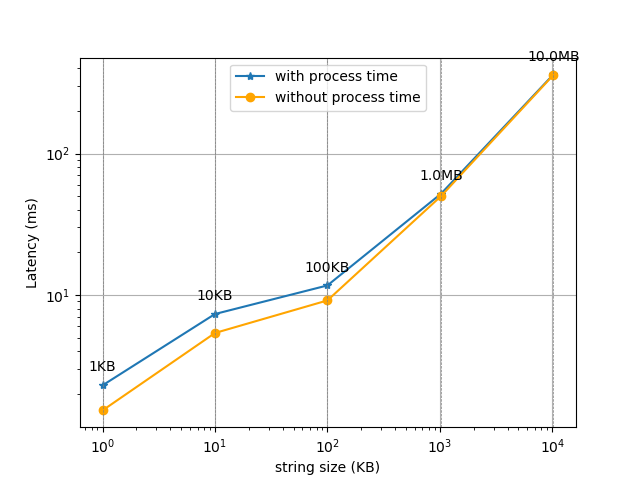
\includegraphics[width=\textwidth]{figures/tests/proportional_tests/Rest_log_Average_string_messages_sending_time_of_100_tests.png}\hfill 
        \caption{} \label{fig: proportional-rest-stringsize-c}
    \end{subfigure}
    \begin{subfigure}[b]{0.49\textwidth}
        \centering
        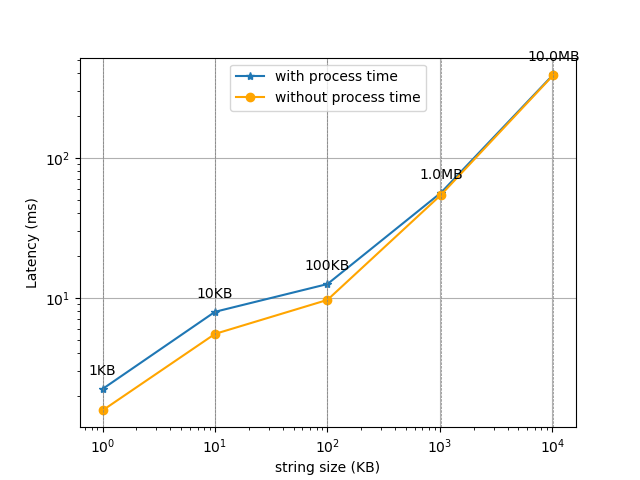
\includegraphics[width=\textwidth]{figures/tests/proportional_tests/Rest_log_Average_string_messages_receiving_time_of_100_tests.png}\hfill 
        \caption{} \label{fig: proportional-rest-stringsize-d}
    \end{subfigure}

    \begin{subfigure}[b]{0.49\textwidth}
        \centering
        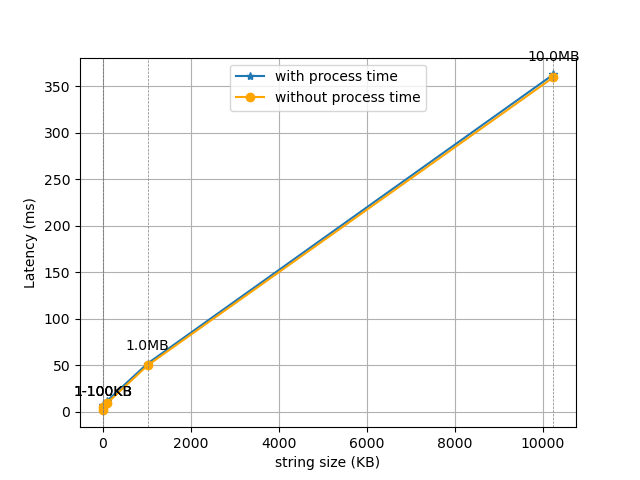
\includegraphics[width=\textwidth]{figures/tests/proportional_tests/Rest_Average_string_messages_sending_time_of_100_tests.png}\hfill 
        \caption{} \label{fig: proportional-rest-stringsize-a}
    \end{subfigure}
    \begin{subfigure}[b]{0.49\textwidth}
        \centering
        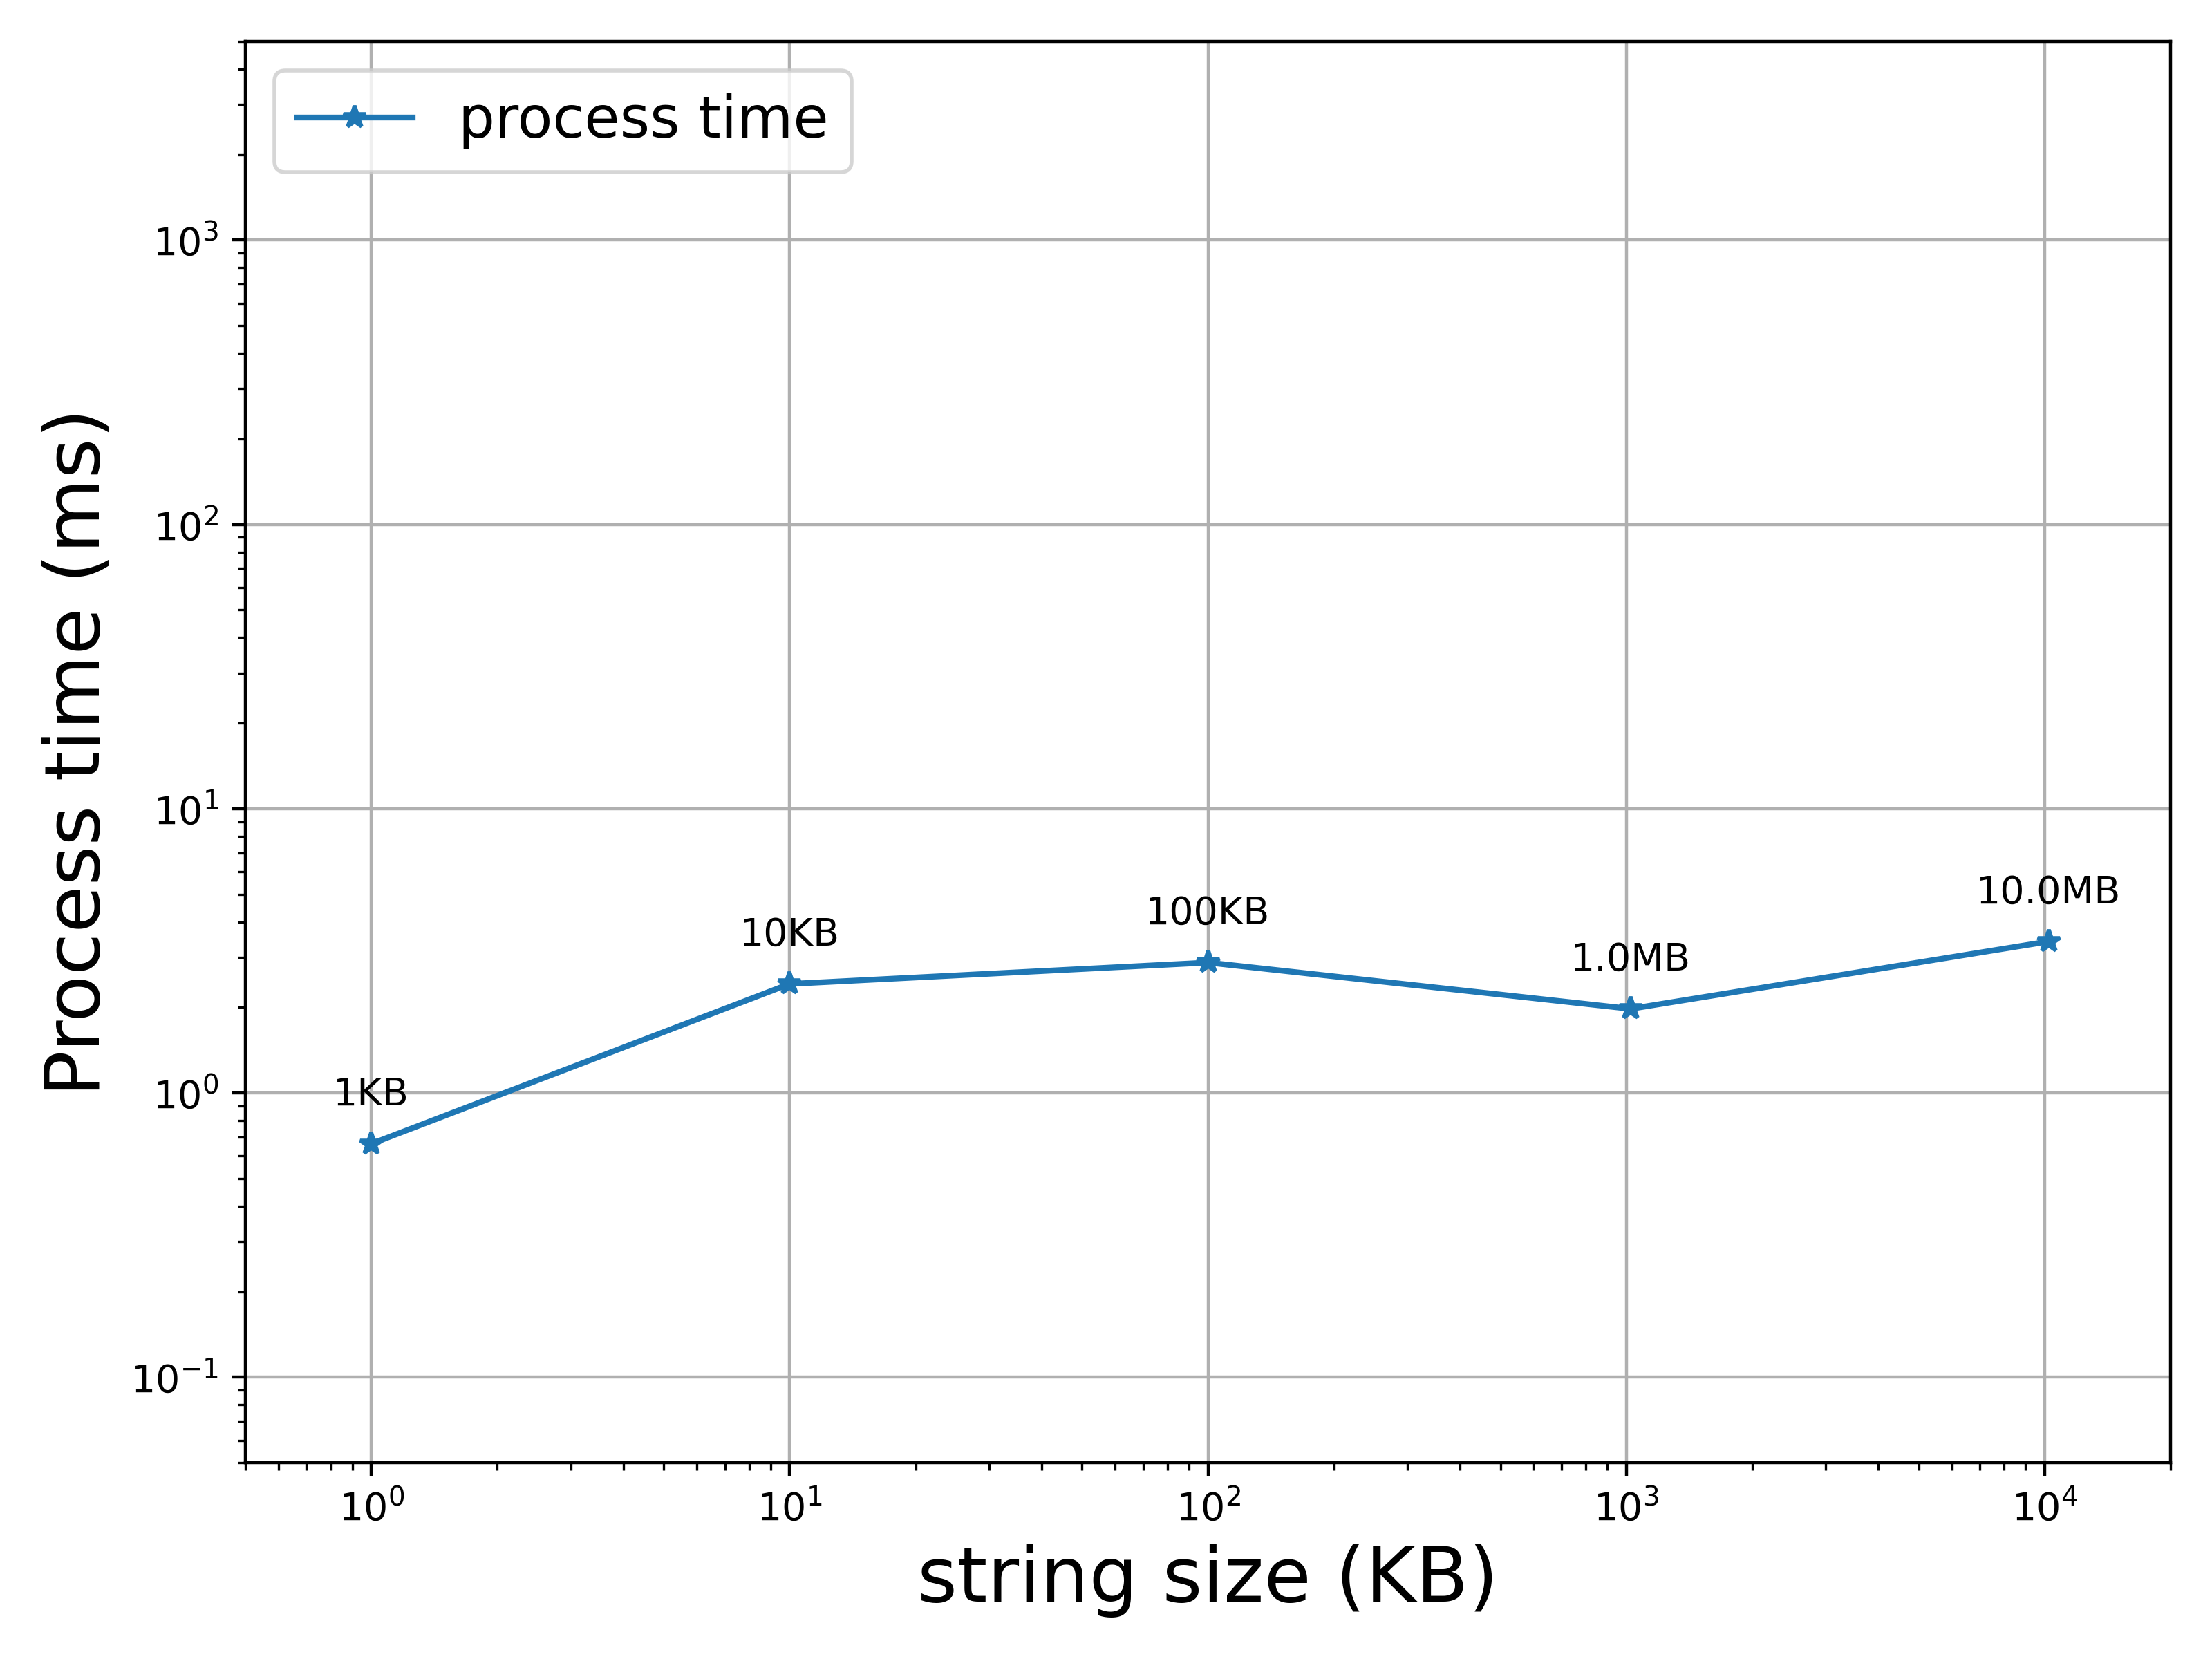
\includegraphics[width=\textwidth]{figures/tests/proportional_tests/Rest_Average_string_messages_receiving_time_of_100_tests.png}\hfill 
        \caption{} \label{fig: proportional-rest-stringsize-b}
    \end{subfigure}
    
    \caption{RESTful API: Average delay of sending and receiving a string message varied from 1KB 
    to 10MB for 100 times between 2 clients. (\subref{fig: proportional-rest-stringsize-c}) 
    Messages clientS sent forward, 
    (\subref{fig: proportional-rest-stringsize-d}) response messages from clientR, 
    (\subref{fig: proportional-rest-stringsize-a}) process time of messages sent forward 
    and (\subref{fig: proportional-rest-stringsize-b}) process time of messages respond. 
    \label{fig: proportional-rest-stringsize}}
\end{figure}





\subsection{Test results of message prioritization of a WebSocket server in various 
performance testing} \label{chap: Result-priority}
Apart from the consideration of speed, robustness, reliability and application size in an agent 
communication system, the server which serves as a \gls{ca} should have addtional 
functionalities rather than pure message transport. As listed in tab.\ref{tab:designPatterns}, 
the \gls{ca} should focus on the design of a communication interface, which should be able to 
process various messages with different data types (e.g., jsonified images), handle a large 
number of agents connections and prioritize the incoming messages. In the following sections, 
the performance of server handling message prioritization will be tested and further discussed.  

\subsubsection{Measurgin method}
In order to verify the prioritization mechanism of the server, a delay of 1s should be added to the 
non-prioritized message processing. In the test, two kinds of messages are sent conccurently to the server, 
the normal and the critical messages. If more than one message with different priority levels 
enter the server simultaneously, the critical messages should be processed first. The add up of 
delay also reflects the real world scenarios: if a critical message representing an emergent stop 
or a task with higher priority in production comes in, every other processe in the server 
should wait until the critical message is sent. 

\subsubsection{String message priority test}
The first string priority test is done for 10 clients. The following fig.\ref{fig: priority-10clients-a} 
and \ref{fig: priority-10clients-b} shows the mean \gls{rtt} 
that a non-prioritized and prioritized message being sent forward and back separately for 100 times.
In fig.\ref{fig: priority-10clients-a}, the mean \gls{rtt} for client1 to client10 in both directions 
varies from 0.63ms to 1.09ms, 
which fullfills the near real time requirement(quote) for production process. 
The fig.\ref{fig: priority-10clients-b} on the other hand, 
presents the timing differences of normal messages as a group and critical messages as control group. 
In the test, all clients deliver normal messages except for client10. That means, whenever a critical 
message from client10 arrives, the server will pause the other processes for 1s and handle the 
critical message immediately. In the test, the mean \gls{rtt} for client10 is less than 1ms. 
In contrast, clients such as client1 through client5 and client9 experience 
significantly higher RTTs, sometimes reaching several hundred milliseconds, which 
has verified the assumption of message prioritization. It is worth mentioning that, due to the concurrent 
nature of the asyncio package in the WebSocket server design, each client will be executed 
one after another, different from parallel processing. That means, some messages may never be paused 
if the clients execution process is not synchronized and coordinated explicitly. 

\begin{sidewaysfigure}[htb]
    \centering
    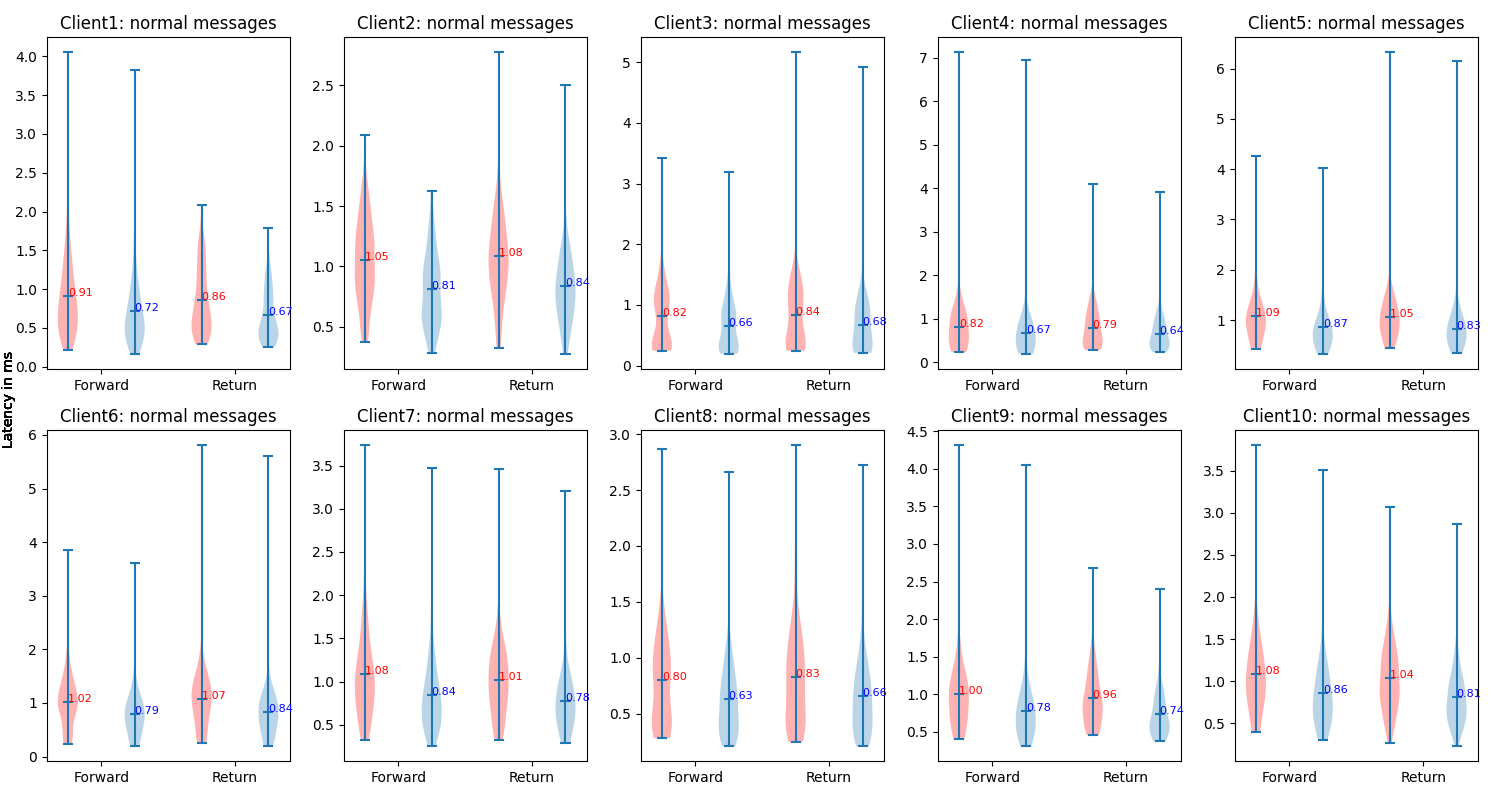
\includegraphics[width=\textheight]{figures/tests/priority_tests/violin_10clients_string_non_priority.png}\hfill 
    \caption{Tests for mean \gls{rtt} of forward and return non-prioritized string messages between 10 clients 
    and clientR for 100 times. The blue violin represents the average data transmission time and the red violin 
    respresent mean \gls{rtt}.} \label{fig: priority-10clients-a}
\end{sidewaysfigure}
\begin{sidewaysfigure}[htb]
    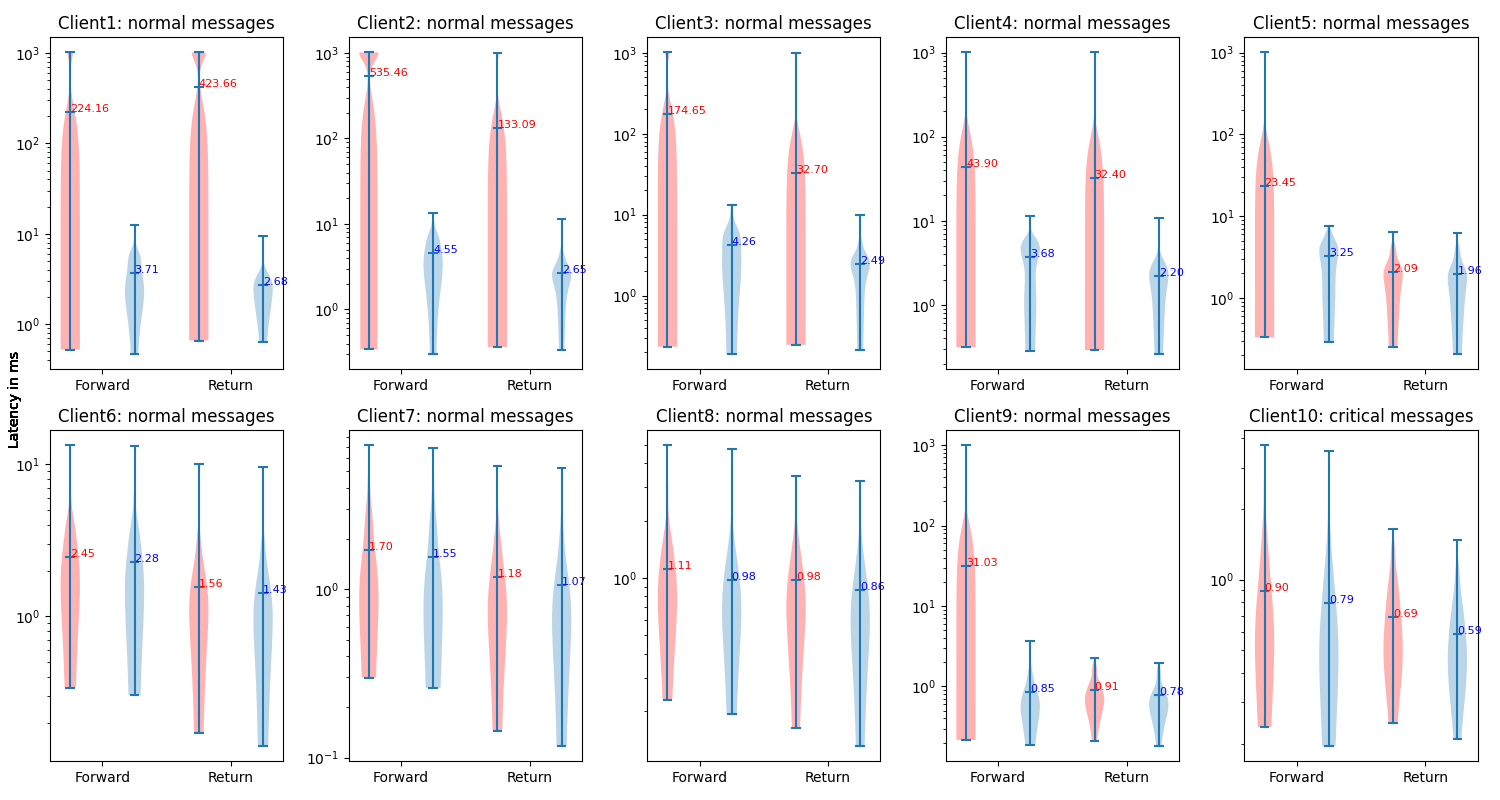
\includegraphics[width=\textheight]{figures/tests/priority_tests/log_violin_10clients_string_priority.png}\hfill 
    \caption{Tests for mean \gls{rtt} of forward and return prioritized string messages between 10 clients 
    and clientR for 100 times. The blue violin represents the average data transmission time and the red violin 
    respresent mean \gls{rtt}.} \label{fig: priority-10clients-b}
\end{sidewaysfigure}



Together with the priority tests for 10 clients, there are similar tests performed in different scales. 
In all these tests, the number of clients varies from 2, 10 to 50. The test results 
of 2 clients can be found in \ref{chap: append-string-priority} fig.\ref{fig: priority-2clients-string}, 
and those for 50 clients in fig.\ref{fig: priority-50clients-string-a} to 
\ref{fig: priority-50clients-string-e}. For the string message priority test with 2 clients, 
it is clear that client1 sends messages with lower priority results in 
a much higher delay than client2 in both directions. As for the test with 50 clients, 
the test result is similar to those in the test for 10 clients. In the test, only the 
last client will send a critical message, while the other 49 clients with a normal message. 
This resulted in some clients being affected by the mechanism and greatly increasing delays, 
while client50 will always have a smallest \gls{rtt}.

\subsubsection{Image message priority test}
The same tests are also done for image message transport. Slightly different 
from string messages, the prioritization jsonified image file (image size: 33.4KB) 
will be performed 
after deserialization. In the image priority test, client1 to client10 will send an 
image to clientR, and receive a string message as response. In actual production,
a confirm string message will be sent back if the image message is successfully received 
by clientR. Therefore, this test can better reflect the time difference between 
different messages types in the actual production process, since mostly the actual 
string length will be much smaller than the image length. As shown in fig.\ref{fig: priority-10clients-c}, 
it proves that either the data transmission time or the server process time of a image message 
will be higher than a string message.


\begin{sidewaysfigure}[htb]
    \centering
    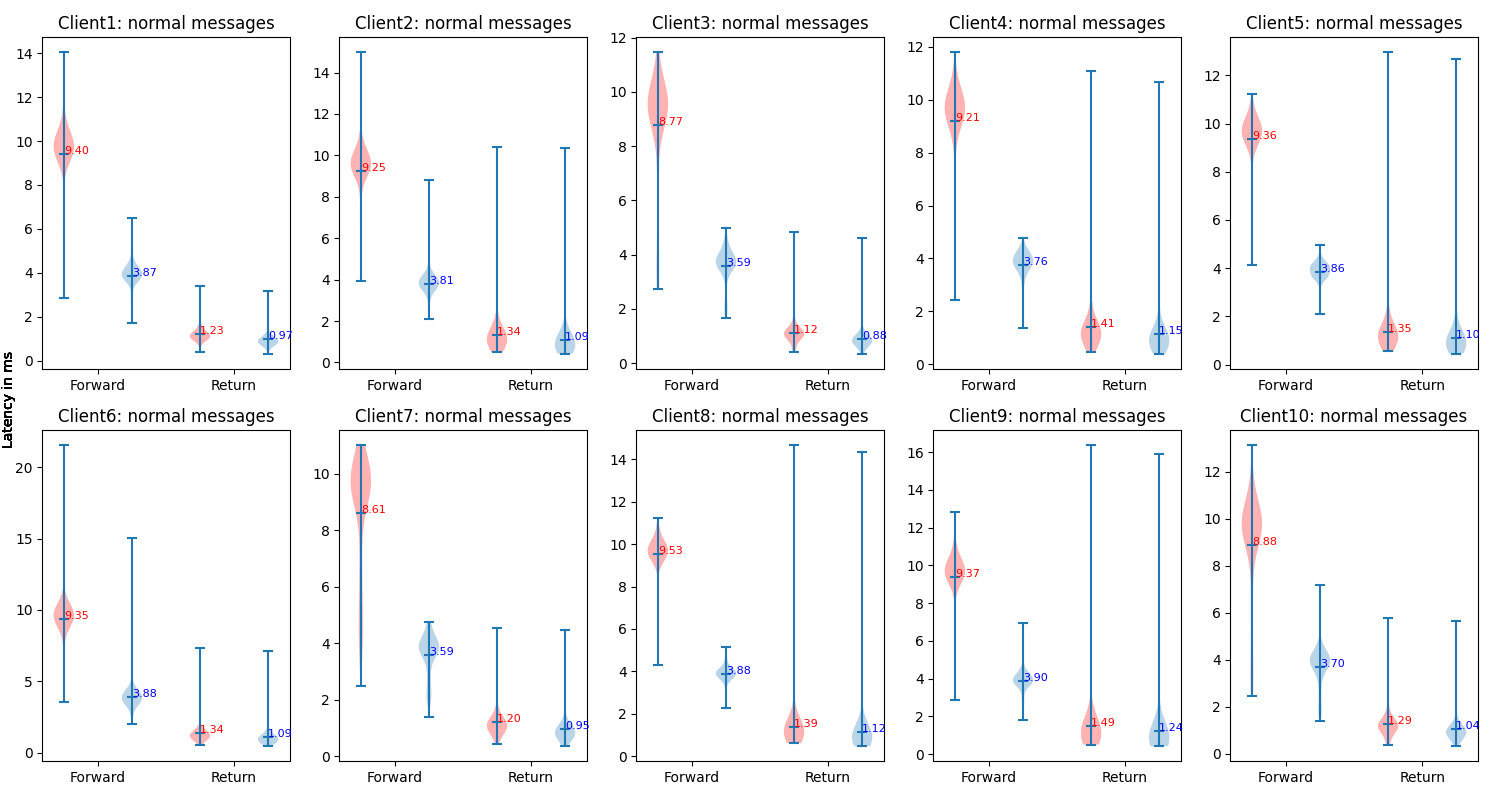
\includegraphics[width=\textheight]{figures/tests/priority_tests/violin_10clients_image_non_priority.png}\hfill 
    \caption{Tests for mean \gls{rtt} of non-prioritized forward image messages and return string messages between 10 clients 
    and clientR for 100 times. The blue violin represents the average data transmission time and the red violin 
    respresent mean \gls{rtt}.} \label{fig: priority-10clients-c}
\end{sidewaysfigure}


Another test (fig.\ref{fig: priority-10clients-d}) should be similar to the string message priority test (fig.\ref{fig: priority-10clients-b}), 
with 2, 10 and 50 clients sending images and receiving string messages as response 
from clientR. 
All client1 to client9 send a normal image message and meanwhile 
client10 sends a critical one to clientR. 
In the test, all image messages and only a part of the response string messages 
being sent trigger the prioritization mechanism.  In this, the latency for 
the prioritized string messages is very similar to previous test results
The reason might be that the larger the file size, the longer the transfer 
and processing time will required. The larger message length of images 
results in more data bytes 
that needs to be processed simultaneously, which involves the a higher number of 
message queuing and message prioritization in server. The same conclusion can be 
also made for the tests for 2 and 50 clients in \ref{chap: append-image-priority} fig.\ref{fig: priority-2clients-image} 
to \ref{fig: priority-50clients-image-e}.


\begin{sidewaysfigure}[htb]
    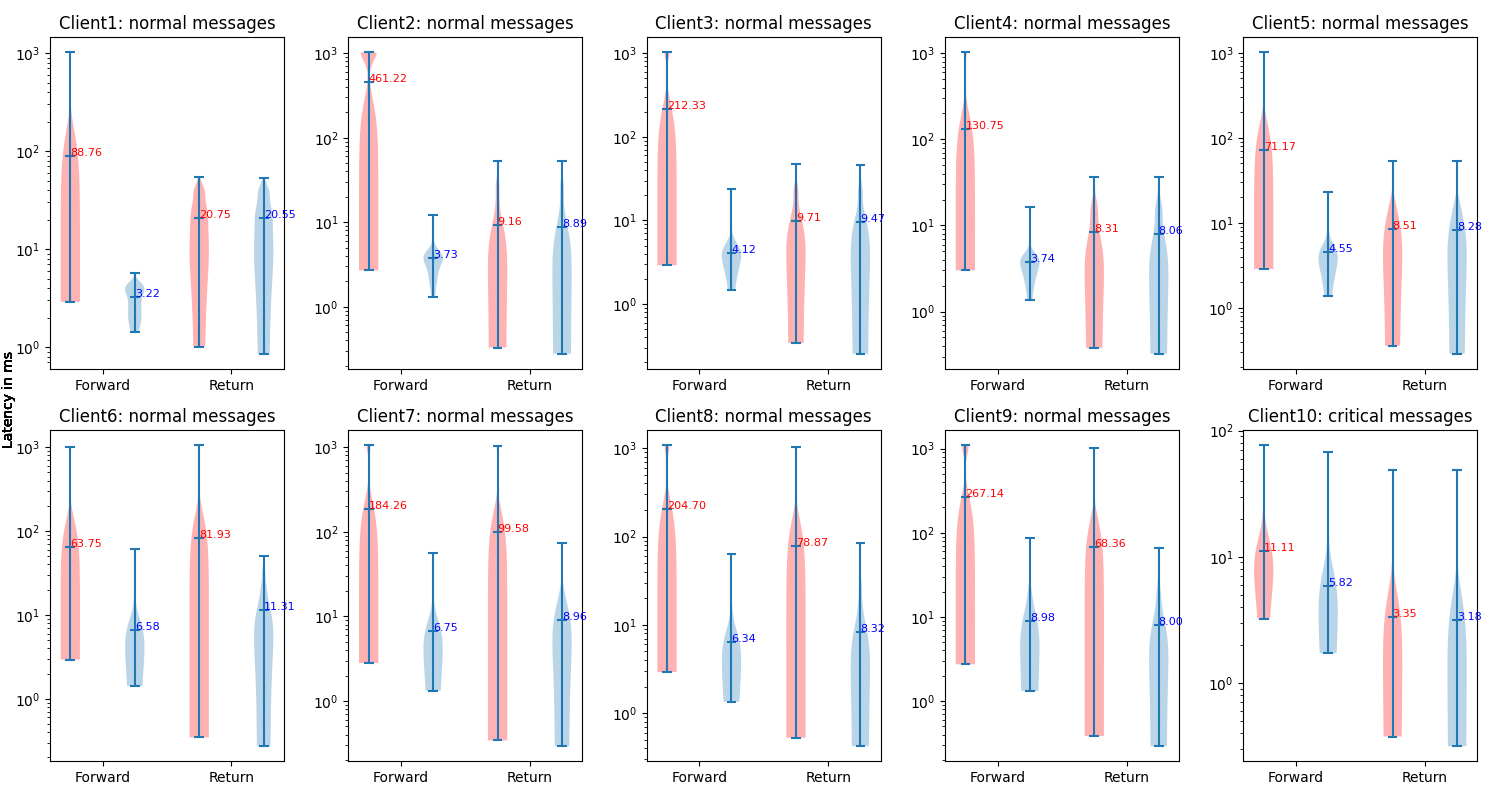
\includegraphics[width=\textheight]{figures/tests/priority_tests/log_violin_10clients_image_priority.png}\hfill 
    \caption{Tests for mean \gls{rtt} of prioritized forward image messages and return string messages between 10 clients 
    and clientR for 100 times. The blue violin represents the average data transmission time and the red violin 
    respresent mean \gls{rtt}.} \label{fig: priority-10clients-d}
\end{sidewaysfigure}


\subsection{Diagrams of WebSocket based \gls{mas} architecture under two use cases and test 
test results of BMW use case}\label{chap: Result-Internal-Usecase}
As listed earlier in form of pseudocode in section \ref{chap: Meth-WS-MAS}, 
the \gls{mas} architecture is designed for all use cases. In the code, a complete 
workflow from agents allocation to the sequenced based agents communication 
is designed for a standard production process in real world. For a better 
understanding of the workflow of both usecases, two diagrams are provided: 
fig.\ref{fig: sequence-diagram} shows a general workflow for a general 
use case diagram that can be applied to all use cases, 
and fig.\ref{fig: Flowchart-usecase} shows the actual workflow of the 
two use cases. 


In the general use case diagram (fig.\ref{fig: sequence-diagram}), the 
design for the \gls{mas} should be identical for all use cases except for 
the availability check and primitive execution parts (production processes) 
in the loop. The detailed 
program execution sequence is already described in section \ref{chap: Meth-WS-MAS}, 
something worth noting here is that, the sequence the production processes in the loop should 
be relevant to use cases, namely the customer requirements. That means, the sequence 
for tasks execution in the test should be more complex. Rather than a simple round trip 
between three agents, sometimes the Transport agent can receive orders from Storage agent 
and send orders to the Storage agent again to save time from the slow restocking of 
supermarket cell. However, the workflow in fig.\ref{fig: Flowchart-usecase} may 
it may be the best route in actual production based on its simplicity of agents 
communication design.  


\begin{figure}[htb]
    \centering
    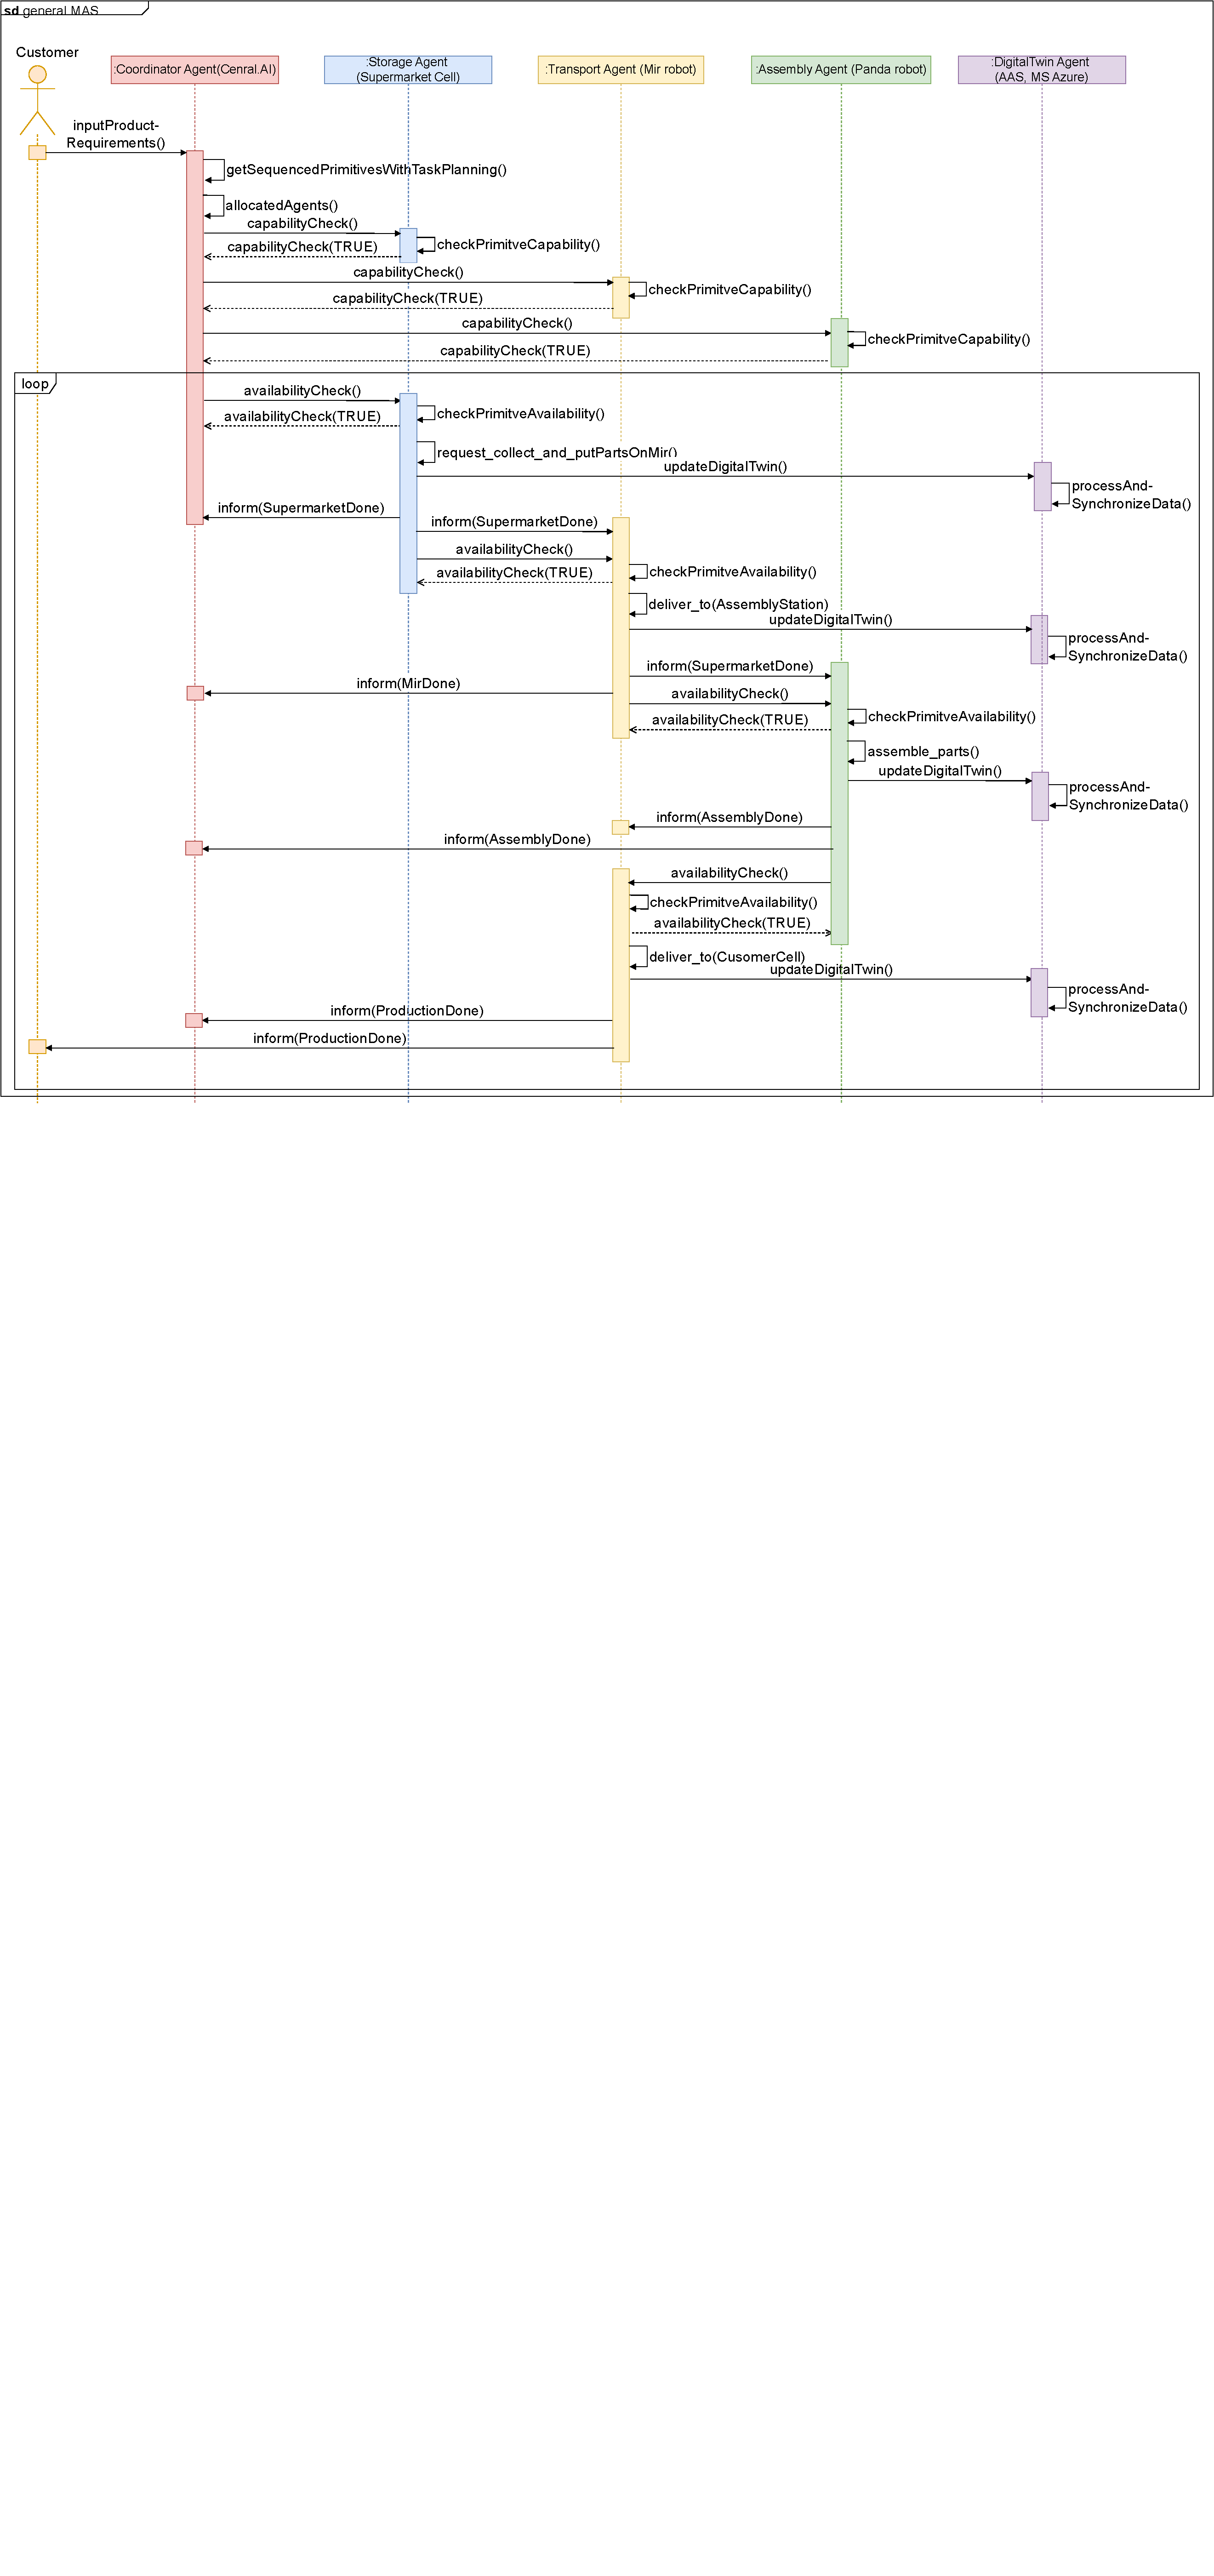
\includegraphics[width=\textwidth]{figures/tests/usecase/SequenceUsecases.pdf}\hfill 
    \caption{\gls{uml} general use case diagram of the \gls{mas} architecture.} 
    \label{fig: sequence-diagram}
\end{figure}


\begin{figure}[htb]
    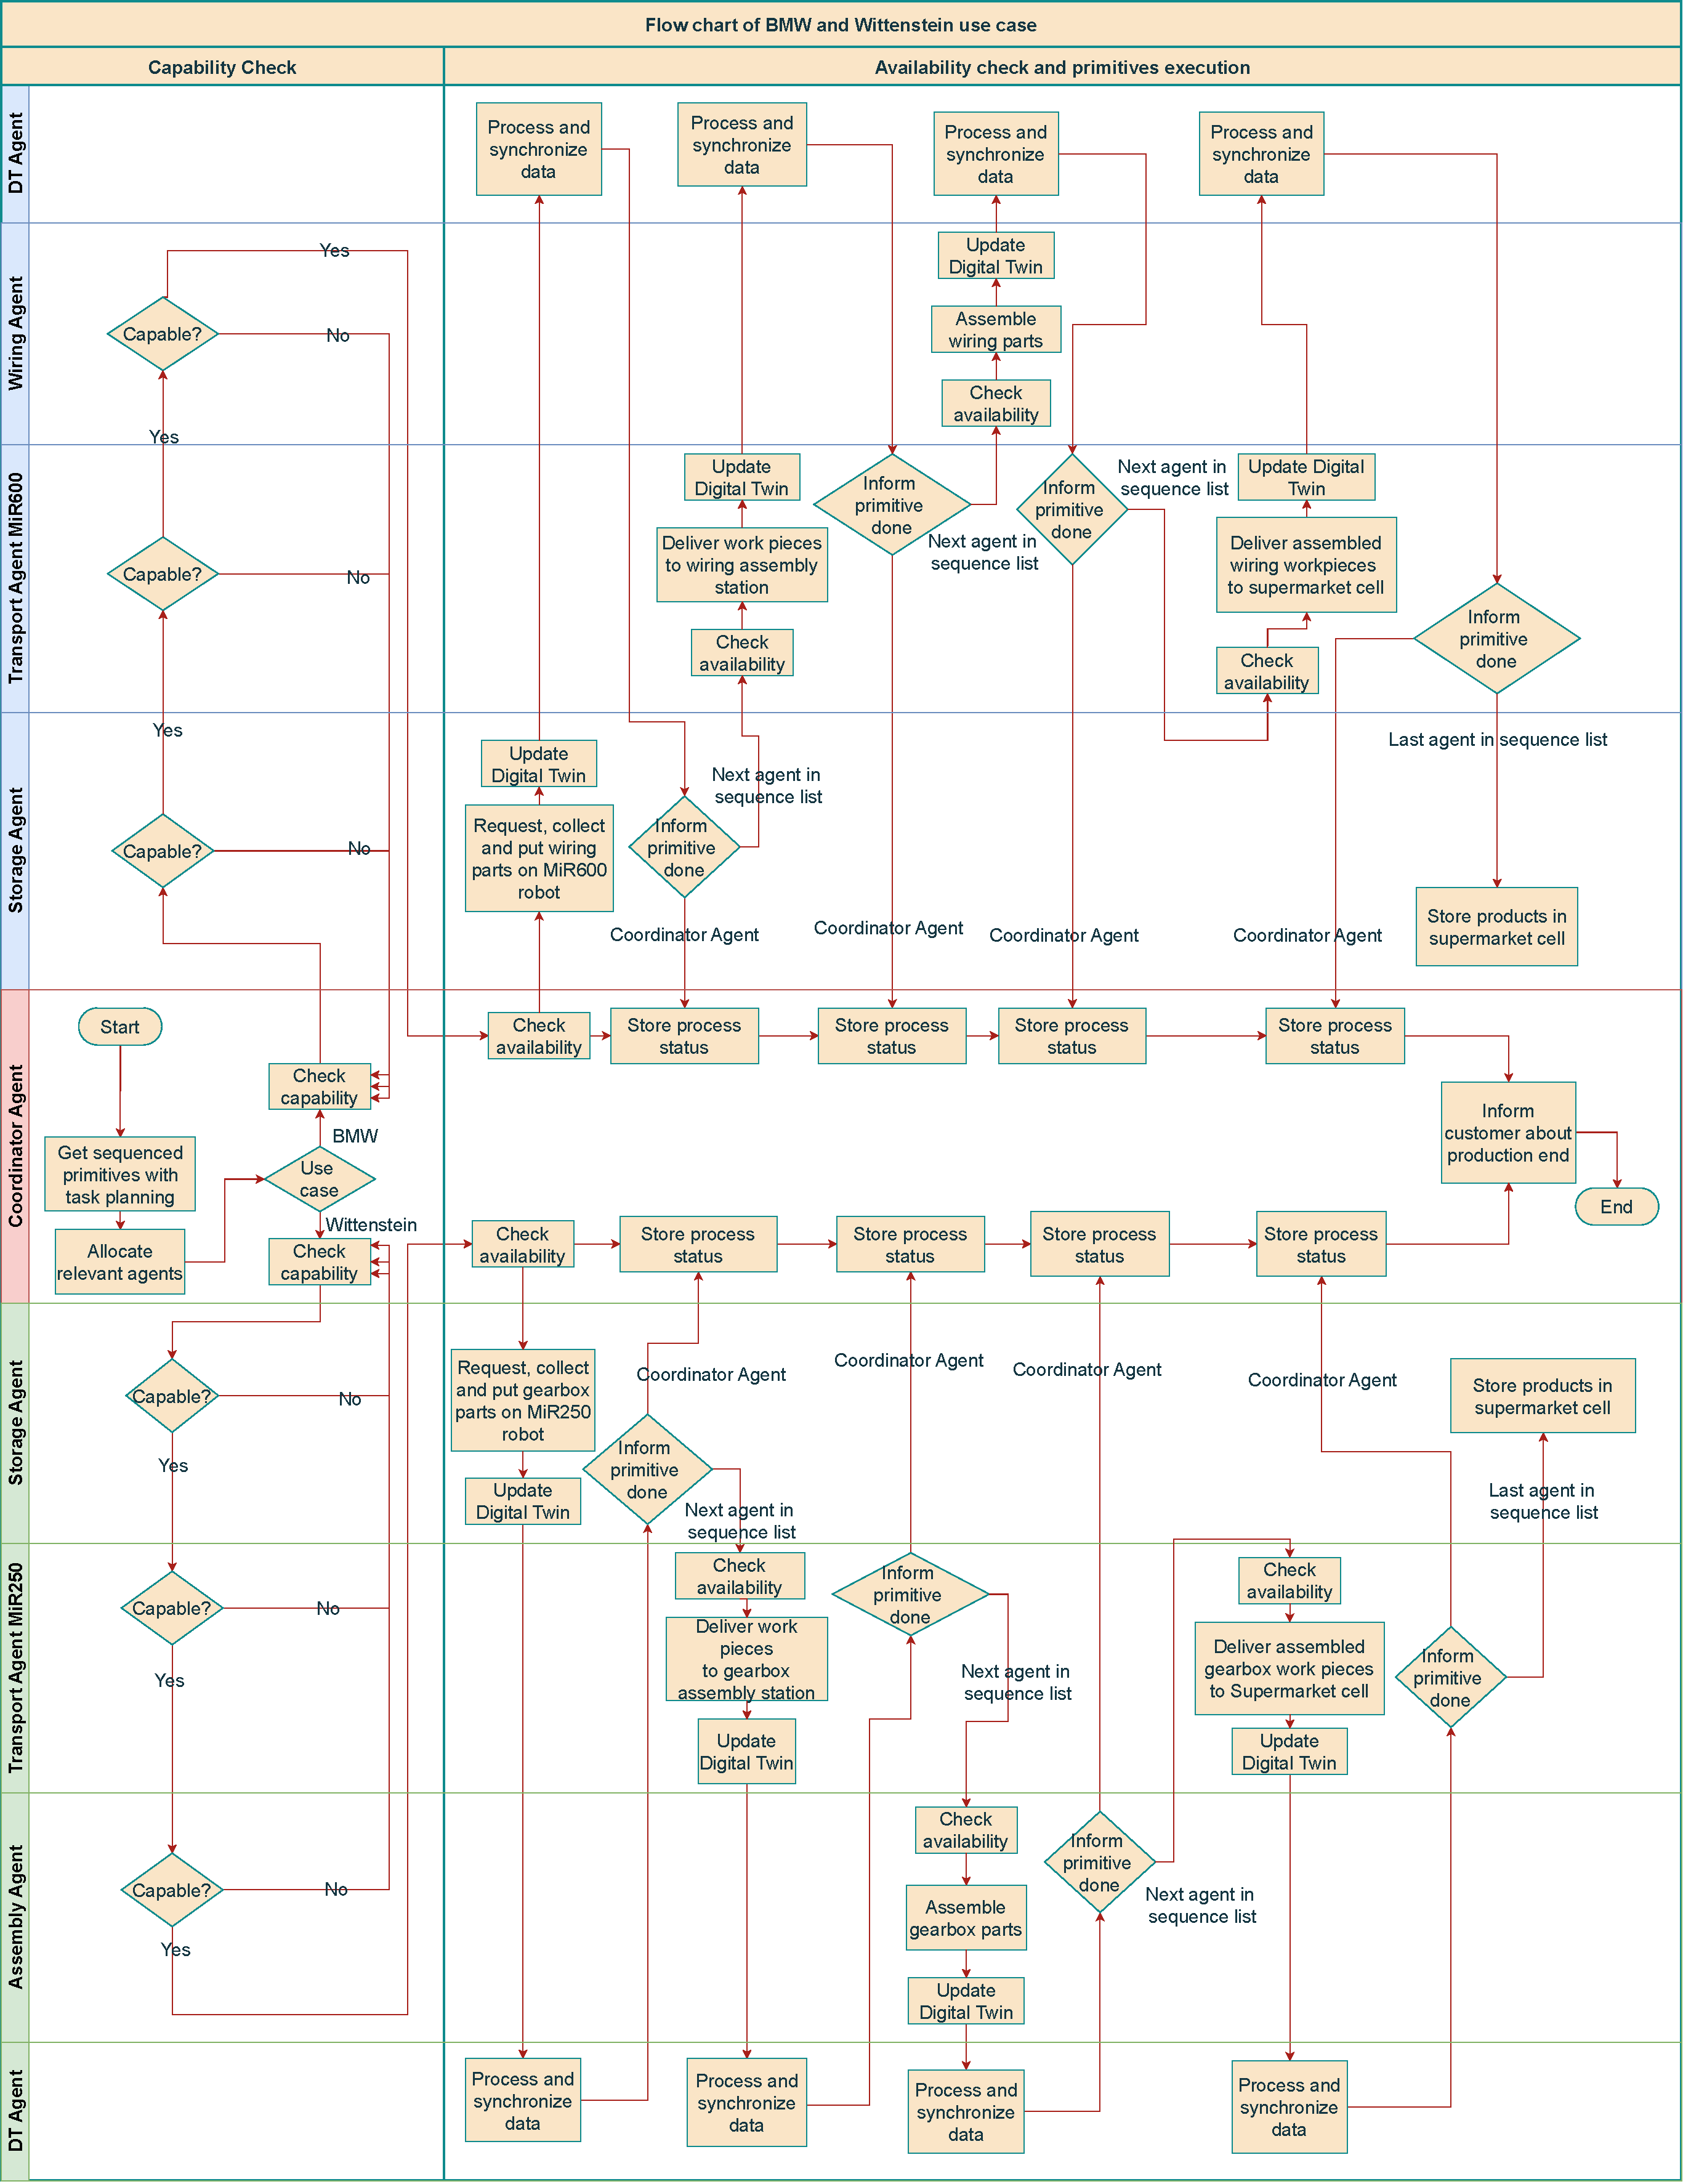
\includegraphics[width=\textwidth]{figures/tests/usecase/Usecase_flow.pdf}\hfill 
    \caption{Flowchart of BMW and Wittenstein use case of the \gls{mas} architecture. 
    Blue containers: BMW use case, allocated agents are Storge agent, 
    Transport agent MiR600, Wiring agent and Digital Twin agent respectively. 
    Green Containers: Wittenstein use case, allocated agents are Storage agent, 
    Transport agent MiR250, Assembly agent and Digital Twin agent respectively. 
    Red container: \gls{cda} for both usecases.} 
    \label{fig: Flowchart-usecase}
\end{figure}



For both BMW and Wittenstein use cases, the primitives with the associated agents and execution sequence are 
predefined. Although the program was designed based on two use cases, 
only the timing behaviors of the BMW use case was tested based on their similarity. 
The tab.\ref{tab: mean-usecase-time} shows the average \gls{rtt} and WebSocket 
data transmission time of BMW use case. The test was conducted a total of 100 times, 
but the number of messages 
each agent sent to the others during the test varied greatly. 
Due to the uneven amount of test data, 
the test results 
and average values can only be used as a reference to understand the data 
transmission process in actual production. A more detailed data ditribution of each 
message is presented as violin plot in fig.\ref{fig: violin-CDA-T600}. Together 
with the rest of the test results with other agents 
(see \ref{chap: append-UC} fig.\ref{fig: violin-CDA-ST} to \ref{fig: violin-T600-WI}), 
it can be concluded that 
the message transport in the system meets the real-time requirements, with the 
largest messge size of 636 Bytes in maximal 10ms and the smallest in about 0.2ms. 


\begin{table}[htbp]
    \small
    \centering
    \caption{Average delays between agents with different string message length and 
    different amount of messages.}
    \label{tab: mean-usecase-time}
    \begin{tabular}{|m{0.13\textwidth}|m{0.17\textwidth}|m{0.17\textwidth}|m{0.17\textwidth}|m{0.17\textwidth}|}
    \hline
    \multicolumn{5}{|c|}{\textbf{Average delays between agents (RTT/Transmission time)}}                                                            \\ \hline
    \textbf{}                         & \textbf{Coordinator Agent}             & \textbf{Storage Agent}        & \textbf{Transport Agent MiR600}    & \textbf{Wiring Agent}\\ \hline
    \textbf{Coordinator Agent}      & None                  & 1.029355ms /0.820172ms & 1.067170ms /0.849335ms  & 1.032151ms /0.817049ms \\ \hline
    \textbf{Storage Agent}          & 0.998253ms /0.794590ms & None                  & 1.427890ms /1.158142ms  & None                  \\ \hline
    \textbf{Transport Agent MiR600} & 1.055389ms /0.840291ms & 1.422970ms /1.150696ms & None                   & 1.668750ms /1.344250ms \\ \hline
    \textbf{Wiring Agent}           & 0.988012ms /0.783014ms & None                  & 1.654000ms /1.361000ms  & None                  \\ \hline
    \end{tabular}
\end{table}


\begin{figure}[htb]
    \centering
    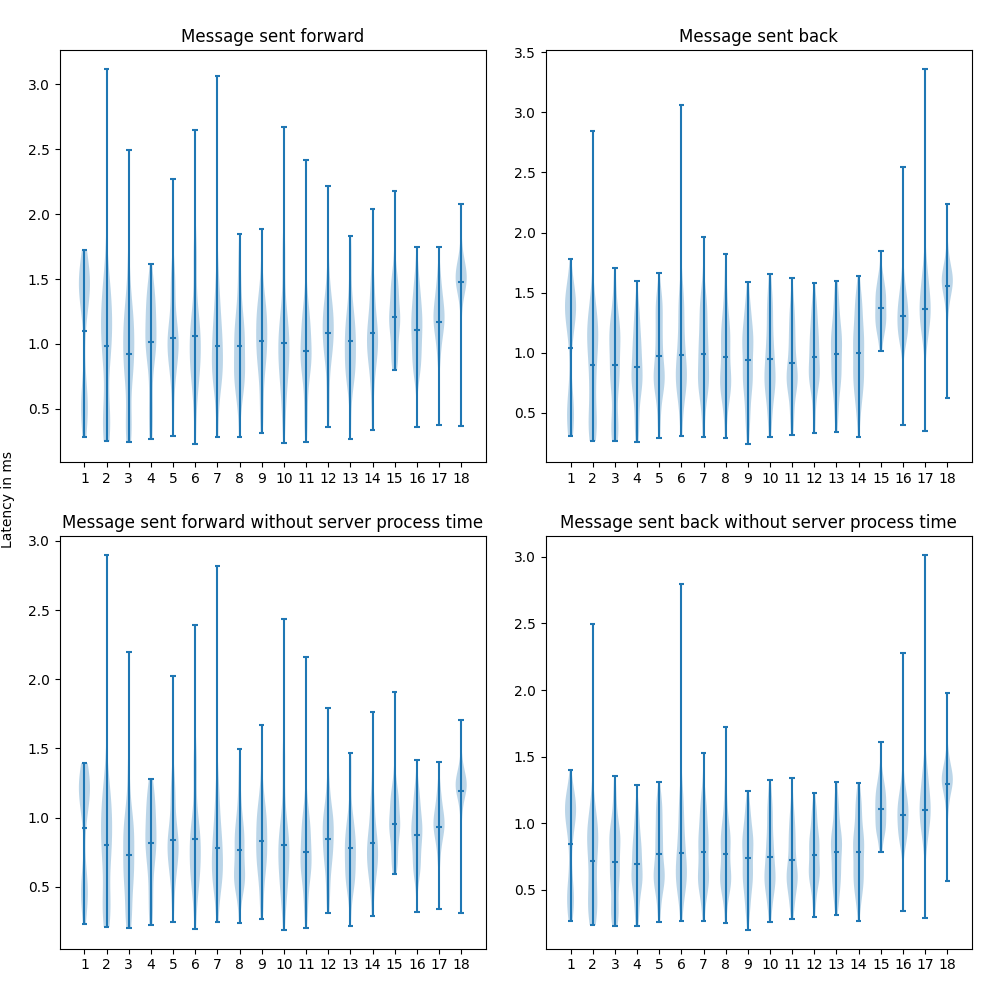
\includegraphics[width=\textwidth]{figures/tests/usecase/violin_CoordinatorAgent_to_TransportAgent_MiR600.png}\hfill 
    \caption{Test to measure \gls{rtt} and transmission time between \gls{cda} and 
    TransportAgent\_MiR600 for 100 times. The number in x-axis respresents the 
    corresonding messages. \protect\ref{firstfootnote}}
    \label{fig: violin-CDA-T600}
\end{figure}

%addtional for footnote in caption
\footnotetext[1]{\label{firstfootnote}https://github.com/XuezhouHou/Websocket\_MAS/new\_MAS/output/plots/table4UCBMW.xlsx}



\section{External}\label{chap: Result-External}
As for the delay measurement of the external \gls{dta} system, tests for the 
upload and download are done separately, with different packet sizes as tuning 
parameters. 


\subsection{Test results of data transmission time in \gls{tcp} sockets between robots and \gls{dta} 
in different packet lengths} \label{chap: Result-RCP-DTA}

To better measure the influence of different packet lengths on transmission time from 
a \gls{rcp} to \gls{dta} utilizing 
\gls{tcp} sockets, 
the packet length of JointGripper (joint and gripper of the robot arm) position values should 
be larger than that of the Elbow (elbow of the robot arm), they are 151 and 80 Bytes respectively. 
As depicted in 
fig.\ref{fig: SR-JointGripper-Elbow}, the mean transmission time of JointGripper is larger 
than Elbow, which verifies that larger files take longer to transfer. The cumulative delays of 
both data lengths also show a linear growth relationship 
in the upper graph, which means, there are no major fluctuations or irregularities 
in transmission speeds or times for the packets in \gls{tcp} sockets. 


\begin{figure}[htb]
    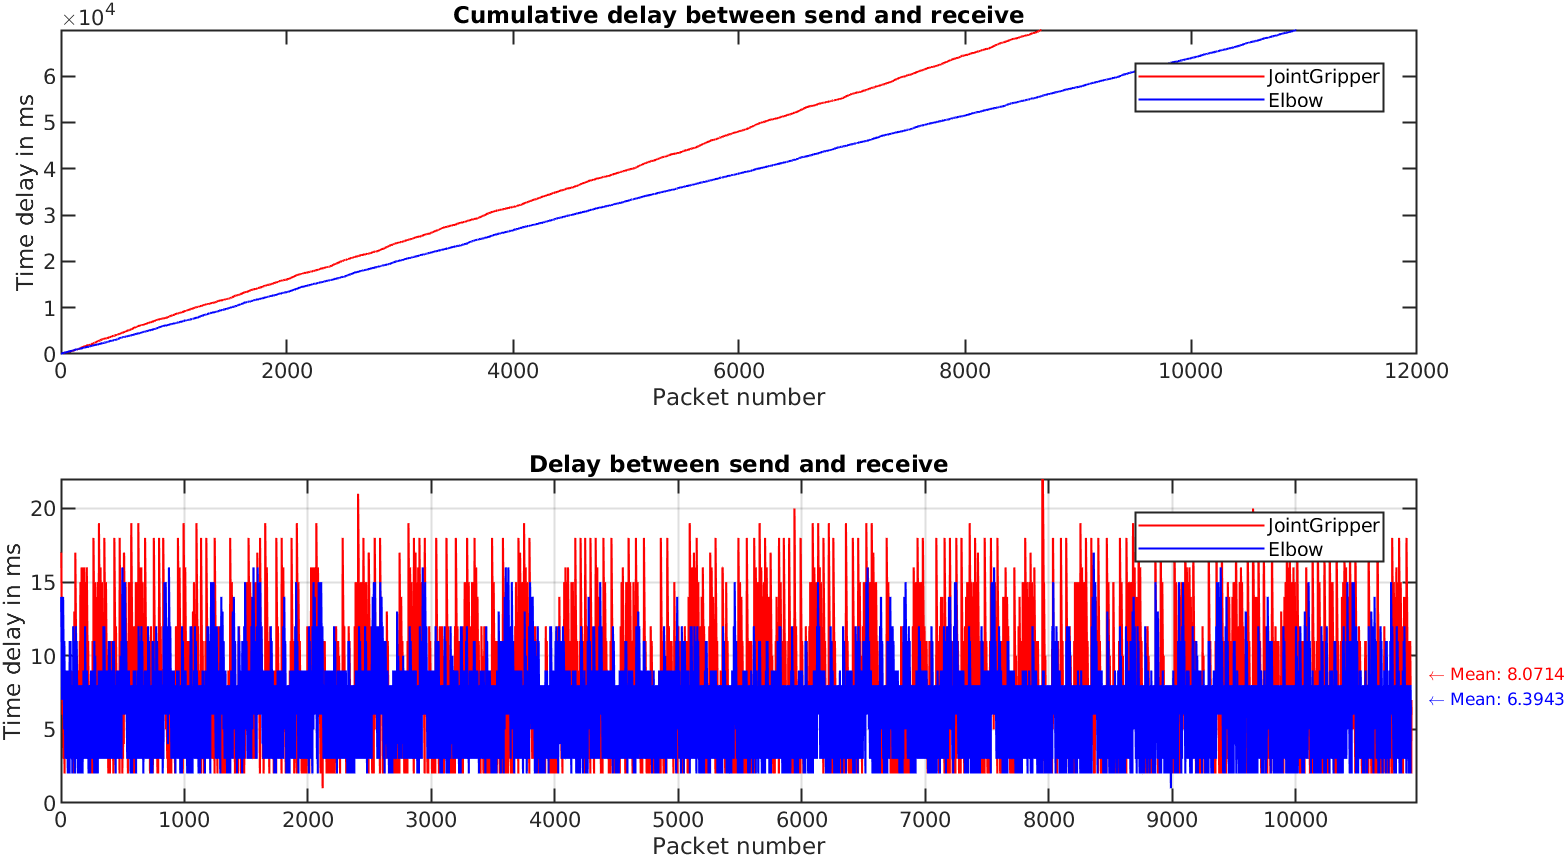
\includegraphics[width=\textwidth]{figures/tests/DT/Delay_SendReceive_JointGripper_Elbow.png}
    \centering
    \caption{Tests for different packet sizes w.r.t data transmission time between robots 
    and \gls{dta}. \label{fig: SR-JointGripper-Elbow}}
\end{figure}

Since each packet only takes a few milliseconds to be transported, the real time requirement 
for production processes is again fullfilled. 



\subsection{Test results of data transmission time in \gls{tcp} sockets between \gls{dta} 
and \gls{ms} Azure Digital Twin Cloud in different packet lengths} \label{chap: Result-DTA-DT}

However, in the program, the biggest variance 
on the total data transmission time is the \gls{rtt} from local devices to the global digital 
twin. In addtion to the \gls{rtt}, the data upload and download time is also measured 
separately, which has an opposite result as those from the other research\cite{cainelli_performance_2023}. 
In the paper, the resulting uplink data transmission time is larger than the downlink data transmission 
time. The difference between both tests is, the research team from Magdeburg 
measured delay with logical links from a 5G standalone network and the industrial 5G devices, 
whereas our test was based on data update times in the cloud. The latency 
between data upload and update reflects the actual digital twin data update 
patterns which includes additional process time in the cloud. Therefore we can 
infer that the increased latency of data upload may be caused by the internal 
Azure Digital Twin Model API for data update 
(unclosed issue in \gls{ms} Q\&A\footnote{https://learn.microsoft.com/en-us/answers/questions/1328803/experiencing-slow-load-times-on-azure-digital-twin}).
    

It is worth mentioning that the data upload time from JointGripper and Elbow 
has little to no difference, since the upload mechanism of Azure Digital Twin is limited 
by sending twin values one after one. There is no such function to update more than 
one twin simultaneously. In order to differentiate the upload speed, the patch size 
of the to be updated twin values should vary. The fig.\ref{fig: UD-cycle-JointGripper} 
again shows the cumulative delays with the same conclusion as in 
fig.\ref{fig: SR-JointGripper-Elbow} and mean \gls{rtt} is slightly lower than 
100ms, which is still under the real time requirements. As the packet for upload 
and download will be routed to the cloud, which not only goes through 
the internal 5G network but also the internet externally, which results in a much 
higher latency. Compared with the tests results from \cite{cainelli_performance_2023}, 
the internal twin update mechanisms can be optimized to further reduce the data 
upload and download \gls{rtt}. 


\begin{figure}[htb]
    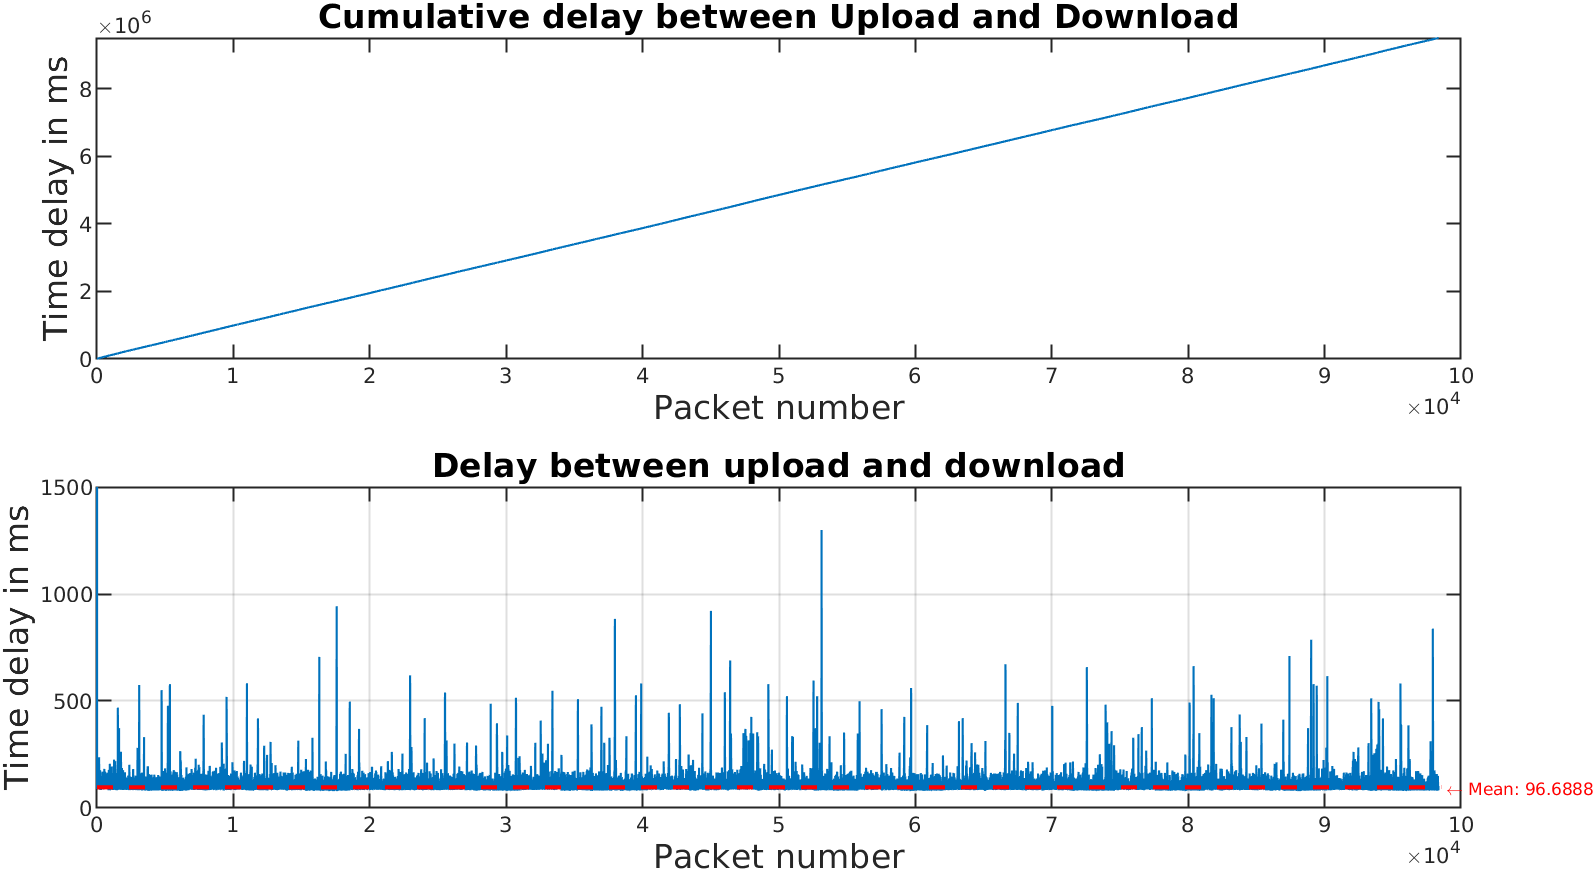
\includegraphics[width=\textwidth]{figures/tests/DT/Delay_UploadDownloadCycleTime_JointGripper.png}
    \centering
    \caption{Tests for \gls{rtt} of data upload and download for JointGripper. \label{fig: UD-cycle-JointGripper}}
\end{figure}

As mentioned, the data upload time is larger than the download time as depicted in 
fig.\ref{fig: UD-sep-JointGripper}. The upload time of JointGripper values is 
under 30ms while the download time results in about 70ms. Under the same conditions, 
the differences of both values for Elbow are negligible with 
only 1-2ms difference(see \ref{chap: append-DTagent} fig.\ref{fig: UD-cycle-Elbow} and 
\ref{fig: UD-sep-Elbow}), due to the one after one twin upload mechanism. 




\begin{figure}[htb]
    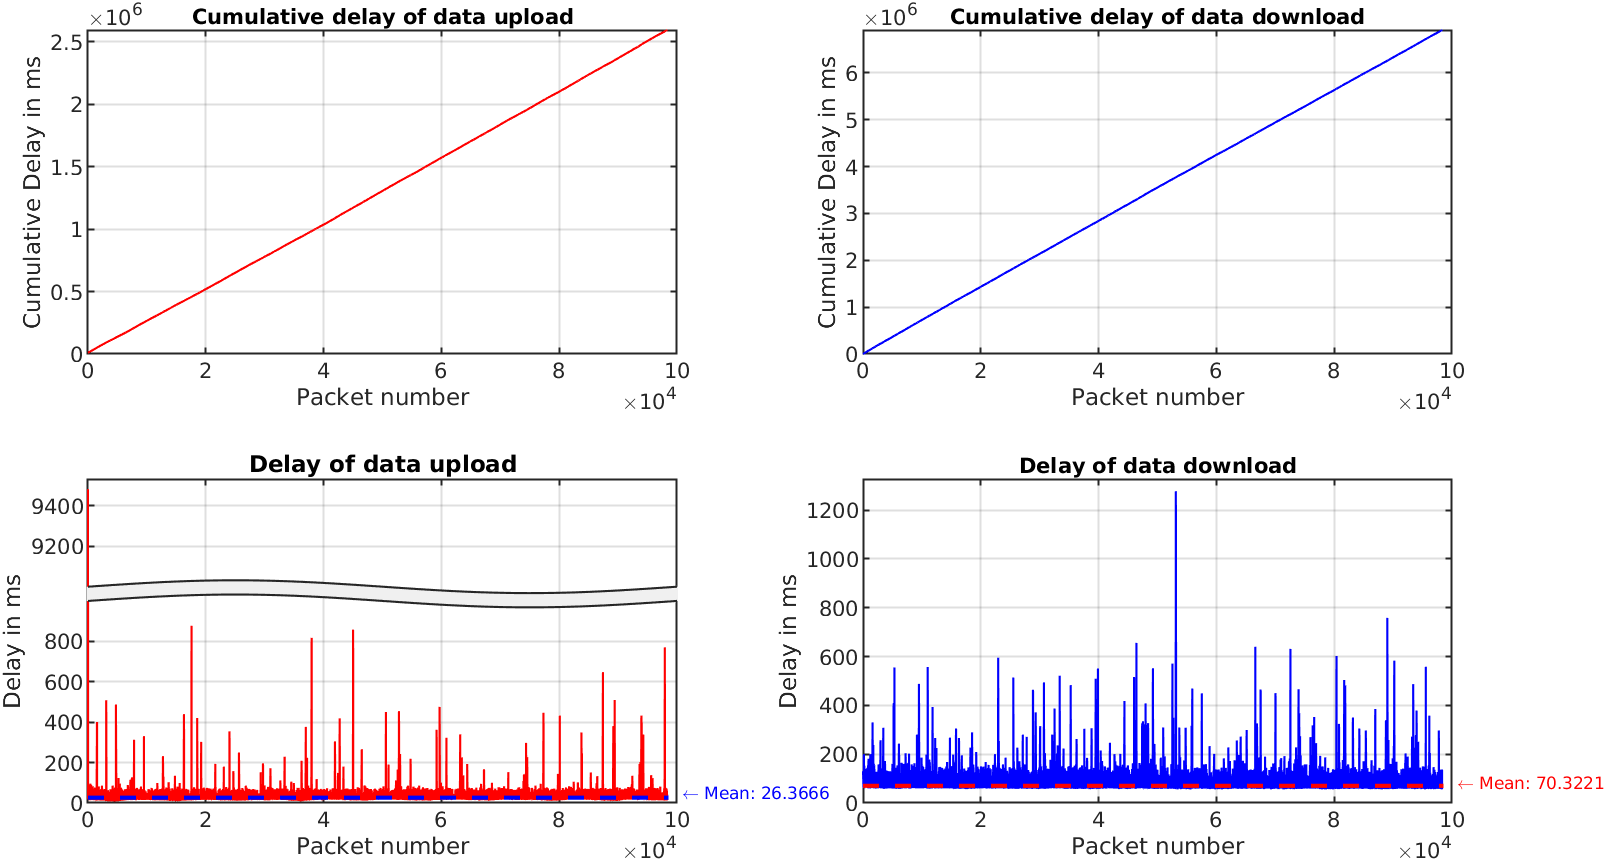
\includegraphics[width=\textwidth]{figures/tests/DT/Delay_UploadDownload_JointGripper.png}
    \centering
    \caption{Tests for delays between \gls{dta} and digital twin update of JointGripper, 
    and delays for twin value download. \label{fig: UD-sep-JointGripper}}
\end{figure}


To differentiate the upload speed based on packet size, two patches with 
different sizes are introduced. Ideally, the small data patch with a size of 
49 Bytes should induce a higher transmission speed than the large one with 
554 Bytes, but the reality is quite different. The test results of all the 
delay measurement for both patch sizes are presented as a violin plot in 
fig.\ref{fig: UD-violin-patchsize}. As expected, the upload time of large 
patches is less than small patches, while the result of download time is the 
opposite. This results to a almost identical total \gls{rtt} of both. 
The reasons can be, that each test is done at different time, which results in 
a fluctuation related to the network traffic, cloud service loads, amount of 
end users under the same 5G network and many more, which influence the data transmission 
time even more than the patch sizes.

\begin{figure}[htb]
    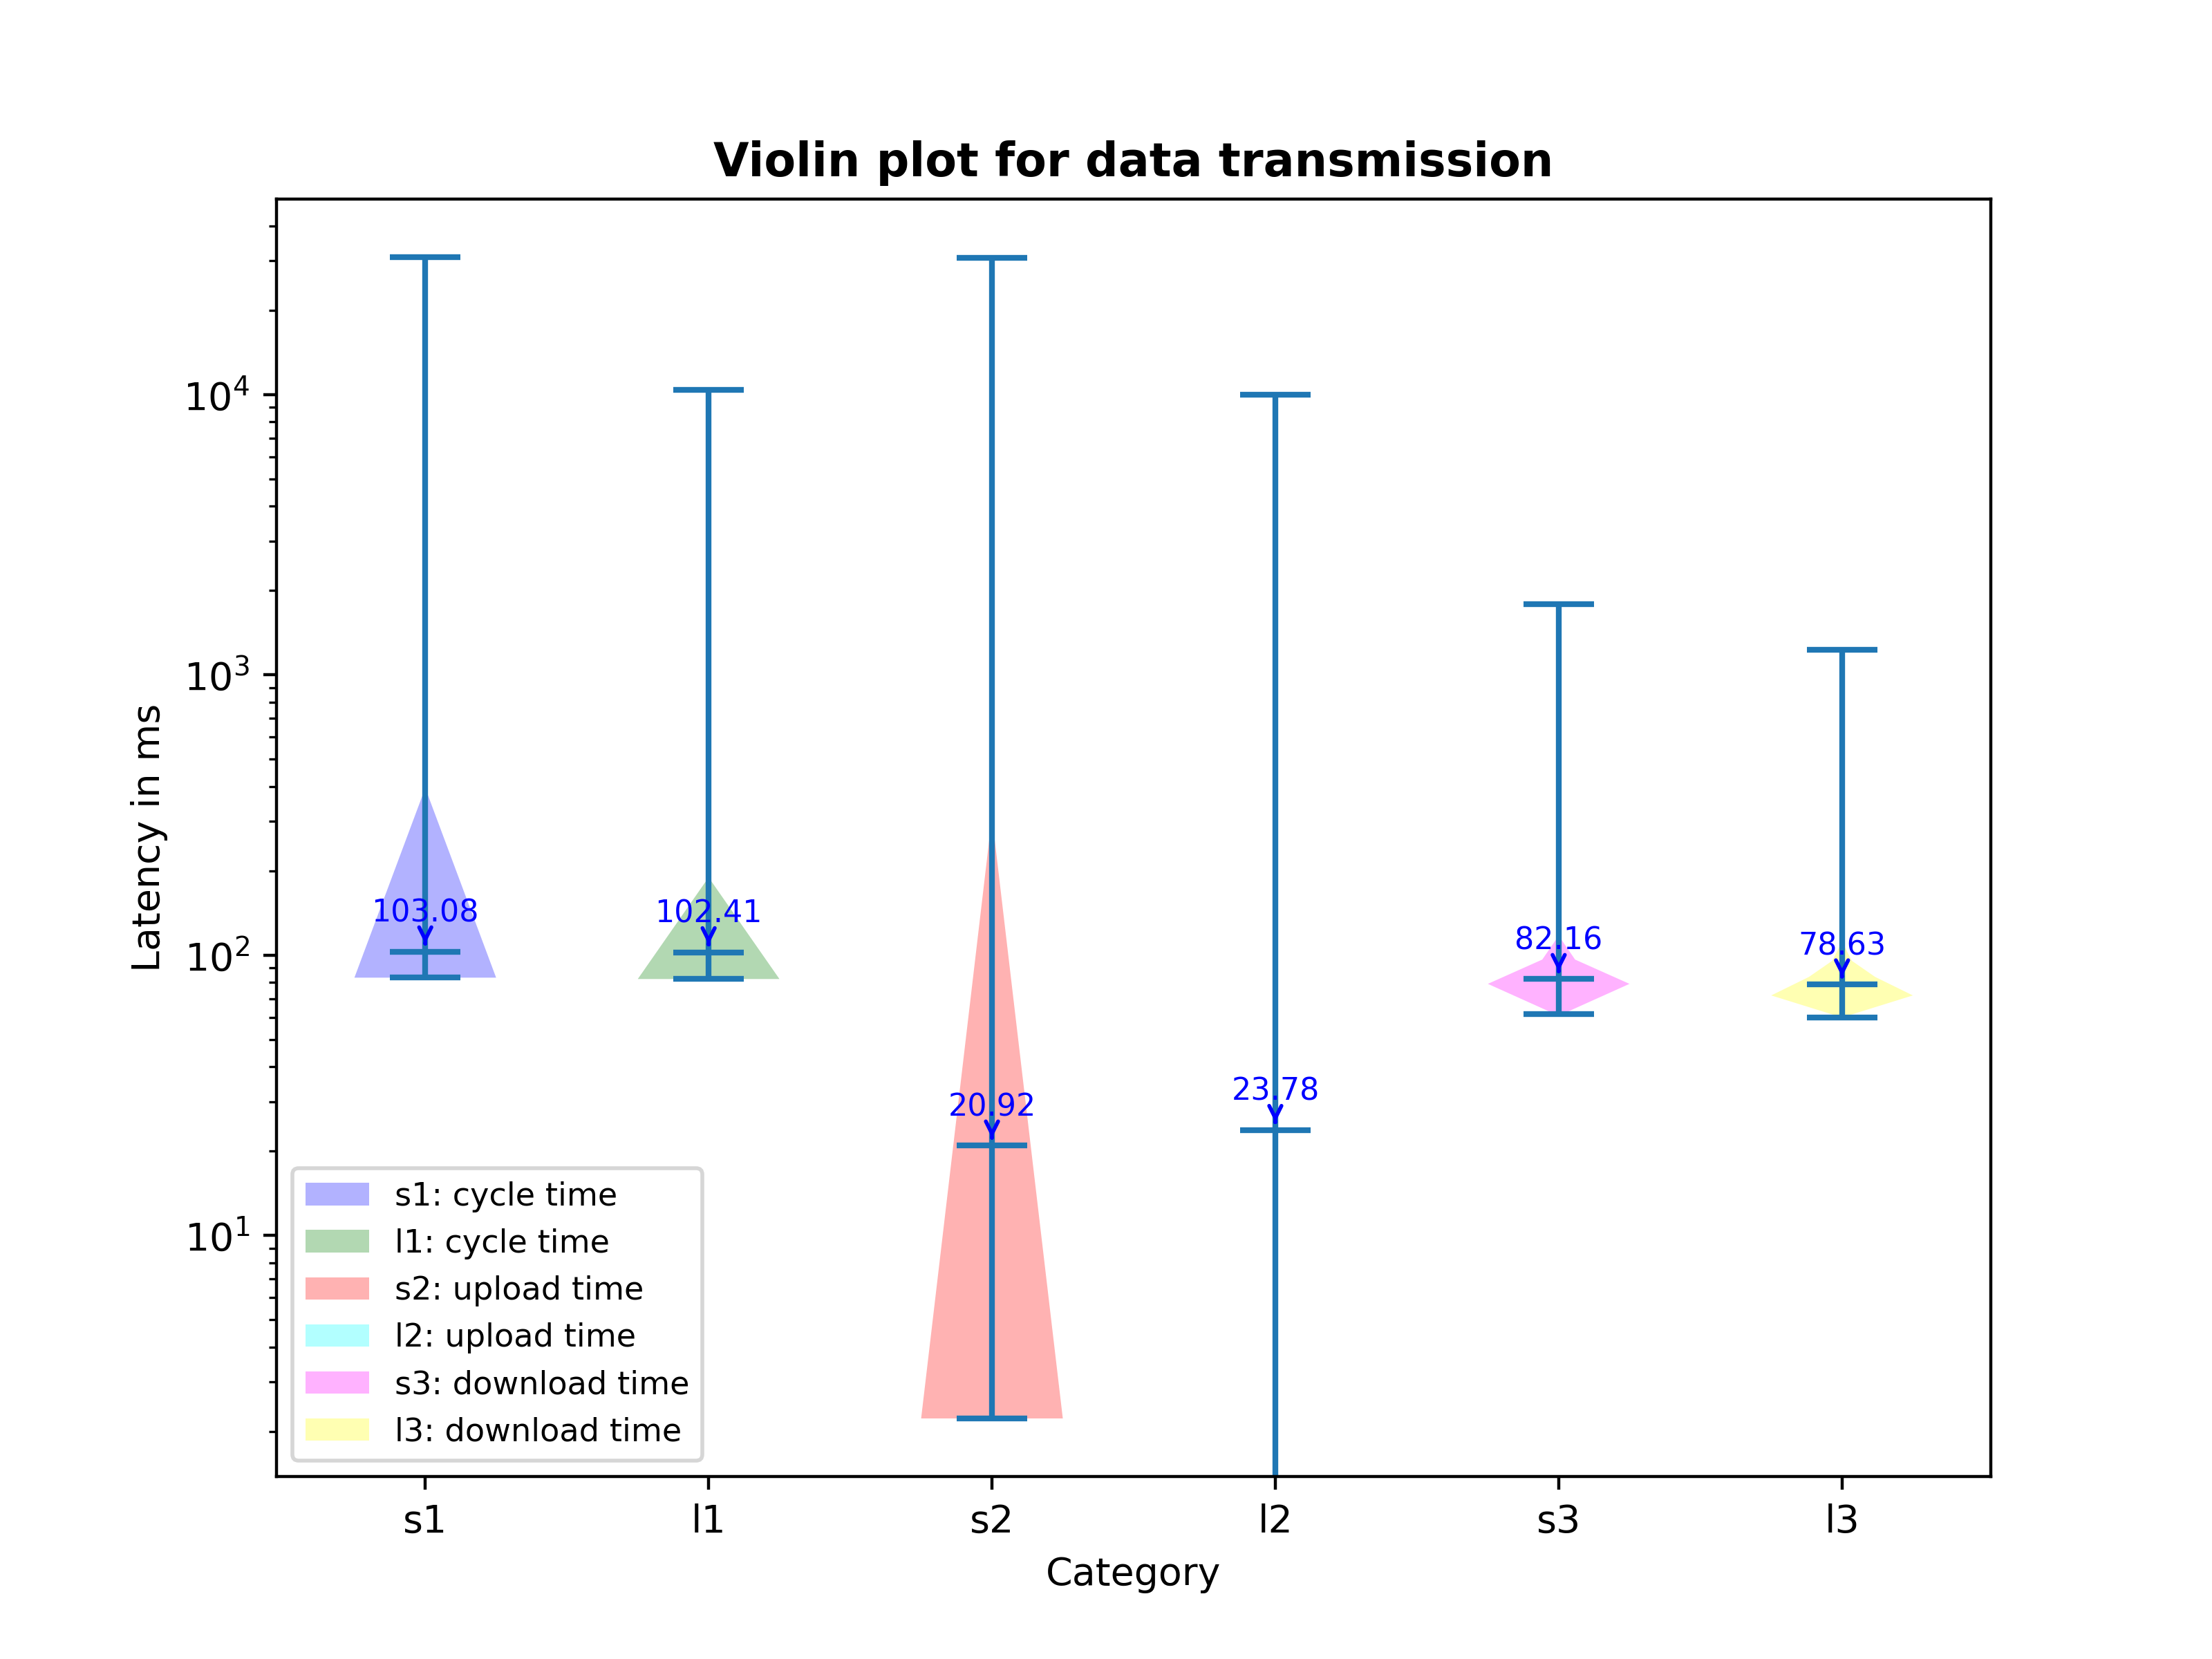
\includegraphics[width=\textwidth]{figures/tests/DT/violin_patch_size.png}
    \centering
    \caption{Tests for \gls{rtt}, delays between \gls{dta} and digital twin 
    update of JointGripper, and delays of twin value download for 
    two different patch sizes. In the graph, s represents small patches 
    and l for large patches.\label{fig: UD-violin-patchsize}}
\end{figure}

In genral, the data upload and download time between \gls{dta} and the cloud 
is much higher than the field 
level data transmission time under \gls{tcp} sockets. A fig.\ref{fig: SR-U-D-violin} shows 
the variance and mean of those in a violin plot for a more intuitive observation. 
Compared to the violin plot in fig.\ref{fig: UD-violin-patchsize}, the send and receive 
processes always show a symmetric triangular shape, suggesting a limited sample size. 
Considering the non-symmetric triangular shape of 
the uploading and downloading processes, 
this is likely be attributed to the data points with a predominance at the lower extremum, 
and the minimal presence at the upper extremum.
\begin{figure}[htb]
    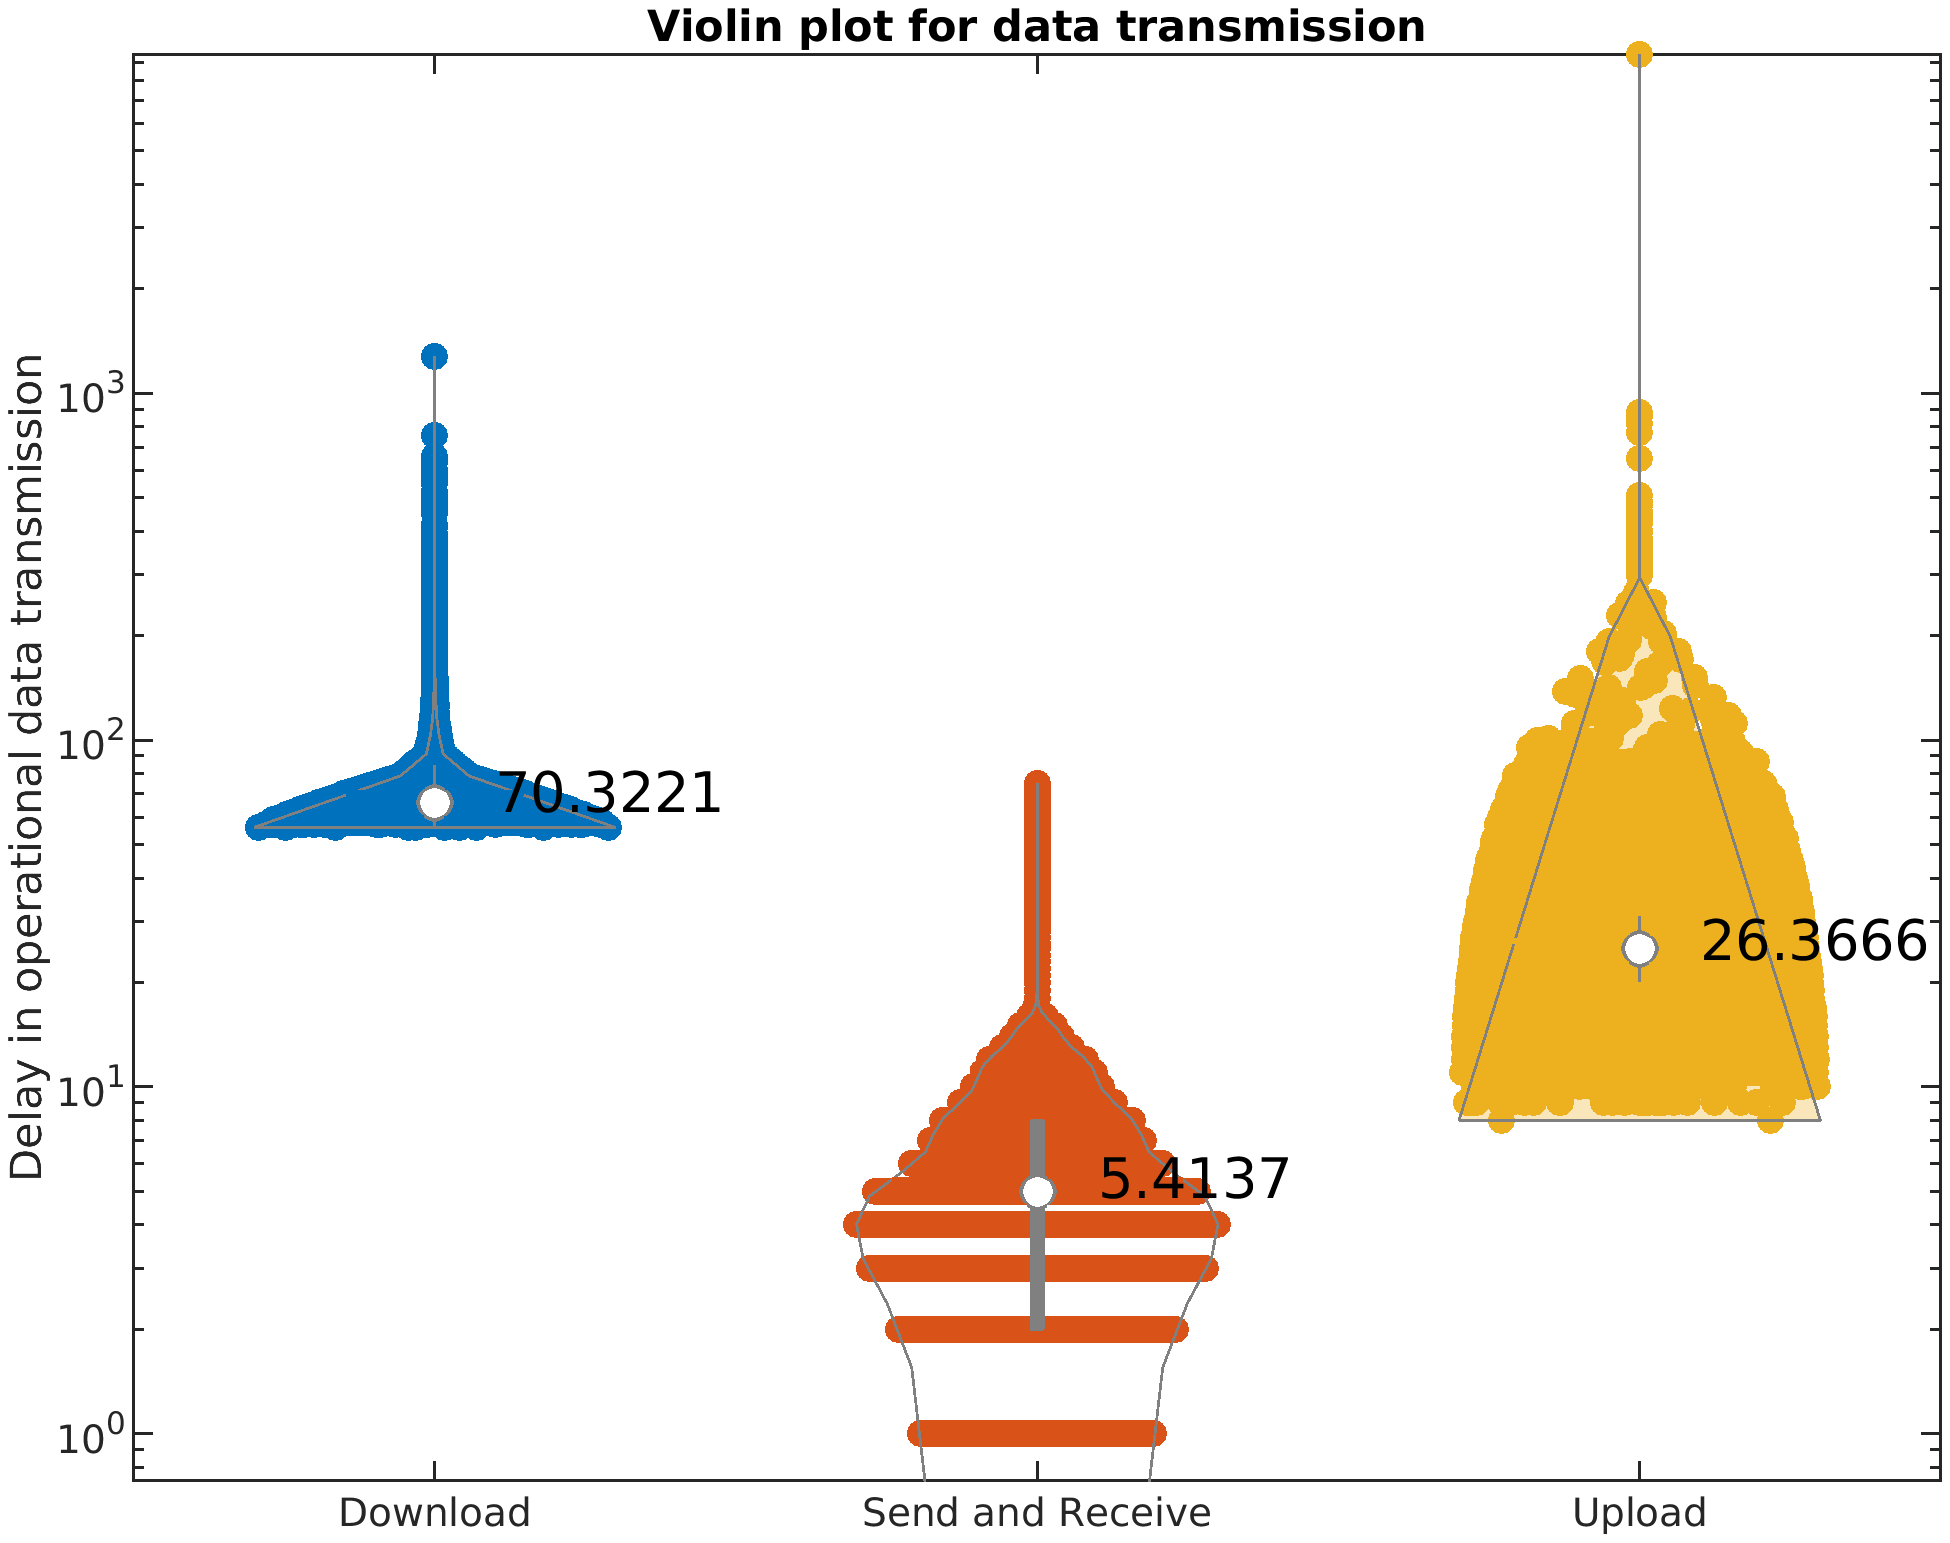
\includegraphics[width=\textwidth]{figures/tests/DT/log_violin_Plot_3cat.png}
    \centering
    \caption{Tests for data transmission time from robot to \gls{dta}, 
    delays between \gls{dta} and digital twin 
    update of JointGripper, and delays for twin value download.\label{fig: SR-U-D-violin}} 
\end{figure}

%
\chapter{Conclusion and outlook}

In this article, we emphasize that in modern factories, in order to handle 
multi-tasking problems, it is essential to introduce the concept of system 
decentralization. Considered a modern and effective solution to system 
decentralization, \gls{mas} is incredibly functional for domain-specific 
applications. By applying \gls{mas} to a traditional master-slave\cite{egger_deployment-friendly_2020} 
pattern, we now obtained a system that is mainly scheduled and coordinated 
by \gls{cda} who receives the customer requirements and break those down to agent 
executable primitives, supplemented by other intelligent \gls{ras} that proceed 
with those primitives, to enable the 
autonomous decision-making and planning in each agent. Distinct from a 
general \gls{mas}, we extended its domain to \gls{iot} by 
introducing an additional \gls{dta} to bridge the gap between physical 
entities and \gls{dt}. On top of the existing Azure \gls{dt} architecture, we 
added an Azure Event Hub and Azure Data Explorer inside the \gls{dta} data 
flow cycle to store and analyze the data. 


To represent the systems, we designed two programs for both local 
\gls{mas} and \gls{dta}, with the name Websocket\_MAS and DTAgent 
(along with a \gls{rcp}). Although both can transfer data, the 
specific content required for production processes differs. For 
example, local \gls{mas} transmits commands for the agent's decision-making 
and planning, and \gls{dta} is responsible for the robot's raw data processing 
and routing between local devices and global \gls{dt}. Due to its high complexity 
of communication mechanism, local \gls{mas} is designed based on the application 
layer protocol WebSocket, which is exceptionally suitable for real-time required, 
bi-directional, and full-duplex agent-based communications. 
In comparison, the data transport in \gls{dta} is one-directional, which allows 
a simple, more-to-one server-client communication based on the transport layer 
protocol \gls{tcp}. The choice of \gls{tcp} minimizes the packet header and 
guarantees a stable and secure data transport through the internet. In fact, 
all the agents are connected by a 5G wireless network, which makes it possible 
to capture, compare, and analyze the delays between each other. As we all know, 
many factors influence network delays: the transmission medium (e.g., wireless), 
the distance between two transport entities, network traffic, bandwidth, 
throughput, and so forth. To ensure that the collaborative robot operation 
system meets real-time requirements, it is crucial to minimize network delays. 



In this article, we conducted many tests to analyze the network delays 
for both systems. Those tests for \gls{mas} communications can be roughly 
divided into three types: performance tests for an increasing number of servers, 
clients, and message lengths in different types, including worst-case scenarios, 
message prioritization mechanism in server design for critical messages 
(e.g., emergent stop, important task prioritization), and a use case specific 
delay measurement to simulate real-world production process. Respecting \gls{dta}, 
the tests are more straightforward. We first measured the transmission delays of 
different robot states from \gls{rcp} to \gls{dta}, and then we performed tests 
for data upload and download between \gls{dta} and Azure \gls{dt}. Based on the 
results from \cite{cainelli_performance_2023} for uplink and downlink delay measurement under a 5G 
network, this results in a more significant delay by the former and less by the 
latter. In our test, we managed to separate the data upload and download \gls{owd} 
delays from the total cycle time by extracting the twin update time in 
Azure \gls{dt}. Our results show an opposite upload and download \gls{owd}, 
possibly due to a different network or cloud setup. Since many influencing 
factors exist, we can hardly analyze the network delays simply from the values. 



Therefore, we inherited the model-driven approach from the automation industry. 
There are already extended graphical notations based on \gls{dsl} that exist 
for analyzing the timing properties for both software and hardware under soft 
and hard real-time requirements\cite{hujo_toward_2022} and the modularization 
approaches for robot-like systems\cite{volpert_supporting_nodate}. Based on these 
considerations, we designed a graphical model to describe the timing properties 
and requirements for agent-based communication and robot control systems. 
In our model, the data follows a path to flow through the \gls{tcp/ip} layers 
after being processed in \gls{cpu} and again the same layers in the opposite 
direction to the receiver \gls{cpu} endpoint. Similarly, the robot control system 
also produces delays, which can be modularized as delays in technical processing, 
I/O module, and robot controller interface. 
Another modularization consideration is related to agent-based design architecture. 
According to the Wannagat's design pattern\cite{wannagat_agent_nodate}\cite{wannagat_entwicklung_2010}, instead of the delays, the 
functionalities for each agent can be categorized to five modules:  Planning 
module, control module, diagnosis module, knowledge base, and communication 
interface. In our \gls{mas} design, each module is interconnected to transfer 
states within an agent, where a series of tasks from each module is performed.


Our graphical notations provided insight into a more abstract and domain-specific 
modularization of timing properties for \gls{mas}, and decision-making and planning 
within each agent. 
Future work could be using the existing tools to measure or simulate delays for 
each module or developing a modeling tool for research purposes. And also, one improvement 
of the \gls{dta} system design could be introduing a real-time visualization platform 
for a more intuitive representation of the physical changes in robots' collaboration.%

%
% Appendix
% --------
\appendix%
\chapter{Appendices}\label{chap: append}
\section{Tests for string message priority}\label{chap: append-string-priority}
%
%priority tests
\begin{figure}[h]
    \centering
    \begin{subfigure}[b]{0.6\textwidth}
    \centering
    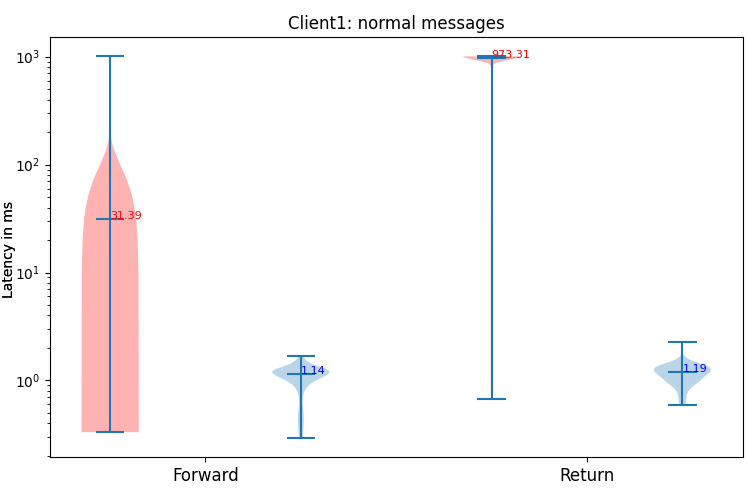
\includegraphics[width=\textwidth]{figures/appendix/priority_tests/log_violin_2clients_string_priority_client1.png}\hfill 
    \caption{} \label{fig: priority-2clients-string-1}
    \end{subfigure}
    \begin{subfigure}[b]{0.6\textwidth}
        \centering
        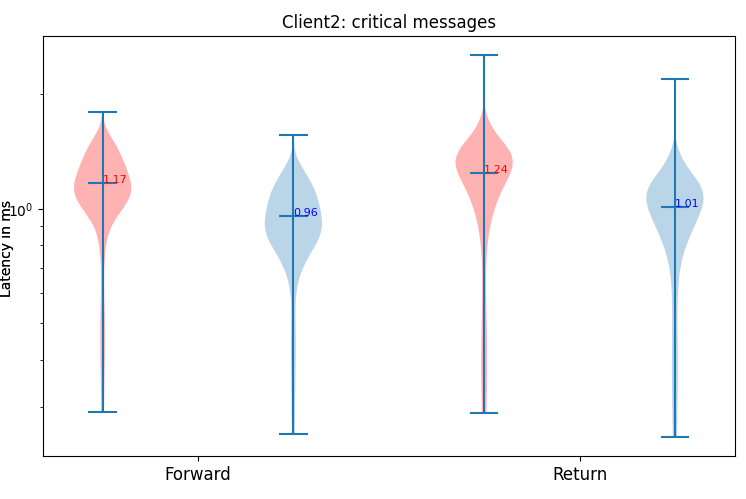
\includegraphics[width=\textwidth]{figures/appendix/priority_tests/log_violin_2clients_string_priority_client2.png}\hfill 
        \caption{} \label{fig: priority-2clients-string-2}
    \end{subfigure}
    
    
    \caption{Tests for timing properites of forward and return prioritized string messages between 2 clients 
    and clientR for 100 times. The blue violin represents the average data transmission time and the red violin 
    respresent mean \gls{owd}. (a) Client1 with normals messages, and (b) 
    with critical messages} \label{fig: priority-2clients-string}
\end{figure}



\begin{sidewaysfigure}[p]
    \centering
    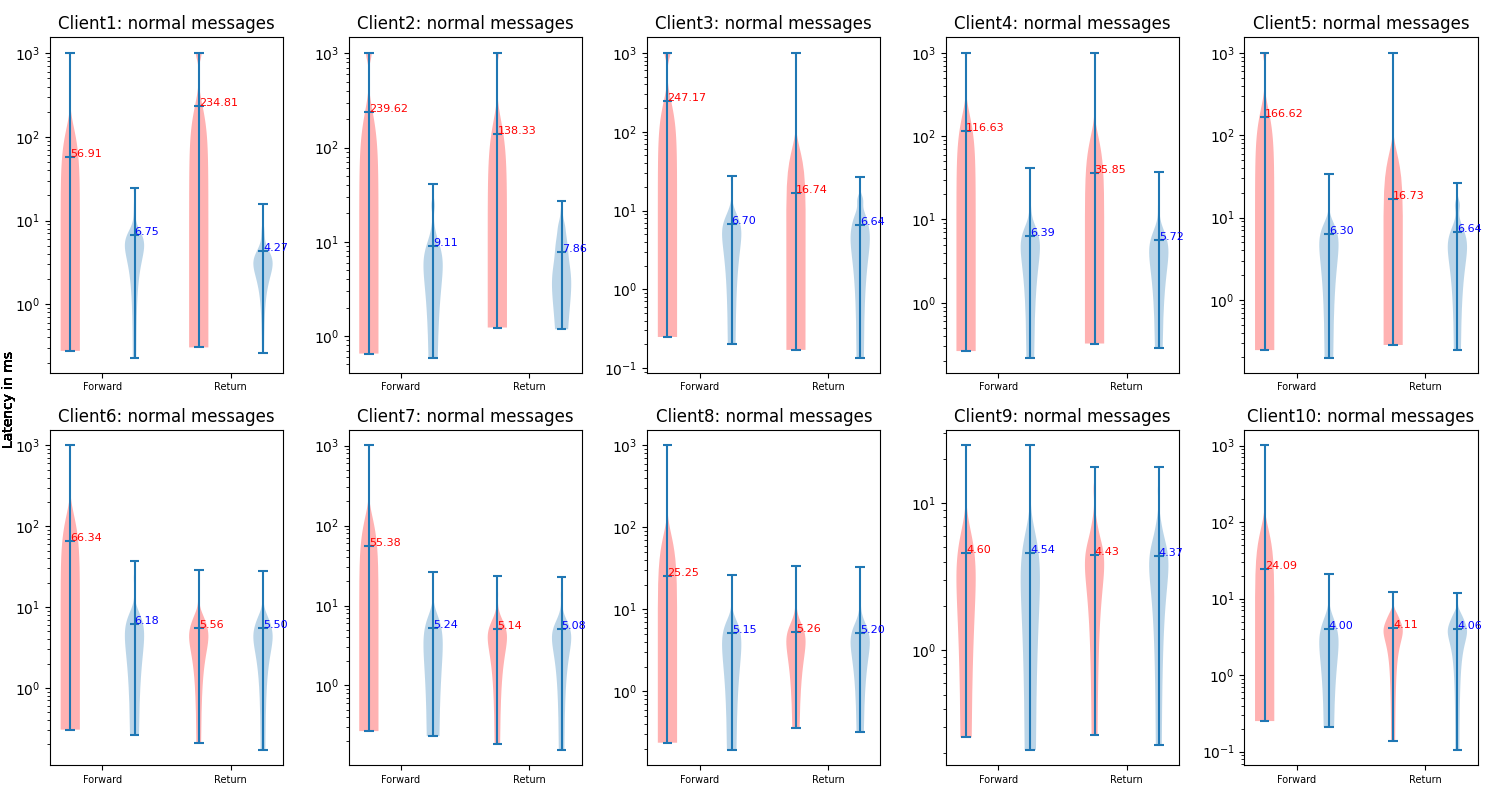
\includegraphics[width=\textheight]{figures/appendix/priority_tests/log_violin_50clients_string_figure_1.png}\hfill 
    \caption{Tests for timing properites of forward and return prioritized string messages between client1 to client10 
    with clientR for 100 times. The blue violin represents the average data transmission time and the red violin 
    respresent mean \gls{owd}.} \label{fig: priority-50clients-string-a}
\end{sidewaysfigure}

\begin{sidewaysfigure}[p]
    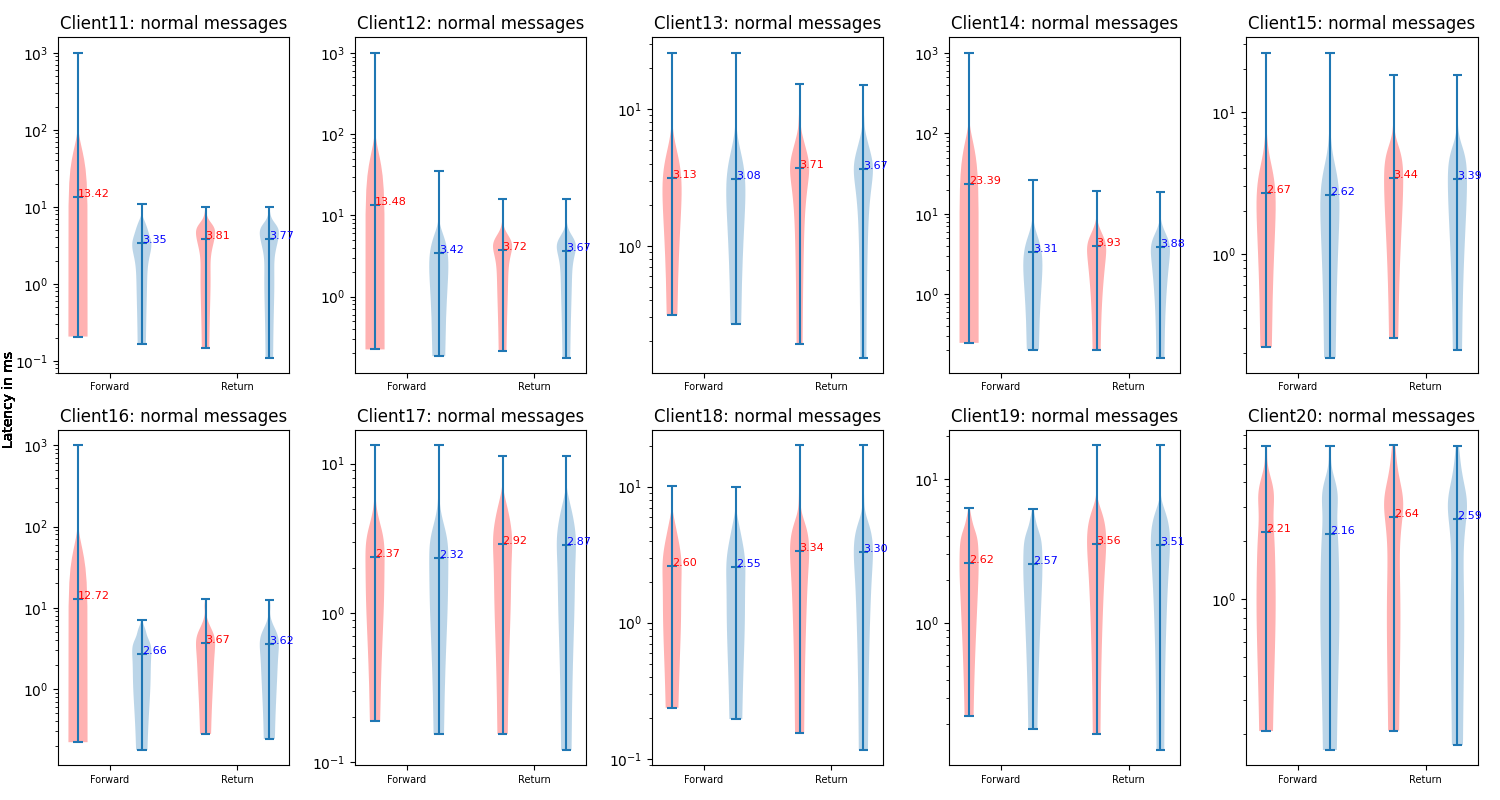
\includegraphics[width=\textheight]{figures/appendix/priority_tests/log_violin_50clients_string_figure_2.png}\hfill 
    \caption{Tests for timing properites of forward and return prioritized string messages between client11 to client20 
    with clientR for 100 times. The blue violin represents the average data transmission time and the red violin 
    respresent mean \gls{owd}.} \label{fig: priority-50clients-string-b}
\end{sidewaysfigure}

\begin{sidewaysfigure}[p]
    \includegraphics[width=\textheight]{figures/appendix/priority_tests/log_violin_50clients_string_figure_3.png}\hfill 
    \caption{Tests for timing properites of forward and return prioritized string messages between client21 to client30 
    with clientR for 100 times. The blue violin represents the average data transmission time and the red violin 
    respresent mean \gls{owd}.} \label{fig: priority-50clients-string-c}
\end{sidewaysfigure}

\begin{sidewaysfigure}[p]
    \includegraphics[width=\textheight]{figures/appendix/priority_tests/log_violin_50clients_string_figure_4.png}\hfill 
    \caption{Tests for timing properites of forward and return prioritized string messages between client31 to client40 
    with clientR for 100 times. The blue violin represents the average data transmission time and the red violin 
    respresent mean \gls{owd}.} \label{fig: priority-50clients-string-d}
\end{sidewaysfigure}

\begin{sidewaysfigure}[p]
    \includegraphics[width=\textheight]{figures/appendix/priority_tests/log_violin_50clients_string_figure_5.png}\hfill 
    \caption{Tests for timing properites of forward and return prioritized string messages between client41 to client50 
    with clientR for 100 times. The blue violin represents the average data transmission time and the red violin 
    respresent mean \gls{owd}.} \label{fig: priority-50clients-string-e}
\end{sidewaysfigure}


\newpage
\section{Tests image message priority}\label{chap: append-image-priority}


\begin{figure}[h]
    \centering
    \begin{subfigure}[b]{0.6\textwidth}
    \includegraphics[width=\textwidth]{figures/appendix/priority_tests/log_violin_2clients_image_priority_client1.png}\hfill 
    \caption{} \label{fig: priority-2clients-image-1}
    \end{subfigure}
    \begin{subfigure}[b]{0.6\textwidth}
        \includegraphics[width=\textwidth]{figures/appendix/priority_tests/log_violin_2clients_image_priority_client2.png}\hfill 
        \caption{} \label{fig: priority-2clients-image-2}
    \end{subfigure}
    
    
    \caption{Tests for timing properites of forward and return prioritized image messages between 2 clients 
    and clientR for 100 times. The blue violin represents the average data transmission time and the red violin 
    respresent mean \gls{owd}. (a) Client1 with normals messages, and (b) 
    with critical messages} \label{fig: priority-2clients-image}
\end{figure}



\begin{sidewaysfigure}[p]
    \centering
    \includegraphics[width=\textheight]{figures/appendix/priority_tests/log_violin_50clients_image_figure_1.png}\hfill 
    \caption{Tests for timing properites of forward and return prioritized image messages between client1 to client10 
    with clientR for 100 times. The blue violin represents the average data transmission time and the red violin 
    respresent mean \gls{owd}.} \label{fig: priority-50clients-image-a}
\end{sidewaysfigure}

\begin{sidewaysfigure}[p]
    \includegraphics[width=\textheight]{figures/appendix/priority_tests/log_violin_50clients_image_figure_2.png}\hfill 
    \caption{Tests for timing properites of forward and return prioritized image messages between client11 to client20 
    with clientR for 100 times. The blue violin represents the average data transmission time and the red violin 
    respresent mean \gls{owd}.} \label{fig: priority-50clients-image-b}
\end{sidewaysfigure}

\begin{sidewaysfigure}[p]
    \includegraphics[width=\textheight]{figures/appendix/priority_tests/log_violin_50clients_image_figure_3.png}\hfill 
    \caption{Tests for timing properites of forward and return prioritized image messages between client21 to client30 
    with clientR for 100 times. The blue violin represents the average data transmission time and the red violin 
    respresent mean \gls{owd}.} \label{fig: priority-50clients-image-c}
\end{sidewaysfigure}

\begin{sidewaysfigure}[p]
    \includegraphics[width=\textheight]{figures/appendix/priority_tests/log_violin_50clients_image_figure_4.png}\hfill 
    \caption{Tests for timing properites of forward and return prioritized image messages between client31 to client40 
    with clientR for 100 times. The blue violin represents the average data transmission time and the red violin 
    respresent mean \gls{owd}.} \label{fig: priority-50clients-image-d}
\end{sidewaysfigure}

\begin{sidewaysfigure}[p]
    \includegraphics[width=\textheight]{figures/appendix/priority_tests/log_violin_50clients_image_figure_5.png}\hfill 
    \caption{Tests for timing properites of forward and return prioritized image messages between client41 to client50 
    with clientR for 100 times. The blue violin represents the average data transmission time and the red violin 
    respresent mean \gls{owd}.} \label{fig: priority-50clients-image-e}
\end{sidewaysfigure}




%use cases
\newpage
\section{Tests for BMW use cases}\label{chap: append-UC}

\begin{figure}[h]
    \includegraphics[width=\textwidth]{figures/appendix/usecase/violin_CoordinatorAgent_to_StorageAgent.png}
    \centering
    \caption{Test to measure \gls{owd} and transmission time between \gls{cda} and 
    StorageAgent for 100 times. The number in x-axis respresents the 
    corresonding messages. \protect\ref{firstfootnote}}
    \label{fig: violin-CDA-ST}
\end{figure}


\begin{figure}[p]
    \includegraphics[width=\textwidth]{figures/appendix/usecase/violin_CoordinatorAgent_to_WiringAgent.png}
    \centering
    \caption{Test to measure \gls{owd} and transmission time between \gls{cda} and 
    WiringAgent for 100 times. The number in x-axis respresents the 
    corresonding messages. \protect\ref{firstfootnote}}
    \label{fig: violin-CDA-WI}
\end{figure}


\begin{figure}[p]
    \includegraphics[width=\textwidth]{figures/appendix/usecase/violin_StorageAgent_to_TransportAgent_MiR600.png}
    \centering
    \caption{Test to measure \gls{owd} and transmission time between StorageAgent and 
    TransportAgent\_MiR600 for 100 times. The number in x-axis respresents the 
    corresonding messages. \protect\ref{firstfootnote}}
    \label{fig: violin-ST-T600}
\end{figure}

\begin{figure}[p]
    \includegraphics[width=\textwidth]{figures/appendix/usecase/violin_TransportAgent_MiR600_to_WiringAgent.png}
    \centering
    \caption{Test to measure \gls{owd} and transmission time between TransportAgent\_MiR600 and 
    WiringAgent for 100 times. The number in x-axis respresents the 
    corresonding messages. \protect\ref{firstfootnote}}
    \label{fig: violin-T600-WI}
\end{figure}





%DT
\newpage
\section{Tests for \gls{dta}}\label{chap: append-DTagent}
\begin{figure}[h]
    \centering
    \includegraphics[width=\textwidth]{figures/appendix/DT/Delay_UploadDownloadCycleTime_Elbow.pdf}\hfill 
    \caption{Tests for \gls{rtt} of data upload and download for Elbow.} \label{fig: UD-cycle-Elbow}
\end{figure}

\begin{figure}[htbp]
    \centering
    \includegraphics[width=\textwidth]{figures/appendix/DT/Delay_UploadDownload_Elbow.png}
    \caption{Tests for \gls{owd} from \gls{dta} to digital twin update of Elbow, 
    and \gls{owd} for twin value download. \label{fig: UD-sep-Elbow}}
\end{figure}




%

%
%
% Glossary
% ---------------------
\printnoidxglossary[sort=standard,title={\IWBlangGlossary}]
%
% References
% ----------
\printbibliography[heading=bibintoc, title={\IWBlangBibliography}]%
%
%
% List of Abbreviations
% ---------------------
\printnoidxglossary[type=acronym,sort=standard,title={\IWBlangAcronyms}]
%
%
\end{document}%
%
%
